\documentclass[degree=master,tocarialchapter]{thuthesis}
% 选项
%   degree=[bachelor|master|doctor|postdoctor], % 必选,学位类型
%   language=[chinese|english], % 可选(默认:chinese),论文的主要语言
%   secret,                % 可选(默认:关闭),是否有密级
%   tocarialchapter,       % 可选(默认:关闭),章目录中使用黑体(这项表示同时打开下面两项)
%   tocarialchapterentry,  % 可选(默认:关闭),单独控制章标题在目录中使用黑体
%   tocarialchapterpage,   % 可选(默认:关闭),单独控制章页码在目录中使用黑体

% 所有其它可能用到的包都统一放到这里了,可以根据自己的实际添加或者删除。
\usepackage{thuthesis}

% 定义所有的图片文% \iffalse meta-comment
%
% Copyright (C) 2005-2018 by Ruini Xue <xueruini@gmail.com>
%
% This work may be distributed and/or modified under the
% conditions of the LaTeX Project Public License, either version 1.3
% of this license or (at your option) any later version.
% The latest version of this license is in
%   http://www.latex-project.org/lppl.txt
% and version 1.3 or later is part of all distributions of LaTeX
% version 2005/12/01 or later.
%
% This work has the LPPL maintenance status `maintained'.
%
% \fi
%
% \iffalse
%<*driver>
\ProvidesFile{thuthesis.dtx}[2018/05/17 5.4.5 Tsinghua University Thesis Template]
\documentclass{ltxdoc}
\usepackage{dtx-style}

\EnableCrossrefs
\CodelineIndex
\RecordChanges

\begin{document}
  \DocInput{\jobname.dtx}
\end{document}

% 检查编译引擎,要求使用 XeLaTeX。
%    \begin{macrocode}
\RequirePackage{ifxetex}
\ifxetex\else
  \ClassError{thuthesis}{You should use XeLaTeX}{}
  \end{document}
\fi
%    \end{macrocode}
%
% \subsection{定义选项}
% \label{sec:defoption}
% 定义论文类型以及是否涉密
% \changes{v2.4}{2006/04/14}{添加模板名称命令。}
% \changes{v2.5}{2006/05/19}{增加本科论文的提交选项 submit。}
% \changes{v2.5.1}{2006/05/24}{如果没有设置格式选项,报错。}
% \changes{v2.5.1}{2006/05/26}{submit 只能由本科用。}
% \changes{v2.5.3}{2006/06/03}{submit 选项的一个笔误。}
% \changes{v3.0}{2007/05/12}{删除 submit 选项。}
% \changes{v4.6}{2011/04/26}{增加 postdoctor 选项。}
% \changes{v4.8}{2014/11/25}{v4.7曾经想发布,但是一直没有做,于是就被跳过了,算是造一个段子吧。}
% \changes{v4.8.1}{2014/12/09}{按照 CTAN 的要求整理一下文件。}
%    \begin{macrocode}
%<*cls>
\hyphenation{Thu-Thesis}
\def\thuthesis{ThuThesis}
\def\version{5.4.5}
\RequirePackage{kvoptions}
\SetupKeyvalOptions{
  family=thu,
  prefix=thu@,
  setkeys=\kvsetkeys}
%    \end{macrocode}
%
% 用 \pkg{kvoptions} 的 \texttt{key=value} 方式来设置论文类型。
% \changes{v5.0.0}{2015/12/13}{使用 \pkg{kvoptions} 简化选项 type。}
% \changes{v5.4.2}{2017/12/18}{使用 degree 取代 type 选项。}
%    \begin{macrocode}
\DeclareStringOption[doctor]{degree}[doctor]
%    \end{macrocode}
%
% 论文是使用英文。
% \changes{v5.5}{2018/12/09}{增加选项使用英文模板。}
%    \begin{macrocode}
\DeclareStringOption[chinese]{language}[chinese]
%    \end{macrocode}
%
% 论文是否保密。
%    \begin{macrocode}
\DeclareBoolOption{secret}
%    \end{macrocode}
%
% 章目录中的英文是否用 Arial 字体(默认关闭),可以分别控制内容和页码部分。
%    \begin{macrocode}
\DeclareBoolOption{tocarialchapter}
\DeclareBoolOption{tocarialchapterentry}
\DeclareBoolOption{tocarialchapterpage}
%    \end{macrocode}
%
%
% \option{raggedbottom} 选项(默认打开)
% \changes{v4.8}{2013/03/05}{增加 noraggedbottom 选项。}
% \changes{v5.0.0}{2015/12/13}{norggedbottom 选项修改为 raggedbottom。}
%    \begin{macrocode}
\DeclareBoolOption[true]{raggedbottom}
%    \end{macrocode}
%
% 将选项传递给 \pkg{ctexbook}。
%    \begin{macrocode}
\DeclareDefaultOption{\PassOptionsToClass{\CurrentOption}{ctexbook}}
%    \end{macrocode}
%
% \changes{v2.5.1}{2006/05/24}{研究生院目录要 times,而教务处要 arial。}
% \changes{v2.5.1}{2006/05/26}{本科 openright,研究生 openany。}
% \changes{v3.1}{2007/10/09}{本科的目录又不要 arial 字体了。}
% \changes{v4.8}{2013/05/29}{添加 nocap 选项,恢复默认标题样式,模板会进一步定制。}
% 解析用户传递过来的选项,并加载 \pkg{ctexbook}。
%    \begin{macrocode}
\ProcessKeyvalOptions*
\newcommand\thu@validate@key[1]{%
  \@ifundefined{thu@\csname thu@#1\endcsname true}{%
    \ClassError{thuthesis}{Invalid value '\csname thu@#1\endcsname'}{}%
  }{%
    \csname thu@\csname thu@#1\endcsname true\endcsname
  }%
}
\newif\ifthu@bachelor
\newif\ifthu@master
\newif\ifthu@doctor
\newif\ifthu@postdoctor
\thu@validate@key{degree}
\newif\ifthu@chinese
\newif\ifthu@english
\thu@validate@key{language}
%    \end{macrocode}
%
% \changes{v5.3.1}{2016/03/20}{使用 \CTeX\ 默认中文字体配置,支持不同引擎。}
% 使用 \pkg{ctexbook} 类,优于调用 \pkg{ctex} 宏包。
%    \begin{macrocode}
\PassOptionsToPackage{quiet}{xeCJK}
\LoadClass[a4paper,openany,UTF8,zihao=-4,scheme=plain]{ctexbook}
%    \end{macrocode}
%
%
% \subsection{装载宏包}
% \label{sec:loadpackage}
%
% 引用的宏包和相应的定义。
%    \begin{macrocode}
\RequirePackage{etoolbox}
\RequirePackage{xparse}
%    \end{macrocode}
%
% \AmSTeX\ 宏包,用来排出更加漂亮的公式。
% \changes{v4.8}{2013/03/02}{no need to load amssymb since we use txfonts.}
%    \begin{macrocode}
\RequirePackage{amsmath}
%    \end{macrocode}
%
% 使用 \pkg{unicode-math} 处理数学字体。
% \changes{v3.1}{2007/06/16}{replace \pkg{mathptmx} with \pkg{txfonts}.}
% \changes{v5.2.1}{2016/01/14}{使用 \pkg{newtx} 替换 \pkg{txfonts}。}
% \changes{v5.2.2}{2016/02/01}{不希望 \pkg{newtx} 修改 \cs{@makefnmark}。 }
% \changes{v5.5}{2018/07/07}{使用 \pkg{unicode-math} 处理数学字体。}
%    \begin{macrocode}
\RequirePackage{unicode-math}
%    \end{macrocode}
%
% 图形支持宏包。
%    \begin{macrocode}
\RequirePackage{graphicx}
%    \end{macrocode}
%
% 并排图形。\pkg{subfigure}、\pkg{subfig} 已经不再推荐,用新的 \pkg{subcaption}。
% 浮动图形和表格标题样式。\pkg{caption2} 已经不推荐使用,采用新的 \pkg{caption}。
%    \begin{macrocode}
\RequirePackage[labelformat=simple]{subcaption}
%    \end{macrocode}
%
% \pkg{pdfpages} 宏包便于我们插入扫描后的授权页和声明页 PDF 文档。
%    \begin{macrocode}
\RequirePackage{pdfpages}
\includepdfset{fitpaper=true}
%    \end{macrocode}
%
% 更好的列表环境。
% \changes{v2.6.2}{2006/06/18}{去掉 \pkg{paralist} 的 \option{newitem} 和
% \option{newenum} 选项,因为默认是打开的。}
% \changes{v2.6.4}{2006/10/23}{增加 \option{neverdecrease} 选项。}
% \changes{v5.0.0}{2012/12/13}{删除 \pkg{paralist} 选项。}
% \changes{v5.2.2}{2016/01/31}{利用 \pkg{environ} 的 \cs{Collect@Body}。}
%    \begin{macrocode}
\RequirePackage[shortlabels]{enumitem}
\RequirePackage{environ}
%    \end{macrocode}
%
% 禁止 \LaTeX 自动调整多余的页面底部空白,并保持脚注仍然在底部。
% 脚注按页编号。
%    \begin{macrocode}
\ifthu@raggedbottom
  \RequirePackage[bottom,perpage,hang]{footmisc}
  \raggedbottom
\else
  \RequirePackage[perpage,hang]{footmisc}
\fi
%    \end{macrocode}
%
% 利用 \pkg{CJKfntef} 实现汉字的下划线和盒子内两段对齐,并可以避免
% \cs{makebox}\oarg{width}\oarg{s} 可能产生的 underful boxes。
%    \begin{macrocode}
\RequirePackage{CJKfntef}
%    \end{macrocode}
%
% \changes{v4.8}{2013/05/28}{在 CJK 模式下用 \pkg{CJKspace} 保留中英文间空格。}
% \changes{v5.0.0}{2015/04/17}{固定字体设置,同时改善与 \pkg{ctex} 兼容性。}
% \changes{v5.2.1}{2016/01/14}{使用 \pkg{newtx} 字体。}
% \changes{v5.3.1}{2016/03/20}{\pkg{ctex} 默认加载 \pkg{CJKspace}。}
% \changes{v5.3.1}{2016/03/20}{几乎没人主动安装 Arial 字体。}
%
% 定理类环境宏包,其中 \pkg{amsmath} 选项用来兼容 \AmSTeX\ 的宏包
%    \begin{macrocode}
\RequirePackage[amsmath,thmmarks,hyperref]{ntheorem}
%    \end{macrocode}
%
% 表格控制
% \changes{v2.6}{2006/06/09}{增加 \pkg{longtable}。}
%    \begin{macrocode}
\RequirePackage{array}
\RequirePackage{longtable}
%    \end{macrocode}
%
% 使用三线表:\cs{toprule},\cs{midrule},\cs{bottomrule}。
%    \begin{macrocode}
\RequirePackage{booktabs}
%    \end{macrocode}
%
% 参考文献引用宏包。
%    \begin{macrocode}
\RequirePackage[sort&compress]{natbib}
%    \end{macrocode}
%
% 删除默认模板(\file{book.cls})在章之间引入的垂直间隔。要放在 \pkg{hyperref}
% 之前。
%    \begin{macrocode}
%    \end{macrocode}
% 生成有书签的 pdf 及其开关,请结合 gbk2uni 避免书签乱码。
% \changes{v2.6}{2006/06/09}{去除 hyperref 选项,等待全局传递。}
% \changes{v5.2.2}{2016/01/25}{目录中标题和页码都是链接。}
%    \begin{macrocode}
\RequirePackage{hyperref}
\hypersetup{
  linktoc            = all,
  bookmarksnumbered  = true,
  bookmarksopen      = true,
  bookmarksopenlevel = 1,
  breaklinks         = true,
  plainpages         = false,
  hidelinks,
}
\pdfstringdefDisableCommands{
  \let\\\@empty
  \let\hspace\@gobble
}
%    \end{macrocode}
%
% 设置 url 样式,与上下文一致
%    \begin{macrocode}
\urlstyle{same}
%    \end{macrocode}
%
% 使用 \pkg{xurl} 的方法,增加 URL 可断行的位置。
%    \begin{macrocode}
\def\UrlBreaks{%
  \do\/%
  \do\a\do\b\do\c\do\d\do\e\do\f\do\g\do\h\do\i\do\j\do\k\do\l%
     \do\m\do\n\do\o\do\p\do\q\do\r\do\s\do\t\do\u\do\v\do\w\do\x\do\y\do\z%
  \do\A\do\B\do\C\do\D\do\E\do\F\do\G\do\H\do\I\do\J\do\K\do\L%
     \do\M\do\N\do\O\do\P\do\Q\do\R\do\S\do\T\do\U\do\V\do\W\do\X\do\Y\do\Z%
  \do0\do1\do2\do3\do4\do5\do6\do7\do8\do9\do=\do/\do.\do:%
  \do\*\do\-\do\~\do\'\do\"\do\-}
\Urlmuskip=0mu plus 0.1mu
%    \end{macrocode}
%
%
% \subsection{页面设置}
% \label{sec:layout}
% 本来这部分应该是最容易设置的,但根据格式规定出来的结果跟学校的 WORD 样例相差很
% 大,所以只能微调。
% \changes{v2.4}{2006/04/14}{把页面尺寸写入 dvi,避免有的用户通
%   过 dvips 不指定页面类型而得到古怪的结果。}
% \changes{v4.5.2}{2010/09/19}{研究生页面边距由 3.2cm 改为 3cm。}
% \changes{v4.7}{2012/05/29}{修改本科生页脚间距与样例基本一致。}
% \changes{v5.0.0}{2015/03/10}{不再将页面尺寸写入 dvi,因为已不支持 dvips,
% 而该方案会使得在使用 tikzexternalize 时外部 PDF 图片 BBox 不对。}
% \changes{v5.0.0}{2015/12/14}{用 \pkg{geometry} 简化设置。}
%    \begin{macrocode}
\RequirePackage{geometry}
\geometry{
  a4paper, % 210 * 297mm
  hcentering,
  ignoreall,
  nomarginpar}
\ifthu@bachelor
  \geometry{
    left=32mm,
    headheight=5mm,
    headsep=5mm,
    textheight=227mm,
    bottom=32mm,
    footskip=12mm}
\else
  \geometry{
    left=30mm,
    headheight=5mm,
    headsep=5mm,
    textheight=237mm,
    bottom=29mm,
    footskip=6mm}
\fi
%    \end{macrocode}
%
% 利用 \pkg{fancyhdr} 设置页眉页脚。
%    \begin{macrocode}
\RequirePackage{fancyhdr}
%    \end{macrocode}
%
% 利用 \pkg{notoccite} 避免目录中引用编号混乱。
% \changes{v5.4.4}{2018/04/13}{让目录中的引用不影响正文中引用序号。}
%    \begin{macrocode}
\RequirePackage{notoccite}
%    \end{macrocode}
%
% \subsection{主文档格式}
% \label{sec:mainbody}
%
% \subsubsection{Three matters}
% \begin{macro}{\cleardoublepage}
% 对于 \textsl{openright} 选项,必须保证章首页右开,且如果前章末页无内容须
% 清空其页眉页脚。
%    \begin{macrocode}
\let\thu@cleardoublepage\cleardoublepage
\newcommand{\thu@clearemptydoublepage}{%
  \clearpage{\pagestyle{thu@empty}\thu@cleardoublepage}}
\let\cleardoublepage\thu@clearemptydoublepage
%    \end{macrocode}
% \end{macro}
%
% \begin{macro}{\frontmatter}
% \begin{macro}{\mainmatter}
% \begin{macro}{\backmatter}
% 我们的单面和双面模式与常规的不太一样。
% \changes{v2.5.1}{2006/05/23}{本科正文之后页码即用罗马数字,研究生不变。}
% \changes{v2.5.3}{2006/06/03}{第一章永远右开。}
% \changes{v4.4}{2008/05/30}{本科正文后的页码延续前面的阿拉伯数字,不再用罗马数
% 字。}
% \changes{v4.4}{2008/05/30}{本科取消了所有页眉。}
%    \begin{macrocode}
\renewcommand\frontmatter{%
  \if@openright\cleardoublepage\else\clearpage\fi
  \@mainmatterfalse
  \pagenumbering{Alph}
  \pagestyle{thu@empty}}
\renewcommand\mainmatter{%
  \if@openright\cleardoublepage\else\clearpage\fi
  \@mainmattertrue
  \pagenumbering{arabic}
  \ifthu@bachelor\pagestyle{thu@plain}\else\pagestyle{thu@headings}\fi}
\renewcommand\backmatter{%
  \if@openright\cleardoublepage\else\clearpage\fi
  \@mainmattertrue}
%    \end{macrocode}
% \end{macro}
% \end{macro}
% \end{macro}
%
% \subsubsection{字体}
% \label{sec:font}
% 使用 \pkg{fontspec} 配置字体。
%    \begin{macrocode}
\newcommand\thu@fontset{\csname g__ctex_fontset_tl\endcsname}
\ifthenelse{\equal{\thu@fontset}{fandol}}{
  \setmainfont[
    Extension      = .otf,
    UprightFont    = *-regular,
    BoldFont       = *-bold,
    ItalicFont     = *-italic,
    BoldItalicFont = *-bolditalic,
  ]{texgyretermes}
  \setsansfont[
    Extension      = .otf,
    UprightFont    = *-regular,
    BoldFont       = *-bold,
    ItalicFont     = *-italic,
    BoldItalicFont = *-bolditalic,
  ]{texgyreheros}
  \setmonofont[
    Extension      = .otf,
    UprightFont    = *-regular,
    BoldFont       = *-bold,
    ItalicFont     = *-italic,
    BoldItalicFont = *-bolditalic,
    Scale          = MatchLowercase,
  ]{texgyrecursor}
}{
  \setmainfont{Times New Roman}
  \setsansfont{Arial}
  \ifthenelse{\equal{\thu@fontset}{mac}}{
    \setmonofont[Scale=MatchLowercase]{Menlo}
  }{
    \setmonofont[Scale=MatchLowercase]{Courier New}
  }
}
%    \end{macrocode}
%
% 使用 \pkg{unicode-math} 配置数学字体
%    \begin{macrocode}
\unimathsetup{
  math-style = ISO,
  bold-style = ISO,
  nabla      = upright,
  partial    = upright,
}
\IfFontExistsTF{STIX2Math.otf}{
  \setmathfont[StylisticSet=8]{STIX2Math.otf}
  \setmathfont[range={scr,bfscr},StylisticSet=1]{STIX2Math.otf}
  \IfFontExistsTF{XITSMath-Regular.otf}{
    \setmathfont[range={\partial,\lbrace,\rbrace}]{XITSMath-Regular.otf}
  }{
    \setmathfont[range={\partial,\lbrace,\rbrace}]{xits-math.otf}
  }
}{
  \setmathfont[
    Extension    = .otf,
    BoldFont     = *bold,
    StylisticSet = 8,
  ]{xits-math}
  \setmathfont[range={cal,bfcal},StylisticSet=1]{xits-math.otf}
}
%    \end{macrocode}
%
% 在使用 Windows Vista 或之后版本的系统时,\pkg{ctex} 宏包会默认使用微软雅黑字体,
% 这可能会导致审查不合格。下面设置适合印刷的黑体,同时保持跨平台兼容性。
% \changes{v5.5}{2019/01/06}{Windows 的中文字体开启伪粗。}
%    \begin{macrocode}
\ifthenelse{\equal{\thu@fontset}{windows}}{
  \xeCJKsetup{EmboldenFactor=2}
  \IfFileExists{C:/bootfont.bin}{
    \setCJKmainfont[AutoFakeBold,ItalicFont=KaiTi_GB2312]{SimSun}
    \setCJKfamilyfont{zhkai}[AutoFakeBold]{KaiTi_GB2312}
  }{
    \setCJKmainfont[AutoFakeBold,ItalicFont=KaiTi]{SimSun}
    \setCJKfamilyfont{zhkai}[AutoFakeBold]{KaiTi}
  }
  \setCJKsansfont[AutoFakeBold]{SimHei}
  \setCJKfamilyfont{zhsong}[AutoFakeBold]{SimSun}
  \setCJKfamilyfont{zhhei}[AutoFakeBold]{SimHei}
}{}
%    \end{macrocode}
%
% 类似地,\pkg{ctex} 2.4.14 开始在 macOS 下自动调用苹方黑体,所以必进行调整。
%    \begin{macrocode}
\ifthenelse{\equal{\thu@fontset}{mac}}{
  \setCJKmainfont[
         UprightFont = * Light,
            BoldFont = * Bold,
          ItalicFont = Kaiti SC,
      BoldItalicFont = Kaiti SC Bold,
    ]{Songti SC}
  \setCJKsansfont[BoldFont=* Medium]{Heiti SC}
  \setCJKfamilyfont{zhsong}[
         UprightFont = * Light,
            BoldFont = * Bold,
    ]{Songti SC}
  \setCJKfamilyfont{zhhei}[BoldFont=* Medium]{Heiti SC}
  \setCJKfamilyfont{zhkai}[BoldFont=* Bold]{Kaiti SC}
  \xeCJKsetwidth{‘’“”}{1em}
}{}
%    \end{macrocode}
%
% \begin{macro}{\normalsize}
% 正文小四号 (12bp) 字,行距为固定值 20 bp。
% \changes{v5.4.5}{2018/05/17}{调整公式和正文间距。}
%    \begin{macrocode}
\renewcommand\normalsize{%
  \@setfontsize\normalsize{12bp}{20bp}%
  \abovedisplayskip=12bp \@plus 2bp \@minus 2bp
  \abovedisplayshortskip=12bp \@plus 2bp \@minus 2bp
  \belowdisplayskip=\abovedisplayskip
  \belowdisplayshortskip=\abovedisplayshortskip}
%    \end{macrocode}
% \end{macro}
%
% WORD 中的字号对应该关系如下(1bp = 72.27/72 pt):
% \begin{center}
% \begin{tabular}{llll}
% \toprule
% 初号 & 42bp & 14.82mm & 42.1575pt \\
% 小初 & 36bp & 12.70mm & 36.135 pt \\
% 一号 & 26bp & 9.17mm & 26.0975pt \\
% 小一 & 24bp & 8.47mm & 24.09pt \\
% 二号 & 22bp & 7.76mm & 22.0825pt \\
% 小二 & 18bp & 6.35mm & 18.0675pt \\
% 三号 & 16bp & 5.64mm & 16.06pt \\
% 小三 & 15bp & 5.29mm & 15.05625pt \\
% 四号 & 14bp & 4.94mm & 14.0525pt \\
% 小四 & 12bp & 4.23mm & 12.045pt \\
% 五号 & 10.5bp & 3.70mm & 10.59375pt \\
% 小五 & 9bp & 3.18mm & 9.03375pt \\
% 六号 & 7.5bp & 2.56mm & \\
% 小六 & 6.5bp & 2.29mm & \\
% 七号 & 5.5bp & 1.94mm & \\
% 八号 & 5bp & 1.76mm & \\\bottomrule
% \end{tabular}
% \end{center}
%
% \begin{macro}{\thu@def@fontsize}
% \changes{v2.6.2}{2006/06/18}{引入此命令重新定义字号。}
% 根据习惯定义字号。用法:
%
% \cs{thu@def@fontsize}\marg{字号名称}\marg{磅数}
%
% 避免了字号选择和行距的紧耦合。所有字号定义时为单倍行距,并提供选项指定行距倍数。
% \changes{v5.2.3}{2016/02/13}{改写字体定义命令。}
%    \begin{macrocode}
\def\thu@def@fontsize#1#2{%
  \expandafter\newcommand\csname #1\endcsname[1][1.3]{%
    \fontsize{#2}{##1\dimexpr #2}\selectfont}}
%    \end{macrocode}
% \end{macro}
%
% \begin{macro}{\chuhao}
% \begin{macro}{\xiaochu}
% \begin{macro}{\yihao}
% \begin{macro}{\xiaoyi}
% \begin{macro}{\erhao}
% \begin{macro}{\xiaoer}
% \begin{macro}{\sanhao}
% \begin{macro}{\xiaosan}
% \begin{macro}{\sihao}
% \begin{macro}{\banxiaosi}
% \begin{macro}{\xiaosi}
% \begin{macro}{\dawu}
% \begin{macro}{\wuhao}
% \begin{macro}{\xiaowu}
% \begin{macro}{\liuhao}
% \begin{macro}{\xiaoliu}
% \begin{macro}{\qihao}
% \begin{macro}{\bahao}
% 一组字号定义。TODO:用 \cs{zihao} 替代。
%    \begin{macrocode}
\thu@def@fontsize{chuhao}{42bp}
\thu@def@fontsize{xiaochu}{36bp}
\thu@def@fontsize{yihao}{26bp}
\thu@def@fontsize{xiaoyi}{24bp}
\thu@def@fontsize{erhao}{22bp}
\thu@def@fontsize{xiaoer}{18bp}
\thu@def@fontsize{sanhao}{16bp}
\thu@def@fontsize{xiaosan}{15bp}
\thu@def@fontsize{sihao}{14bp}
\thu@def@fontsize{banxiaosi}{13bp}
\thu@def@fontsize{xiaosi}{12bp}
\thu@def@fontsize{dawu}{11bp}
\thu@def@fontsize{wuhao}{10.5bp}
\thu@def@fontsize{xiaowu}{9bp}
\thu@def@fontsize{liuhao}{7.5bp}
\thu@def@fontsize{xiaoliu}{6.5bp}
\thu@def@fontsize{qihao}{5.5bp}
\thu@def@fontsize{bahao}{5bp}
%    \end{macrocode}
% \end{macro}
% \end{macro}
% \end{macro}
% \end{macro}
% \end{macro}
% \end{macro}
% \end{macro}
% \end{macro}
% \end{macro}
% \end{macro}
% \end{macro}
% \end{macro}
% \end{macro}
% \end{macro}
% \end{macro}
% \end{macro}
% \end{macro}
% \end{macro}
%
%
% \subsubsection{语言设置}
%
% \newcommand\unicodechar[1]{U+#1(\symbol{"#1})}
% 由于 Unicode 的一些标点符号是中西文混用的:
% \unicodechar{00B7}、
% \unicodechar{2013}、
% \unicodechar{2014}、
% \unicodechar{2018}、
% \unicodechar{2019}、
% \unicodechar{201C}、
% \unicodechar{201D}、
% \unicodechar{2025}、
% \unicodechar{2026}、
% \unicodechar{2E3A},
% 所以要根据语言设置正确的字体。
% \footnote{\url{https://github.com/CTeX-org/ctex-kit/issues/389}}
% 所以要根据语言设置正确的字体。
%    \begin{macrocode}
\newcommand\thu@setchinese{%
  \xeCJKResetPunctClass
}
\newcommand\thu@setenglish{%
  \xeCJKDeclareCharClass{HalfLeft}{"2018, "201C}%
  \xeCJKDeclareCharClass{HalfRight}{
    "00B7, "2019, "201D, "2013, "2014, "2025, "2026, "2E3A,
  }%
}
\newcommand\thu@setdefaultlanguage{%
  \ifthu@chinese
    \thu@setchinese
  \else
    \thu@setenglish
  \fi
}
%    \end{macrocode}
%
% 中英文翻译:
%    \begin{macrocode}
\ifthu@chinese
  \ctexset{
    chapter/name   = {第,章},
    appendixname   = 附录,
    contentsname   = {目\hspace{\ccwd}录},
    listfigurename = 插图索引,
    listtablename  = 表格索引,
    figurename     = 图,
    tablename      = 表,
    bibname        = 参考文献,
    indexname      = 索引,
  }
  \newcommand\thu@denotation@name{主要符号对照表}
  \newcommand\listequationname{公式索引}
  \newcommand\equationname{公式}
  \newcommand\thu@assumption@name{假设}
  \newcommand\thu@definition@name{定义}
  \newcommand\thu@proposition@name{命题}
  \newcommand\thu@lemma@name{引理}
  \newcommand\thu@theorem@name{定理}
  \newcommand\thu@axiom@name{公理}
  \newcommand\thu@corollary@name{推论}
  \newcommand\thu@exercise@name{练习}
  \newcommand\thu@example@name{例}
  \newcommand\thu@remark@name{注释}
  \newcommand\thu@problem@name{问题}
  \newcommand\thu@conjecture@name{猜想}
  \newcommand\thu@proof@name{证明}
  \newcommand\thu@theorem@separator{:}
  \newcommand\thu@ack@name{致\hspace{\ccwd}谢}
  \ifthu@bachelor
    \newcommand\thu@resume@title{在学期间参加课题的研究成果}
  \else
    \ifthu@postdoctor
      \newcommand\thu@resume@title{个人简历、发表的学术论文与科研成果}
    \else
      \newcommand\thu@resume@title{个人简历、在学期间发表的学术论文与研究成果}
    \fi
  \fi
\else
  \newcommand\thu@denotation@name{Nomenclature}
  \newcommand\listequationname{List of Equations}
  \newcommand\equationname{Equation}
  \newcommand\thu@assumption@name{Assumption}
  \newcommand\thu@definition@name{Definition}
  \newcommand\thu@proposition@name{Proposition}
  \newcommand\thu@lemma@name{Lemma}
  \newcommand\thu@theorem@name{Theorem}
  \newcommand\thu@axiom@name{Axiom}
  \newcommand\thu@corollary@name{Corollary}
  \newcommand\thu@exercise@name{Exercise}
  \newcommand\thu@example@name{Example}
  \newcommand\thu@remark@name{Remark}
  \newcommand\thu@problem@name{Problem}
  \newcommand\thu@proof@name{proof}
  \newcommand\thu@theorem@separator{: }
  \newcommand\thu@ack@name{Acknowledgments}
  \ifthu@bachelor
    \newcommand\thu@resume@title{Research Achievements}
  \else
    \ifthu@postdoctor
      \newcommand\thu@resume@title{%
        Resume, Publications and Research Achievements%
      }
    \else
      \newcommand\thu@resume@title{%
        Resume, Publications and Research Achievements%
      }
    \fi
  \fi
\fi
%    \end{macrocode}
%
%
% \subsubsection{页眉页脚}
% \label{sec:headerfooter}
%
% 定义页眉和页脚。
% \begin{macro}{\ps@thu@empty}
% \begin{macro}{\ps@thu@plain}
% \begin{macro}{\ps@thu@headings}
% \changes{v2.0}{2005/12/18}{以前的太乱了,重新整理过清晰多了。}
% \changes{v2.1}{2006/03/01}{彻底放弃 fancyhdr,定义自己的样式。}
% \changes{v2.5}{2006/05/13}{本科的奇偶页眉不同。}
% \changes{v2.5}{2006/05/20}{增加 empty 页面样式。}
% \changes{v4.7}{2012/05/29}{本科页码用小五号字。}
% \changes{v5.0.0}{2015/12/20}{利用 \pkg{fancyhdr} 设置页眉页脚。}
% 定义三种页眉页脚格式:
% \begin{itemize}
% \item \texttt{thu@empty}:页眉页脚都没有
% \item \texttt{thu@plain}:只显示页脚的页码。\cs{chapter} 自动调用
% \cs{thispagestyle\{thu@plain\}}。
% \item \texttt{thu@headings}:页眉页脚同时显示
% \end{itemize}
%    \begin{macrocode}
\fancypagestyle{thu@empty}{%
  \fancyhf{}
  \renewcommand{\headrulewidth}{0pt}
  \renewcommand{\footrulewidth}{0pt}}
\fancypagestyle{thu@plain}{%
  \fancyhead{}
  \fancyfoot[C]{\xiaowu\thepage}
  \renewcommand{\headrulewidth}{0pt}
  \renewcommand{\footrulewidth}{0pt}}
\fancypagestyle{thu@headings}{%
  \fancyhead{}
  \fancyhead[C]{\wuhao\normalfont\leftmark}
  \fancyfoot{}
  \fancyfoot[C]{\wuhao\thepage}
  \renewcommand{\headrulewidth}{0.4pt}
  \renewcommand{\footrulewidth}{0pt}}
%    \end{macrocode}
% \end{macro}
% \end{macro}
% \end{macro}
%
%
% \subsubsection{段落}
% \label{sec:paragraph}
%
% 全文首行缩进 2 字符,标点符号用全角
%    \begin{macrocode}
\ctexset{%
  punct=quanjiao,
  space=auto,
  autoindent=true}
%    \end{macrocode}
%
% 利用 \pkg{enumitem} 命令调整默认列表环境间的距离,以符合中文习惯。
% \changes{v2.5.2}{2006/06/01}{更改默认列表距离。}
%    \begin{macrocode}
\setlist{nosep}
%    \end{macrocode}
%
%
% \subsubsection{脚注}
% \label{sec:footnote}
% 脚注符合中文习惯,数字带圈。
% \changes{v2.1}{2006/03/01}{让脚注它悬挂起来,而且中文中用上标,脚注中用正体。}
% \changes{v2.5}{2006/05/13}{修正 minipage 中的脚注。}
% \begin{macro}{\thu@textcircled}
% \changes{v2.5.1}{2006/05/21}{脚注编号使用 \cs{textcircled} 命令,每页允许至多 99 个。}
% \changes{v5.2.2}{2016/02/01}{脚注编号每页允许至多 9 个。}
% \changes{v5.5}{2018/12/10}{去掉 \option{pifootnote} 选项。}
% 生成带圈的脚注数字,最多处理到 10。
%    \begin{macrocode}
\ifthenelse{\equal{\thu@fontset}{mac}}{
  \newfontfamily\thu@circlefont{Songti SC Light}
}{
  \ifthenelse{\equal{\thu@fontset}{windows}}{
    \newfontfamily\thu@circlefont{SimSun}
  }{
    \IfFontExistsTF{XITS-Regular.otf}{
      \newfontfamily\thu@circlefont{XITS-Regular.otf}
    }{
      \newfontfamily\thu@circlefont{xits-regular.otf}
    }
  }
}
\def\thu@textcircled#1{%
  \ifnum\value{#1} >9%
    \ClassError{thuthesis}%
      {Too many footnotes in this page.}{Keep footnote less than 10.}%
  \fi
  {\thu@circlefont\symbol{\numexpr\value{#1}+"245F\relax}}%
}
\renewcommand{\thefootnote}{\thu@textcircled{footnote}}
\renewcommand{\thempfootnote}{\thu@textcircled{mpfootnote}}
%    \end{macrocode}
% \end{macro}
%
% 定义脚注分割线,字号(宋体小五),以及悬挂缩进(1.5字符)。
%    \begin{macrocode}
\def\footnoterule{\vskip-3\p@\hrule\@width0.3\textwidth\@height0.4\p@\vskip2.6\p@}
\let\thu@footnotesize\footnotesize
\renewcommand\footnotesize{\thu@footnotesize\xiaowu[1.5]}
\footnotemargin1.5em\relax
%    \end{macrocode}
%
% \cs{@makefnmark} 默认是上标样式,而在脚注部分要求为正文大小。利用\cs{patchcmd}
% 动态调整 \cs{@makefnmark} 的定义。
% \changes{v2.6}{2006/06/09}{脚注改成 1.5 倍行距,漂亮。}
% \changes{v5.2.2}{2016/02/01}{基于 \pkg{footmisc} 来设置不同位置 footnote
% marker 样式。}
%    \begin{macrocode}
\let\thu@makefnmark\@makefnmark
\def\thu@@makefnmark{\hbox{{\normalfont\@thefnmark}}}
\pretocmd{\@makefntext}{\let\@makefnmark\thu@@makefnmark}{}{}
\apptocmd{\@makefntext}{\let\@makefnmark\thu@makefnmark}{}{}
%    \end{macrocode}
%
%
% \subsubsection{数学相关}
% \label{sec:equation}
% \begin{macro}{\ldots}
% 省略号一律居中,所以 \cs{ldots} 不再居于底部。
%    \begin{macrocode}
\ifthu@chinese
  \def\mathellipsis{\cdots}
\fi
%    \end{macrocode}
% \end{macro}
%
% \begin{macro}{\le}
% \begin{macro}{\ge}
% \begin{macro}{\leq}
% \begin{macro}{\geq}
% 小于等于号要使用倾斜的形式。
%    \begin{macrocode}
\protected\def\le{\leqslant}
\protected\def\ge{\geqslant}
\AtBeginDocument{%
  \renewcommand\leq{\leqslant}%
  \renewcommand\geq{\geqslant}%
}
%    \end{macrocode}
% \end{macro}
% \end{macro}
% \end{macro}
% \end{macro}
%
% \begin{macro}{\int}
% 积分号 \cs{int} 使用正体,并且上下限默认置于积分号上下两侧。
%    \begin{macrocode}
\removenolimits{%
  \int\iint\iiint\iiiint\oint\oiint\oiiint
  \intclockwise\varointclockwise\ointctrclockwise\sumint
  \intbar\intBar\fint\cirfnint\awint\rppolint
  \scpolint\npolint\pointint\sqint\intlarhk\intx
  \intcap\intcup\upint\lowint
}
%    \end{macrocode}
% \end{macro}
%
% \begin{macro}{\Re}
% \begin{macro}{\Im}
% 实部、虚部操作符使用罗马体 $\mathrm{Re}$、$\mathrm{Im}$ 而不是 fraktur 体
% $\Re$、$\Im$。
%    \begin{macrocode}
\AtBeginDocument{%
  \renewcommand{\Re}{\operatorname{Re}}%
  \renewcommand{\Im}{\operatorname{Im}}%
}
%    \end{macrocode}
% \end{macro}
% \end{macro}
%
% \begin{macro}{\nabla}
% \cs{nabla} 使用粗正体。
%    \begin{macrocode}
\AtBeginDocument{%
  \renewcommand\nabla{\mbfnabla}%
}
%    \end{macrocode}
% \end{macro}
%
% \begin{macro}{\bm}
% \begin{macro}{\boldsymbol}
% 兼容旧的粗体命令:\pkg{bm} 的 \cs{bm} 和 \pkg{amsmath} 的 \cs{boldsymbol}。
%    \begin{macrocode}
\newcommand\bm{\symbf}
\renewcommand\boldsymbol{\symbf}
%    \end{macrocode}
% \end{macro}
% \end{macro}
%
% \begin{macro}{\square}
% 兼容 \pkg{amssymb} 中的命令。
%    \begin{macrocode}
\newcommand\square{\mdlgwhtsquare}
%    \end{macrocode}
% \end{macro}
%
% 允许太长的公式断行、分页等。
%    \begin{macrocode}
\allowdisplaybreaks[4]
\renewcommand\theequation{\ifnum \c@chapter>\z@ \thechapter-\fi\@arabic\c@equation}
%    \end{macrocode}
%
% 公式距前后文的距离由 4 个参数控制,参见 \cs{normalsize} 的定义。
%
% \changes{v2.5.1}{2006/05/24}{本科公式编号前添加\textbf{公式}二字。需要修 \pkg{amsmath} 极其深的一个命令。}
% \changes{v2.5.1}{2006/05/24}{教务处居然要本科论文公式全文编号!}
% \changes{v2.5.2}{2006/05/29}{上一个版本忘了把研究生的公式编号排除。}
% \changes{v3.0}{2007/05/12}{本科公式又要取消全文统一编号了。}
% 本科的公式编号要求很诡异,不得不修改 \pkg{amsmath} 中很深的一个命令 \cs{tagform@}。
% \changes{v2.6.2}{2006/06/19}{根据不同论文格式显示不同公式编号,并自动加入索引。}
% \changes{v4.2}{2008/01/23}{\cs{eqref} 加括号。}
% 同时为了让 \pkg{amsmath} 的 \cs{tag*} 命令得到正确的格式,我们必须修改这些代
% 码。\cs{make@df@tag} 是定义 \cs{tag*} 和 \cs{tag} 内部命令的。
% \cs{make@df@tag@@} 处理 \cs{tag*},我们就改它!
% \begin{latex}
% \def\make@df@tag{\@ifstar\make@df@tag@@\make@df@tag@@@}
% \def\make@df@tag@@#1{%
%   \gdef\df@tag{\maketag@@@{#1}\def\@currentlabel{#1}}}
% \end{latex}
% \changes{v4.4}{2008/05/30}{本科论文终于去掉了\textbf{公式}二字。}
% \changes{v4.4.4}{2008/06/12}{修复了一个从 v4.3 升级到 v4.4 过程中的丢失公式索引的 bug,原修改代码保留备忘。}
% \changes{v5.2.3}{2016/02/13}{安全注释本科公式部分。}
%    \begin{macrocode}
\def\make@df@tag{\@ifstar\thu@make@df@tag@@\make@df@tag@@@}
\def\thu@make@df@tag@@#1{\gdef\df@tag{\thu@maketag{#1}\def\@currentlabel{#1}}}
\iffalse
\ifthu@bachelor
  \def\thu@maketag#1{\maketag@@@{%
    (\ignorespaces\text{\equationname\hskip0.5em}#1\unskip\@@italiccorr)}}
  \def\tagform@#1{\maketag@@@{%
    (\ignorespaces\text{\equationname\hskip0.5em}#1\unskip\@@italiccorr)\equcaption{#1}}}
\fi
\fi
\def\thu@maketag#1{\maketag@@@{(\ignorespaces #1\unskip\@@italiccorr)}}
\def\tagform@#1{\maketag@@@{(\ignorespaces #1\unskip\@@italiccorr)\equcaption{#1}}}
%    \end{macrocode}
% 修改 \cs{tagform} 会影响 \cs{eqref}。
%    \begin{macrocode}
\renewcommand{\eqref}[1]{\textup{(\ref{#1})}}
%    \end{macrocode}
%
% 定理标题使用黑体,正文使用宋体,冒号隔开。
% \changes{v2.6.2}{2006/06/17}{增加问题和猜想两个数学环境。}
% \changes{v4.2}{2008/03/07}{调整证明环境的编号和结尾的方块。}
% \changes{v5.0.0}{2015/04/18}{修正定理字样为黑体 (\#104)。}
% \changes{v5.3.2}{2017/05/01}{定理环境格式设置(环境标题和环境正文字体设置)统一放置到 .cfg 文件中。}
% \changes{v5.5}{2019/01/08}{移除 cfg 文件。}
%    \begin{macrocode}
\theorembodyfont{\normalfont}
\theoremheaderfont{\normalfont\sffamily}
\theoremsymbol{\ensuremath{\square}}
\newtheorem*{proof}{\thu@proof@name}
\theoremstyle{plain}
\theoremsymbol{}
\theoremseparator{\thu@theorem@separator}
\newtheorem{assumption}{\thu@assumption@name}[chapter]
\newtheorem{definition}{\thu@definition@name}[chapter]
\newtheorem{proposition}{\thu@proposition@name}[chapter]
\newtheorem{lemma}{\thu@lemma@name}[chapter]
\newtheorem{theorem}{\thu@theorem@name}[chapter]
\newtheorem{axiom}{\thu@axiom@name}[chapter]
\newtheorem{corollary}{\thu@corollary@name}[chapter]
\newtheorem{exercise}{\thu@exercise@name}[chapter]
\newtheorem{example}{\thu@example@name}[chapter]
\newtheorem{remark}{\thu@remark@name}[chapter]
\newtheorem{problem}{\thu@problem@name}[chapter]
\newtheorem{conjecture}{\thu@conjecture@name}[chapter]
%    \end{macrocode}
%
% \subsubsection{浮动对象以及表格}
% \label{sec:float}
% 设置浮动对象和文字之间的距离
% \changes{v2.6}{2006/06/09}{增加 \cs{floatsep},\cs{@fptop},\cs{@fpsep} 和 \cs{@fpbot}。}
% \changes{v5.5}{2019/03/15}{修正图表标题与文字之间的距离。}
%    \begin{macrocode}
\setlength{\floatsep}{12bp \@plus 2bp \@minus 4bp}
\setlength{\textfloatsep}{12bp}
\setlength{\intextsep}{12bp}
\setlength{\@fptop}{0bp \@plus1.0fil}
\setlength{\@fpsep}{12bp \@plus2.0fil}
\setlength{\@fpbot}{0bp \@plus1.0fil}
%    \end{macrocode}
%
% 下面这组命令使浮动对象的缺省值稍微宽松一点,从而防止幅度对象占据过多的文本页面,
% 也可以防止在很大空白的浮动页上放置很小的图形。
%    \begin{macrocode}
\renewcommand{\textfraction}{0.15}
\renewcommand{\topfraction}{0.85}
\renewcommand{\bottomfraction}{0.65}
\renewcommand{\floatpagefraction}{0.60}
%    \end{macrocode}
%
% 定制浮动图形和表格标题样式
% \begin{itemize}
%   \item 图表标题字体为 11pt, 这里写作大五号
%   \item 去掉图表号后面的冒号。图序与图名文字之间空一个汉字符宽度。
%   \item 图:caption 在下,段前空 6 磅,段后空 12 磅
%   \item 表:caption 在上,段前空 12 磅,段后空 6 磅
% \end{itemize}
% \changes{v2.4}{2006/04/14}{表格内容为 11 磅。}
% \changes{v2.4}{2006/04/14}{图表标题左对齐,取消原先漂亮的 hang 模式。}
% \changes{v2.5}{2006/05/13}{标题上下间距重调,以前没有考虑 \cs{intextsep} 的影响。}
% \changes{v2.5.1}{2006/05/23}{增加 \pkg{subfigure} 和 \pkg{subtable} 的 caption 配置。}
% \changes{v2.5.1}{2006/05/24}{重新定义表格默认字体。}
% \changes{v2.5.3}{2006/06/07}{不管 caption 出现在什么位置,\cs{aboveskip} 总是出现在标题和浮动体之间的距离。}
% \changes{v4.3}{2008/03/11}{子图引用时加括号。}
% \changes{v5.0.0}{2015/06/27}{本科附录图表编号用-不用.(如图A-1,表A-2)。}
%    \begin{macrocode}
\ifthu@bachelor
  \g@addto@macro\appendix{\renewcommand*{\thefigure}{\thechapter-\arabic{figure}}}
  \g@addto@macro\appendix{\renewcommand*{\thetable}{\thechapter-\arabic{table}}}
\fi
\let\old@tabular\@tabular
\def\thu@tabular{\dawu[1.5]\old@tabular}
\DeclareCaptionFont{thu}{\dawu[1.3]}
\DeclareCaptionLabelSeparator{thu}{\hspace{\ccwd}}
\captionsetup{
  font           = thu,
  labelsep       = thu,
  skip           = 6bp,
  figureposition = bottom,
  tableposition  = top,
}
\captionsetup[sub]{font=thu}
\renewcommand{\thesubfigure}{(\alph{subfigure})}
\renewcommand{\thesubtable}{(\alph{subtable})}
% \renewcommand{\p@subfigure}{:}
%    \end{macrocode}
% 我们采用 \pkg{longtable} 来处理跨页的表格。同样我们需要设置其默认字体为五号。
% \changes{v2.5.3}{2006/06/08}{增加对 \pkg{longtable} 的处理。}
% \changes{v4.5.1}{2009/01/06}{太好了,不用处理 \pkg{longtable} 的 \cs{caption}
% 了。}
%    \begin{macrocode}
\let\thu@LT@array\LT@array
\def\LT@array{\dawu[1.5]\thu@LT@array} % set default font size
%    \end{macrocode}
%
% \begin{macro}{\hlinewd}
% 简单的表格使用三线表推荐用 \cs{hlinewd}。如果表格比较复杂还是用 \pkg{booktabs} 的命
% 令好一些。
%    \begin{macrocode}
\def\hlinewd#1{%
  \noalign{\ifnum0=`}\fi\hrule \@height #1 \futurelet
    \reserved@a\@xhline}
%    \end{macrocode}
% \end{macro}
%
%
% \subsubsection{章节标题}
% \label{sec:theor}
% \changes{v2.5}{2006/05/19}{增加索引名称定义。}
%    \begin{macrocode}
\ifthu@bachelor
  \newcommand{\cabstractname}{中文摘要}
  \newcommand{\eabstractname}{ABSTRACT}
\else
  \newcommand{\cabstractname}{摘\hspace{\ccwd}要}
  \newcommand{\eabstractname}{Abstract}
\fi
\let\CJK@todaysave=\today
\def\CJK@todaysmall@short{\the\year 年 \the\month 月}
\def\CJK@todaysmall{\the\year 年 \the\month 月 \the\day 日}
\def\CJK@todaybig@short{\zhdigits{\the\year}年\zhnumber{\the\month}月}
\def\CJK@todaybig{\zhdigits{\the\year}年\zhnumber{\the\month}月\zhnumber{\the\day}日}
\def\CJK@today{\CJK@todaysmall}
\renewcommand\today{\CJK@today}
\newcommand\CJKtoday[1][1]{%
  \ifcase#1\def\CJK@today{\CJK@todaysave}
    \or\def\CJK@today{\CJK@todaysmall}
    \or\def\CJK@today{\CJK@todaybig}
  \fi}
%    \end{macrocode}
%
% \pkg{fancyhdr} 定义页眉页脚很方便,但是有一个非常隐蔽的坑。通过 \pkg{fancyhdr}
% 定义的样式在第一次被调用时会修改 \cs{chaptermark},这会导致页眉信息错误(多余
% 章号并且英文大写)。这是因为在原始的 \file{book.cls} 中定义如下(大意):
% \begin{latex}
% \newcommand\chaptername{Chapter}
% \newcommand\@chapapp{\chaptername}
% \def\chaptermark#1{
%   \markboth{\MakeUppercase{\@chapapp\ \thechapter}}{}}
% \end{latex}
% 很显然这个 \cs{\@chapapp} 不适合中文,因此我们使用\cs{CTEXthechapter}(
% 如,“第 x 章”),同时会将 \cs{MakeUppercase} 去掉。也就是说我们会做如下动作:
% \begin{latex}
% \renewcommand{\chaptermark}[1]{\@mkboth{\CTEXthechapter\hskip\ccwd#1}{}}
% \end{latex}
% 但,\pkg{fancyhdr} 不知何故在 \cs{ps@fancy} 中对 \cs{chaptermark} 进行重定义
% (其实一模一样),而这个 \cs{ps@fancy} 会在 \cs{fancypagestyle} 中使用,如下:
% \begin{latex}
% \newcommand{\fancypagestyle}[2]{%
%   \@namedef{ps@#1}{\let\fancy@gbl\relax#2\relax\ps@fancy}}
% \end{latex}
% 这样的话,\cs{ps@fancy} 会在 \pkg{fancyhdr} 定义的任何样式首次样被激活时调用,从
% 而覆盖我们的 \cs{chaptermark} 定义(后续样式再激活不会重复覆盖)。所以我们采用如下
% 方法解决:
%    \begin{macrocode}
\AtBeginDocument{%
  \pagestyle{thu@empty}
  \renewcommand{\chaptermark}[1]{\@mkboth{\CTEXthechapter\hskip\ccwd#1}{}}}
%    \end{macrocode}
%
% 各级标题格式设置。
% \changes{v5.0.0}{2012/12/23}{用 \cs{ctexset} 来设置,替换复杂的 \cs{@startsection}。}
% \begin{description}
% \item[chapter] 章序号与章名之间空一个汉字符 黑体三号字,居中书写,单倍行距,段
%   前空 24 磅,段后空 18 磅。本科要求:段前段后间距 30/20 pt,行距 20pt。但正文
%   章节 30pt 的话和样例效果不一致。
%
% \changes{v2.5}{2006/05/13}{取消 \pkg{titlesec} 宏包,用基本 \LaTeX\ 命令格式化标题。}
% \changes{v2.5.1}{2006/05/23}{让 \cs{chapter*} 自动 \cs{markboth}。}
% \changes{v3.1}{2006/06/16}{英文摘要标题要搞特殊化。}
% \changes{v5.0.0}{2015/04/17}{修正章节间距问题(\#57)}
%
% \item[section] 一级节标题,例如:\fbox{2.1 实验装置与实验方法}。节标题序号与标
%   题名之间空一个汉字符(下同)。采用黑体四号(14pt)字居左书写,行距为固定
%   值 20 磅,段前空 24 磅,段后空 6 磅。本科:25/12 pt,行距 18pt。
%
% \changes{v4.4}{2008/06/04}{调整段前距为 -20bp 而不是原来的 -24bp。}
%
% \item[subsection] 二级节标题,例如:\fbox{2.1.1 实验装置}。采用黑体 13pt 字居左
%   书写,行距为固定值 20 磅,段前空 12 磅,段后空 6 磅。本科:中文黑体 12pt 字,
%   英文 13pt 字,段间距 12/6 pt,行距 15pt。
%
% \changes{v4.4}{2008/06/04}{修改本科生模板的二级节标题为小四而不是半小四。}
% \changes{v4.4}{2008/06/04}{调整段前距为 -12bp 而不是原来的 -16bp。}
%
% \item[subsubsection] 三级节标题,例如:\fbox{2.1.2.1 归纳法}。采用黑体小四号
%   (12pt)字居左书写,行距为固定值 20 磅,段前空 12 磅,段后空 6 磅。
%
% \changes{v4.4}{2008/06/04}{调整段前距为 -12bp 而不是原来的 -16bp。}
% \end{description}
%    \begin{macrocode}
\newcommand\thu@chapter@titleformat[1]{%
  \ifthu@bachelor #1\else%
    \ifthenelse%
      {\equal{#1}{\eabstractname}}%
      {\bfseries #1}%
      {#1}%
  \fi}
\ctexset{%
  chapter={
    afterindent=true,
    pagestyle={\ifthu@bachelor thu@plain\else thu@headings\fi},
    beforeskip={\ifthu@bachelor 15bp\else 9bp\fi},
    aftername=\hskip\ccwd,
    afterskip={\ifthu@bachelor 20bp\else 24bp\fi},
    format={\centering\sffamily\ifthu@bachelor\xiaosan[1.333]\else\sanhao[1]\fi},
    nameformat=\relax,
    numberformat=\relax,
    titleformat=\thu@chapter@titleformat,
    lofskip=0pt,
    lotskip=0pt,
  },
  section={
    afterindent=true,
    beforeskip={\ifthu@bachelor 25bp\else 24bp\fi\@plus 1ex \@minus .2ex},
    afterskip={\ifthu@bachelor 12bp\else 6bp\fi \@plus .2ex},
    format={\sffamily\ifthu@bachelor\sihao[1.286]\else\sihao[1.429]\fi},
  },
  subsection={
    afterindent=true,
    beforeskip={\ifthu@bachelor 12bp\else 16bp\fi\@plus 1ex \@minus .2ex},
    afterskip={6bp \@plus .2ex},
    format={\sffamily\ifthu@bachelor\xiaosi[1.25]\else\banxiaosi[1.538]\fi},
    numberformat={\sffamily\ifthu@bachelor\banxiaosi[1.154]\else\banxiaosi[1.538]\fi},
  },
  subsubsection={
    afterindent=true,
    beforeskip={\ifthu@bachelor 12bp\else 16bp\fi\@plus 1ex \@minus .2ex},
    afterskip={6bp \@plus .2ex},
    format={\sffamily\ifthu@bachelor\xiaosi[1.25]\else\xiaosi[1.667]\fi},
  },
  paragraph/afterindent=true,
  subparagraph/afterindent=true}
%    \end{macrocode}
%
% \begin{macro}{\thu@chapter*}
% \changes{v2.5.2}{2006/05/29}{定义自己的 \cs{thu@chapter*}。}
% 默认的 \cs{chapter*} 很难同时满足研究生院和本科生的论文要求。本科论文要求所有的
% 章都出现在目录里,比如摘要、Abstract、主要符号表等,所以可以简单的扩展默
% 认\cs{chapter*} 实现这个目的。但是研究生又不要这些出现在目录中,而且致谢和声明
% 部分的章名、页眉和目录都不同,所以定义一个灵活的 \cs{thu@chapter*} 专门处理这些
% 要求。
%
% \cs{thu@chapter*}\oarg{tocline}\marg{title}\oarg{header}: tocline 是出现在目录
% 中的条目,如果为空则此 chapter 不出现在目录中,如果省略表示目录出现 title;
% title 是章标题;header 是页眉出现的标题,如果忽略则取 title。通过这个宏我才真
% 正体会到 \TeX\ macro 的力量!
%    \begin{macrocode}
\newcounter{thu@bookmark}
\NewDocumentCommand\thu@chapter{s o m o}{
  \IfBooleanF{#1}{%
    \ClassError{thuthesis}{You have to use the star form: \string\thu@chapter*}{}
  }%
  \if@openright\cleardoublepage\else\clearpage\fi\phantomsection%
  \IfValueTF{#2}{%
    \ifthenelse{\equal{#2}{}}{%
      \addtocounter{thu@bookmark}\@ne
      \pdfbookmark[0]{#3}{thuchapter.\thethu@bookmark}
    }{%
      \addcontentsline{toc}{chapter}{#3}
    }
  }{%
    \addcontentsline{toc}{chapter}{#3}
  }%
  \ifthu@bachelor \ctexset{chapter/beforeskip=25bp} \fi
  \chapter*{#3}%
  \ifthu@bachelor \ctexset{chapter/beforeskip=15bp} \fi
  \IfValueTF{#4}{%
    \ifthenelse{\equal{#4}{}}
    {\@mkboth{}{}}
    {\@mkboth{#4}{#4}}
  }{%
    \@mkboth{#3}{#3}
  }
}
%    \end{macrocode}
% \end{macro}
%
%
% \subsubsection{目录}
% \label{sec:toc}
% 最多 4 层,即: x.x.x.x,对应的命令和层序号分别是:
% \cs{chapter}(0), \cs{section}(1), \cs{subsection}(2), \cs{subsubsection}(3)。
% \changes{v3.1}{2007/10/09}{博士论文目录只出现到第 3 级标题即可。}
% \changes{v5.0.0}{2015/05/21}{硕士博士论文目录只出现到第 3 级标题即可。其他未明确要求。}
%    \begin{macrocode}
\setcounter{secnumdepth}{3}
\setcounter{tocdepth}{2}
%    \end{macrocode}
%
% 每章标题行前空 6 磅,后空 0 磅。章节名中英文用 Arial 字体,页码仍用 Times。
% \begin{macro}{\tableofcontents}
% \changes{v2.0}{2005/12/18}{附录的目录项需要调整一下。以及公式编号方式等等。}
% \changes{v2.5}{2006/05/13}{取消 \pkg{titletoc} 宏包,用 \cs{dottedtocline} 调整
%   目录。}
% \changes{v2.5.1}{2006/05/23}{减小目录项中的导引小点跟页码之间的留白。}
% \changes{v2.5.2}{2006/05/29}{用 \cs{thu@chapter*} 改写目录命令。}
% \changes{v3.0}{2007/05/12}{缩小目录中标题与页码之间\textbf{点}之间的距离。}
% \changes{v4.0}{2007/11/08}{本科研究生目录字号行距都不同。}
% \changes{v4.4}{2008/06/04}{本科生目录字号改回\cs{xiaosi}\oarg{1.8}。}
% \changes{v4.4}{2008/06/04}{本科生目录缩进要求不同。}
% \changes{v4.4}{2008/06/18}{本科章目录项一直用黑体 (Arial)。}
% 目录生成命令。
%    \begin{macrocode}
\renewcommand\tableofcontents{%
  \thu@chapter*[]{\contentsname}
  \ifthu@bachelor\xiaosi[1.667]\else\xiaosi[1.65]\fi\@starttoc{toc}\normalsize}
%    \end{macrocode}
% 调整目录样式,允许指定目录字体。
% \changes{v5.2.2}{2016/01/23}{用 \cs{patchcmd} 修改 \cs{@dottedtocline}。}
%    \begin{macrocode}
\def\@pnumwidth{2em}
\def\@tocrmarg{\@pnumwidth}
\def\@dotsep{1}
\ifthu@tocarialchapter
  \thu@tocarialchapterentrytrue\thu@tocarialchapterpagetrue
\fi
\def\thu@toc@chapter@entry@font{\ifthu@tocarialchapterentry\sffamily\fi}
\def\thu@toc@chapter@page@font{\ifthu@tocarialchapterpage\sffamily\fi}
\renewcommand*\l@chapter[2]{%
  \ifnum \c@tocdepth >\m@ne
    \addpenalty{-\@highpenalty}%
    \ifthu@bachelor\vskip 6bp\else\vskip 4bp\fi \@plus\p@
    \setlength\@tempdima{4em}%
    \begingroup
      \parindent \z@ \rightskip \@pnumwidth
      \parfillskip -\@pnumwidth
      \leavevmode
      \advance\leftskip\@tempdima
      \hskip -\leftskip
      {\thu@toc@chapter@entry@font #1}%
      \leaders\hbox{$\m@th\mkern \@dotsep mu\hbox{.}\mkern \@dotsep mu$}\hfill%
      \nobreak{\thu@toc@chapter@page@font #2}\par
      \penalty\@highpenalty
    \endgroup
  \fi}
%    \end{macrocode}
%
% 研究生学位论文写作指南中规定:目录中的章标题行居左书写,一级节标题行缩进 1 个
% 汉字符,二级节标题行缩进 2 个汉字符(但示例文件中为 1.5 个汉字符)。本科生指
% 南中未作明确规定,示例文件中对于一级和二级节标题分别缩进 1 和 1.5 个汉字符。
% \changes{v5.0.0}{2015/04/28}{修正学位论文中目录里节前缩进(\#103)}
%    \begin{macrocode}
% \patchcmd{\@dottedtocline}{#4}{\csname thu@toc@font\endcsname #4}{}{}
\patchcmd{\@dottedtocline}{\hb@xt@\@pnumwidth}{\hbox}{}{}
\renewcommand*\l@section{%
  \@dottedtocline{1}{\ccwd}{2.1em}}
\renewcommand*\l@subsection{%
  \@dottedtocline{2}{\ifthu@bachelor 1.5\ccwd\else 2\ccwd\fi}{3em}}
\renewcommand*\l@subsubsection{%
  \@dottedtocline{3}{\ifthu@bachelor 2.4em\else 3.5em\fi}{3.8em}}
%    \end{macrocode}
% \end{macro}
%
%
% \subsubsection{封面和封底}
% \label{sec:cover}
% \begin{macro}{\thu@def@term}
% 方便的定义封面的一些替换命令。
% \changes{v2.6.2}{2006/06/18}{引入 \cs{thu@def@term} 定义封面命令。}
% \changes{v3.1}{2006/06/16}{重新定义摘要为环境,long 选项不需要了。}
%    \begin{macrocode}
\def\thu@def@term#1{%
  \define@key{thu}{#1}{\csname #1\endcsname{##1}}
  \expandafter\gdef\csname #1\endcsname##1{%
    \expandafter\gdef\csname thu@#1\endcsname{##1}}
  \csname #1\endcsname{}}
%    \end{macrocode}
% \end{macro}
%
% \changes{v2.0}{2005/12/18}{增加了封面密级,增加博士封面支持}
% \changes{v4.6}{2011/04/27}{增加博士后相关指令。}
%
% 定义密级参数。
%    \begin{macrocode}
\thu@def@term{secretlevel}
\thu@def@term{secretyear}
%    \end{macrocode}
%
% 论文中英文题目。
%    \begin{macrocode}
\thu@def@term{ctitle}
\thu@def@term{etitle}
%    \end{macrocode}
%
% 作者、导师、副导师、联合指导老师。
%    \begin{macrocode}
\thu@def@term{cauthor}
\thu@def@term{csupervisor}
\thu@def@term{cassosupervisor}
\thu@def@term{ccosupervisor}
\thu@def@term{eauthor}
\thu@def@term{esupervisor}
\thu@def@term{eassosupervisor}
\thu@def@term{ecosupervisor}
%    \end{macrocode}
%
% 学位中英文。
%    \begin{macrocode}
\thu@def@term{cdegree}
\thu@def@term{edegree}
%    \end{macrocode}
%
% 院系中英文名称。
%    \begin{macrocode}
\thu@def@term{cdepartment}
\thu@def@term{edepartment}
%    \end{macrocode}
%
% 学位中英文名称。
% \changes{v2.5}{2006/05/20}{院系和专业分别改名用 department 和 major,代替原来
% 的 affil 和 subject。}
%    \begin{macrocode}
\thu@def@term{cmajor}
\thu@def@term{emajor}
%    \end{macrocode}
%
% 论文成文日期。
%    \begin{macrocode}
\thu@def@term{cdate}
\thu@def@term{edate}
%    \end{macrocode}
%
% 博士后专用封面参数。
%    \begin{macrocode}
\thu@def@term{id}
\thu@def@term{udc}
\thu@def@term{catalognumber}
\thu@def@term{cfirstdiscipline}
\thu@def@term{cseconddiscipline}
\thu@def@term{postdoctordate}
\thu@def@term{postdocstartdate}
\thu@def@term{postdocenddate}
%    \end{macrocode}
%
% 摘要最好以环境的形式出现(否则命令的形式会导致开始结束的括号距离太远,我不喜
% 欢),这就必须让环境能够自己保存内容留待以后使用。使用 \pkg{environ} 的
% \cs{Collect@Body} 来实现。
% \changes{v3.1}{2006/06/17}{重新定义摘要成为环境。}
% \changes{v5.2.2}{2016/01/31}{用 \pkg{environ} 封装的 \cs{Collect@Body}。}
%    \begin{macrocode}
\newcommand{\thu@@cabstract}[1]{\long\gdef\thu@cabstract{#1}}
\newenvironment{cabstract}{\Collect@Body\thu@@cabstract}{}

%\newcommand{\thu@@eabstract}[1]{\long\gdef\thu@eabstract{#1}}
%\newenvironment{eabstract}{\Collect@Body\thu@@eabstract}{}
%    \end{macrocode}
%
% \begin{macro}{\thu@parse@keywords}
%   不同论文格式关键词之间的分割不太相同,我们用 \cs{ckeywords} 和
%    \cs{ekeywords} 来收集关键词列表,然后用本命令来生成符合要求的格式。
%    \begin{macrocode}
\def\thu@parse@keywords#1{
  \define@key{thu}{#1}{\csname #1\endcsname{##1}}
  \expandafter\gdef\csname thu@#1\endcsname{}
  \expandafter\gdef\csname #1\endcsname##1{
    \@for\reserved@a:=##1\do{
      \expandafter\ifx\csname thu@#1\endcsname\@empty\else
        \expandafter\g@addto@macro\csname thu@#1\endcsname{%
          \ignorespaces\csname thu@#1@separator\endcsname}
      \fi
      \expandafter\expandafter\expandafter\g@addto@macro%
        \expandafter\csname thu@#1\expandafter\endcsname\expandafter{\reserved@a}}}
    }
%    \end{macrocode}
% \end{macro}
% 利用 \cs{thu@parse@keywords} 来定义,内部通过 \cs{thu@ckeywords} 和
% \cs{thu@ekeywords} 来引用。
% \changes{v3.1}{2007/06/16}{增强的关键词命令。}
%    \begin{macrocode}
\thu@parse@keywords{ckeywords}
\thu@parse@keywords{ekeywords}
%    \end{macrocode}
%
% \begin{macro}{\thusetup}
% \changes{v5.1.0}{2015/12/26}{通过 \cs{thusetup} 统一设置封面信息。}
% 由上可见,封面和封底有一大堆信息需要设置,为了简化操作界面,提供一
% 个 \cs{thusetup} 命令支持 key/value 的方式来设置。key 就是前面各个设置项的
% 名字。\note[说明:]{只能设置普通项,不支持环境项,
% 如 \texttt{cabstract} 和 \texttt{eabstract}。} 由于这些设置项被 \cs{makecover}
% 调用,所以此命令需要在 \cs{makecover} 之前被调用。
%    \begin{macrocode}
\def\thusetup{\kvsetkeys{thu}}
%    \end{macrocode}
% \end{macro}
%
% \changes{v1.4rc1}{2005/12/14}{I have to put all chinese chars into cfg,
% otherwise they would not appear.}
% \changes{v2.5.1}{2006/05/25}{硕士封面的冒号前居然有点小距离!}
% \changes{v3.1}{2007/10/09}{去掉配置文件中的 \cs{hfill}。}
% \changes{v3.1}{2007/10/09}{\textbf{内部}密级前面要五角星了。}
% \changes{v4.0}{2007/11/08}{\textbf{内部}密级前面终究还是不要五角星了。}
% \changes{v4.4.2}{2008/06/05}{本科生格式终于也开始用空格作为关键字分隔符了。}
% \changes{v4.4.2}{2008/06/07}{本科生签名之间距离改为 \cs{hskip1em}。}
% \changes{v4.5.2}{2010/05/29}{本科论文日期具体到日。}
% \changes{v4.6}{2011/04/26}{增加博士后相关配置。}
% \changes{v4.7}{2012/05/27}{修正本科生作者信息名称。}
% \changes{v4.7}{2012/05/27}{本科生关键字也用分号分割了。}
% \changes{v5.3.0}{2016/03/11}{更新到研究生院 2016.3 指南。}
% 定义封面用到的各种文字。
%    \begin{macrocode}
\def\thu@ckeywords@separator{;}
\def\thu@ekeywords@separator{;}
\def\thu@title@sep{:}
\ifthu@postdoctor
  \def\thu@secretlevel{密级}
\else
  \def\thu@secretlevel{秘密}
\fi
\def\thu@secretyear{\the\year}
\def\thu@schoolname{清华大学}
\def\thu@bachelor@subtitle{综合论文训练}
\def\thu@bachelor@title@pre{题目}
\def\thu@postdoctor@date@title{研究起止日期}

\def\thu@author@title{作者姓名}

  \fi
\fi
\def\thu@postdoctor@first@discipline@title{流动站(一级学科)名称}
\def\thu@postdoctor@second@discipline@title{专\hspace{1em}业(二级学科)名称}
\def\thu@secret@content{%
  \unskip\ifthu@master$\bigstar$ \fi%
  \ifthu@doctor$\bigstar$ \fi%
  \thu@secretyear 年}
\def\thu@apply{第十六届“挑战杯”全国大学生课外学术科技作品竞赛}
\ifthu@bachelor
  \def\thu@department@title{系别}
  \def\thu@major@title{专业}
\else
  \def\thu@department@title{培养单位}
  \def\thu@major@title{学科}
\fi
\ifthu@postdoctor
  \def\thu@supervisor@title{合作导师}
\else
  \def\thu@supervisor@title{指导教师}
\fi
\ifthu@bachelor
  \def\thu@assosuper@title{辅导教师}
\else
  \def\thu@assosuper@title{副指导教师}
\fi
\def\thu@cosuper@title{%
  \ifthu@doctor 联合导师\else \ifthu@master 联合指导教师\fi\fi}
\cdate{\ifthu@bachelor\CJK@todaysmall\else\ifthu@postdoctor\CJK@todaysmall@short\else\CJK@todaybig@short\fi\fi}
\edate{\ifcase \month \or January\or February\or March\or April\or May%
       \or June\or July \or August\or September\or October\or November
       \or December\fi\unskip,\ \ \the\year}
% \newcommand{\thu@authtitle}{关于学位论文使用授权的说明}
% \newcommand{\thu@authorization}{%
% \ifthu@bachelor
% 本人完全了解清华大学有关保留、使用学位论文的规定,即:学校有权保留学位
% 论文的复印件,允许该论文被查阅和借阅;学校可以公布该论文的全部或部分内
% 容,可以采用影印、缩印或其他复制手段保存该论文。
% \else
% 本人完全了解清华大学有关保留、使用学位论文的规定,即:

% 清华大学拥有在著作权法规定范围内学位论文的使用权,其中包括:(1)已获学位的研究生
% 必须按学校规定提交学位论文,学校可以采用影印、缩印或其他复制手段保存研究生上交的
% 学位论文;(2)为教学和科研目的,学校可以将公开的学位论文作为资料在图书馆、资料
% 室等场所供校内师生阅读,或在校园网上供校内师生浏览部分内容\ifthu@master 。\else ;
% (3)根据《中华人民共和国学位条例暂行实施办法》,向国家图书馆报送可以公开的学位
% 论文。\fi

% 本人保证遵守上述规定。
% \fi}
% \newcommand{\thu@authorizationaddon}{%
%  \ifthu@bachelor(涉密的学位论文在解密后应遵守此规定)\else (保密的论文在解密后应遵守此规定)\fi}
% \newcommand{\thu@authorsig}{\ifthu@bachelor 签\hskip1em名:\else 作者签名:\fi}
% \newcommand{\thu@teachersig}{导师签名:}
% \newcommand{\thu@frontdate}{%
%  日\ifthu@bachelor\hspace{1em}\else\hspace{2em}\fi 期:}
%\newcommand{\thu@ckeywords@title}{关键词:}
%    \end{macrocode}
%
%
% \myentry{封面第一页}
% \begin{macro}{\thu@first@titlepage}
% 题名使用一号黑体字,一行写不下时可分两行写,并采用 1.25 倍行距。
% 申请学位的学科门类: 小二号宋体字。
% 中文封面页边距:
%  上- 6.0 厘米,下- 5.5 厘米,左- 4.0 厘米,右- 4.0 厘米,装订线 0 厘米;
% \changes{v2.5.1}{2006/05/21}{本科封面标题调整微小的空隙。}
% \changes{v2.5.1}{2006/05/21}{本科封面标题第二行的横线上移一点。}
% \changes{v2.5.2}{2006/05/29}{研究生论文标题中英文用 arial 字体。}
% \changes{v2.6}{2006/06/09}{本科生题目加长,最多 24 个字。}
% \changes{v4.6}{2011/04/26}{增加博士后封面。}
% \changes{v4.7}{2011/11/28}{硕士中文封面不再需要英文标题。}
% \changes{v4.7}{2012/05/30}{本科生题目下划线长度自动适应字数。}
% \changes{v5.1.0}{2015/12/27}{利用 \env{CJKfilltwosides} 优化封面排版。}
% \changes{v5.5}{2019/01/08}{修正博士后封面的格式。}
%
%    \begin{macrocode}
\newcommand\thu@underline[2][6em]{\hskip1pt\underline{\hb@xt@ #1{\hss#2\hss}}\hskip3pt}
\newcommand\thu@CJKunderline[2][6em]{\CJKunderline*{\hb@xt@ #1{\hss#2\hss}}}
\newlength{\thu@title@width}
\newcommand{\thu@put@title}[2][\thu@title@width]{%
  \begin{CJKfilltwosides}[b]{#1}#2\end{CJKfilltwosides}}
\def\thu@first@titlepage{%
  \ifthu@postdoctor\thu@first@titlepage@postdoctor\else\thu@first@titlepage@other\fi}
\newcommand\thu@first@titlepage@postdoctor{%
  \begin{center}%
    \setlength{\thu@title@width}{3.5em}%
    \renewcommand\ULthickness{0.7pt}%
    \vspace*{0.35cm}%
    {\sihao[2.6]%
      \thu@put@title{分类号}\thu@underline[3.7cm]{\thu@catalognumber}\hfill
      密级\thu@underline[3.7cm]{\ifthu@secret\thu@secret@content\fi}\par
      \thu@put@title{U D C}\thu@underline[3.7cm]{\thu@udc}\hfill
      编号\thu@underline[3.7cm]{\thu@id}\par
    }%
    \vskip 3.15cm%
    {\sffamily\bfseries\xiaoer[2.6]%
      {\ziju{1.5}\thu@schoolname\par}%
      {\ziju{0.5}博士后研究工作报告\par}%
    }%
    \vskip 0.2cm%
    \parbox[t][4.0cm][c]{\textwidth}{%
      \centering\sihao[3.46]\CJKunderline*[depth=1em]{\thu@ctitle}\par
    }\par
    \vskip 0.4cm%
    {\xiaosi\thu@cauthor\par}%
    \vskip 1.4cm%
    {\xiaosi[1.58]\xeCJKsetup{underline/depth=0.9em}%
      工作完成日期\quad\thu@CJKunderline[5.9cm]{\thu@postdoctordate}\par
      \vskip 0.55cm%
      报告提交日期\quad\thu@CJKunderline[5.9cm]{\thu@cdate}\par
    }%
    \vskip 0.45cm%
    {\xiaosi[2]{\ziju{1}\thu@schoolname}\quad (北京)\par}%
    \vskip 0.25cm%
    {\xiaosi[2]\thu@cdate\par}%
  \end{center}%
  \cleardoublepage
  \begin{center}%
    \vspace*{1.5cm}%
    \parbox[t][3cm][c]{\textwidth}{%
      \centering\sanhao[1.95]\thu@ctitle\par
    }\par
    \vskip 0.15cm%
    \parbox[t][3cm][c]{\textwidth}{%
      \centering\sihao[1.36]\thu@etitle\par
    }\par
    \vskip 0.4cm%
    {\xiaosi[2.6]%
      \setlength{\thu@title@width}{11em}%
      \begin{tabular}{l@{\quad}l}%
        \thu@put@title{博士后姓名}                  & \thu@cauthor           \\
        \thu@put@title{流动站(一级学科)名称}      & \thu@cfirstdiscipline  \\
        \thu@put@title{专\quad{}业(二级学科)名称} & \thu@cseconddiscipline \\
      \end{tabular}\par
    }%
    \vskip 2.7cm%
    {\xiaosi[2.6]%
      研究工作起始时间\quad\thu@postdocstartdate\par
      \vskip 0.1cm%
      研究工作期满时间\quad\thu@postdocenddate\par
    }%
    \vskip 2.1cm%
    {\xiaosi[2.6]\thu@schoolname{}人事部(北京)\par}%
    \vskip 0.6cm%
    {\wuhao\thu@cdate\par}%
  \end{center}%
}
\newcommand{\thu@first@titlepage@other}{
  \begin{center}
    \vspace*{-1.6cm}
    \parbox[b][2.4cm][t]{\textwidth}{%
      \ifthu@secret{\heiti\sanhao\thu@secretlevel\thu@secret@content}\else\rule{1cm}{0cm}\fi}
    \ifthu@bachelor
      \vskip0.65cm
      {\ifcsname lishu\endcsname\yihao\lishu\ziju{0.5}\thu@schoolname\else\includegraphics{tsinghua.pdf}\fi}
      \par\vskip1.5cm
      {\xiaochu\heiti\ziju{0.5}\textbf\thu@bachelor@subtitle}
      \vskip2.2cm\hskip0.8cm
      \noindent\heiti\xiaoer\thu@bachelor@title@pre\thu@title@sep
      \parbox[t]{12cm}{%
      \ignorespaces\yihao[1.51]%
      \renewcommand{\CJKunderlinebasesep}{0.25cm}%
      \renewcommand{\ULthickness}{1.3pt}%
      \xeCJKsetup{underline/format=\color{black}}%
      \CJKunderline*{\thu@ctitle}}%
      \vskip1.3cm
    \else
      \vskip0.8cm
      \parbox[t][9cm][t]{\paperwidth-8cm}{
      \renewcommand{\baselinestretch}{1.3}
      \begin{center}
        \yihao[1.2]{\sffamily\thu@ctitle}\par%
        \par\vskip 18bp%
        \xiaoer[1]\textrm{\thu@apply}%
      \end{center}}
    \fi
%    \end{macrocode}
%
% 作者及导师信息部分使用三号仿宋字
% \changes{v2.0}{2005/12/20}{封面的培养单位,学科等内容字距自动调整。}
% \changes{v2.1}{2006/02/29}{增加本科部分。}
% \changes{v2.6.2}{2006/06/17}{如果本科生没有辅导教师则不显示。}
% \changes{v3.1}{2007/10/09}{重新放置封面表格的提示元素。}
% \changes{v4.4.3}{2008/06/09}{修改本科生论文封面格式以符合新样例。}
% \changes{v5.1.0}{2015/12/27}{修改联合指导教师显示问题。}
%    \begin{macrocode}
	  \vskip0.75cm
	  \ifx\thu@cassosupervisor\@empty%
	    \def\thu@tempa{7.15cm}
	  \else%
	    \def\thu@tempa{8.15cm}
	  \fi%
	  \parbox[t][\thu@tempa][t]{\textwidth}{%
	    {\fangsong\sanhao[1.95]%
	     \hspace*{1.9cm}
	     \setlength{\thu@title@width}{4em}
	     \setlength{\extrarowheight}{6pt}
	     \begin{tabular}{p{\thu@title@width}@{}l@{\extracolsep{8pt}}l}
	         \thu@put@title{\thu@author@title}     & \thu@title@sep
	           & \thu@cauthor 
	       \end{tabular}
	    }}
%    \end{macrocode}
%
% 论文成文打印的日期,用三号宋体汉字,不用阿拉伯数字
% 本科:论文成文打印的日期用阿拉伯数字,采用小四号宋体
% \changes{v4.4.3}{2008/06/09}{修改本科生论文封面日期格式以符合新样例。}
%    \begin{macrocode}
     \begin{center}
       {\ifthu@bachelor\vskip-1.0cm\xiaosi\else%
         \vskip-0.5cm\sanhao\fi%
         \songti\thu@cdate}
     \end{center}
    \end{center}} % end of titlepage
%    \end{macrocode}
% \end{macro}
%
% \myentry{英文封面}
% \begin{macro}{\thu@doctor@engcover}
% \changes{v4.2}{2008/01/23}{博士英文封面补充联合导师。}
% \changes{v4.7}{2011/11/28}{硕士生新增英文封面。}
% 研究生论文使用。
%    \begin{macrocode}
\def\thu@master@art{Master of Arts}
\def\thu@master@sci{Master of Science}
\def\thu@doctor@phi{Doctor of Philosophy}
% \newcommand{\thu@engcover}{%
%   \newif\ifthu@professional\thu@professionalfalse
%   \ifthu@master
%     \ifthenelse{\equal{\thu@edegree}{\thu@master@art}}
%       {\relax}
%       {\ifthenelse{\equal{\thu@edegree}{\thu@master@sci}}
%         {\relax}
%         {\thu@professionaltrue}}
%   \fi
%   \ifthu@doctor
%     \ifthenelse{\equal{\thu@edegree}{\thu@doctor@phi}}
%       {\relax}
%       {\thu@professionaltrue}
%   \fi
%   \begin{center}
%     \vspace*{-5pt}
%     \parbox[t][5.2cm][t]{\paperwidth-7.2cm}{
%       \renewcommand{\baselinestretch}{1.5}
%       \begin{center}
%         \erhao[1.1]\bfseries\sffamily\thu@etitle%
%       \end{center}}
%     \parbox[t][][t]{\paperwidth-7.2cm}{
%       \renewcommand{\baselinestretch}{1.3}
%       \begin{center}
%         \sanhao%
%         \ifthu@master Thesis \else Dissertation \fi
%         Submitted to\\
%         {\bfseries Tsinghua University}\\
%         in partial fulfillment of the requirement\\
%         for the \ifthu@professional professional \fi
%         degree of\\
%         {\bfseries\sffamily\thu@edegree}%
%         \ifthu@professional\relax\else
%           \\in\\[3bp]
%           {\bfseries\sffamily\thu@emajor}%
%         \fi
%       \end{center}}
%     \parbox[t][][b]{\paperwidth-7.2cm}{
%       \renewcommand{\baselinestretch}{1.3}
%       \begin{center}
%         \sanhao\sffamily by\\[3bp]
%         \bfseries\thu@eauthor%
%         \ifthu@professional
%           \ifx\thu@emajor\empty\relax\else
%             \\(~\thu@emajor~)%
%         \fi\fi
%       \end{center}}
%     \par\vspace{0.9cm}
%     \parbox[t][2.1cm][t]{\paperwidth-7.2cm}{
%       \renewcommand{\baselinestretch}{1.2}
%       \xiaosan\centering
%       \begin{tabular}{rl}
%         \ifthu@master Thesis \else Dissertation \fi
%         Supervisor : & \thu@esupervisor\\
%         \ifx\thu@eassosupervisor\@empty
%           \else Associate Supervisor : & \thu@eassosupervisor\\\fi
%         \ifx\thu@ecosupervisor\@empty
%           \else Cooperate Supervisor : & \thu@ecosupervisor\\\fi
%       \end{tabular}}
%     \parbox[t][2cm][b]{\paperwidth-7.2cm}{
%     \begin{center}
%       \sanhao\bfseries\sffamily\thu@edate
%     \end{center}}
%   \end{center}}
%    \end{macrocode}
% \end{macro}
%
% \myentry{授权页面}
% \begin{macro}{\thu@authorization@mk}
% \changes{v4.0}{2007/11/08}{研究生的授权部分调整了一下,不知道老师为什么总爱修改
% 那些无关紧要的格式,郁闷。感谢 PMHT@newsmth 的认真比对。}
% \changes{v4.4.2}{2008/06/07}{修改本科生的授权部分,按照 2008 年的新样例。}
% 支持扫描文件替换。
%    \begin{macrocode}

% \newcommand{\thu@authorization@mk}{%
%   \ifthu@bachelor\vspace*{0.2cm}\else\vspace*{0.42cm}\fi % shit code!
%   \begin{center}\erhao\heiti\thu@authtitle\end{center}
%   \ifthu@bachelor\vskip5pt\else\vskip40pt\sihao[2.03]\fi\par
%   % \thu@authorization\par
%   \textbf{\thu@authorizationaddon}\par
%   \ifthu@bachelor\vskip0.7cm\else\vskip1.0cm\fi
%   \ifthu@bachelor
%     \indent\mbox{\thu@authorsig\thu@underline\relax%
%     \thu@teachersig\thu@underline\relax\thu@frontdate\thu@underline\relax}
%   \else
%     \begingroup
%       \parindent0pt\xiaosi
%       \hspace*{1.5cm}\thu@authorsig\thu@underline[7em]\relax\hfill%
%                      \thu@teachersig\thu@underline[7em]\relax\hspace*{1cm}\\[3pt]
%       \hspace*{1.5cm}\thu@frontdate\thu@underline[7em]\relax\hfill%
%                      \thu@frontdate\thu@underline[7em]\relax\hspace*{1cm}
%     \endgroup
%   \fi}

%    \end{macrocode}
% \end{macro}
%
% \begin{macro}{\makecover}
% 生成封面总命令。
% \changes{v2.1}{2006/02/29}{分成几个小模块来搞,不然这个 macro 太大了,看不过来。}
%    \begin{macrocode}
\def\makecover{%
  \thu@setup@pdfinfo\thu@makecover}
\def\thu@setup@pdfinfo{%
  %\ifthu@chinese
    \hypersetup{
      pdftitle    = \thu@ctitle,
      pdfauthor   = \thu@cauthor,
      pdfsubject  = \thu@cdegree,
      pdfkeywords = \thu@ckeywords,
    }%
  %\else
  %  \hypersetup{
  %    pdftitle    = \thu@etitle,
  %    pdfauthor   = \thu@eauthor,
  %    pdfsubject  = \thu@edegree,
  %    pdfkeywords = \thu@ekeywords,
  %  }%
  \fi
  \hypersetup{
    pdfcreator={\thuthesis-v\version}}}
\NewDocumentCommand{\thu@makecover}{o}{
  \phantomsection
  \pdfbookmark[-1]{\thu@ctitle}{ctitle}
  \normalsize%
  \begin{titlepage}
%    \end{macrocode}
%
% 论文封面第一页!
%    \begin{macrocode}
    \thu@first@titlepage
%    \end{macrocode}
%
% \changes{v2.5}{2006/05/19}{本科论文评语位置调整。}
% \changes{v3.0}{2007/05/12}{本科论文评语取消。}
% \changes{v4.7}{2011/11/28}{硕士论文也需要英文封面。}
%
% 研究生论文需要增加英文封面
%    \begin{macrocode}

%    \end{macrocode}
%
% 授权说明
% \changes{v3.0}{2007/05/12}{本科论文授权图片扫描取消。}
% \changes{v4.5.2}{2010/05/29}{本科封面和授权说明之间不要空白页。}
% \changes{v4.6}{2011/05/29}{博士后报告无授权说明。}
% \changes{v5.0.0}{2015/06/05}{使用 \pkg{pdfpages} 宏包支持本硕博论文授权说明扫描版(\#36)。}
%    \begin{macrocode}
    % \ifthu@postdoctor\relax\else%
    %   \ifthu@bachelor\clearpage\else\cleardoublepage\fi%
    %   \IfNoValueTF{#1}{%
    %     \ifthu@bachelor\thu@authorization@mk\else%
    %       \begin{list}{}{%
    %         \topsep\z@%
    %         \listparindent\parindent%
    %         \parsep\parskip%
    %         \setlength{\leftmargin}{0.9mm}%
    %         \setlength{\rightmargin}{0.9mm}}%
    %       \item[]\thu@authorization@mk%
    %       \end{list}%
    %     \fi%
    %   }{%
    %     \includepdf{#1}%
    %   }%
    % \fi
  \end{titlepage}
%    \end{macrocode}
%
% \changes{v2.5}{2006/05/16}{综合论文训练在授权说明之后。}
% \changes{v3.0}{2007/05/12}{本科综合论文训练在电子版中取消。}
%
% 中英文摘要
%    \begin{macrocode}
  \normalsize
  \thu@makeabstract
  \let\@tabular\thu@tabular}
%    \end{macrocode}
% \end{macro}
%
% \subsubsection{摘要}
% \label{sec:abstractformat}
%
% \begin{macro}{\thu@put@keywords}
% 排版关键字。
%    \begin{macrocode}
\newbox\thu@kw
\newcommand\thu@put@keywords[2]{%
  \begingroup
    \setbox\thu@kw=\hbox{#1}
    \ifthu@bachelor\indent\else\noindent\hangindent\wd\thu@kw\hangafter1\fi%
    \box\thu@kw#2\par
  \endgroup}
%    \end{macrocode}
% \end{macro}
%
% \begin{macro}{\thu@makeabstract}
% 中文摘要部分的标题为“\textbf{摘要}”,用黑体三号字。
% \changes{v2.5.1}{2006/05/24}{教务处又不要正文前的页眉了。}
% \changes{v2.5.1}{2006/05/24}{不管是哪种论文格式,摘要都要右开。}
% \changes{v2.5.2}{2006/05/29}{在研究生论文中,摘要不出现在目录中,但是要在书签中出现。}
% \changes{v2.5.3}{2006/06/03}{\cs{pagenumber} 会自动设置页码为 1。}
% \changes{v2.6.3}{2006/06/30}{为本科正确设置目录及以后的页码。}
% \changes{v4.5.2}{2010/05/29}{本科论文摘要亦无需右开。}
%    \begin{macrocode}
\newcommand{\thu@makeabstract}{%
  \ifthu@bachelor\clearpage\else\cleardoublepage\fi
  \thu@setchinese
  \thu@chapter*[]{\cabstractname} % no tocline
  \ifthu@bachelor
    \pagestyle{thu@plain}
  \else
    \pagestyle{thu@headings}
  \fi
  \pagenumbering{Roman}
%    \end{macrocode}
%
% 摘要内容用小四号字书写,两端对齐,汉字用宋体,外文字用 Times New Roman 体,
% 标点符号一律用中文输入状态下的标点符号。
% \changes{v3.1}{2007/06/16}{研究生关键词不再沉底。}
%    \begin{macrocode}
  \thu@cabstract
%    \end{macrocode}
% 每个关键词之间空两个汉字符宽度, 且为悬挂缩进。
% \changes{v2.6.2}{2006/06/17}{取消最后一列的空白。}
% \changes{v2.6.2}{2006/06/20}{取消 tabular 环境,用 \cs{hangindent} 实现关键词
% 悬挂缩进,英文摘要同。}
% \changes{v4.4.2}{2008/06/05}{本科生格式中文关键词采用首行缩进且无悬挂缩进。}
%    \begin{macrocode}
  \ifthu@doctor\vfill\else\vskip12bp\fi
  \thu@put@keywords{\textbf\thu@ckeywords@title}{\thu@ckeywords}
%    \end{macrocode}
%
% 英文摘要部分的标题为 \textbf{Abstract},用 Arial 体三号字。研究生的英文摘要要求
% 非常怪异:虽然正文前的封面部分为右开,但是英文摘要要跟中文摘要连
% 续。\changes{v2.5.1}{2006/05/28}{研究生封面英文摘要连续。}
%    \begin{macrocode}
  % \thu@setenglish
  % \thu@chapter*[]{\eabstractname} % no tocline
%    \end{macrocode}
%
% 摘要内容用小四号 Times New Roman。
%    \begin{macrocode}
  % \thu@eabstract
%    \end{macrocode}
%
% 每个关键词之间空四个英文字符宽度。
% \changes{v2.4}{2006/04/14}{It is \textbf{Key words}, but not \textbf{Key
% Words}.}
% \changes{v2.6.2}{2006/06/17}{取消最后一列的空白。}
% \changes{v2.6.4}{2006/10/23}{\textbf{Keywords} but not \textbf{Key words}.}
% \changes{v3.0}{2007/05/13}{\textbf{Key words} but not
% \textbf{Keywords}. What are you doing?}
% \changes{v4.4.2}{2008/06/05}{Bachelor English abstract format requires
% indent and no hang-indent.}
% \changes{v4.7}{2012/06/02}{Bachelor sample uses Keywords w/o space \texttt{-\_-}}
%    \begin{macrocode}
  % \ifthu@doctor\vfill\else\vskip12bp\fi
  % \thu@put@keywords{%
  %  \textbf{\ifthu@bachelor Keywords:\else Key Words:\fi\enskip}}{\thu@ekeywords}%
  \thu@setdefaultlanguage
}
%    \end{macrocode}
% \end{macro}
%
% \subsubsection{主要符号表}
% \label{sec:denotationfmt}
% \begin{environment}{denotation}
% 主要符号对照表。
% \changes{v2.0e}{2005/12/18}{主要符号表定义为一个 list,用起来方便。}
% \changes{v2.4}{2006/04/14}{为主要符号表环境增加一个可选参数,调节符号列的宽度。}
% \changes{v5.2.1}{2016/01/11}{利用 \pkg{enumitem} 改造环境定义,更直观。}
%    \begin{macrocode}
\newenvironment{denotation}[1][2.5cm]{%
  \thu@chapter*[]{\thu@denotation@name} % no tocline
  \vskip-30bp\xiaosi[1.6]\begin{thu@denotation}[labelwidth=#1]
}{%
  \end{thu@denotation}
}
\newlist{thu@denotation}{description}{1}
\setlist[thu@denotation]{%
  nosep,
  font=\normalfont,
  align=left,
  leftmargin=!, % sum of the following 3 lengths
  labelindent=0pt,
  labelwidth=2.5cm,
  labelsep*=0.5cm,
  itemindent=0pt,
}
%    \end{macrocode}
% \end{environment}
%
%
% \subsubsection{致谢以及声明}
% \label{sec:ackanddeclare}
%
% \begin{environment}{acknowledgement}
% 支持扫描文件替换。
% \changes{v2.4}{2006/04/14}{调整\textbf{致谢}等中间的距离。}
%    \begin{macrocode}
\newcommand\thu@declarename{声\hspace{\ccwd}明}
\newcommand{\thu@declaretext}{本人郑重声明:所呈交的学位论文,是本人在导师指导下
  ,独立进行研究工作所取得的成果。尽我所知,除文中已经注明引用的内容外,本学位论
  文的研究成果不包含任何他人享有著作权的内容。对本论文所涉及的研究工作做出贡献的
  其他个人和集体,均已在文中以明确方式标明。}
\newcommand{\thu@signature}{签\hspace{1em}名:}
\newcommand{\thu@backdate}{日\hspace{1em}期:}
%    \end{macrocode}
%
% \changes{v2.0}{2005/12/19}{将致谢定义为一个环境更合适,里面也不用像以前段首需
% 要自己缩进。}
% \changes{v1.5}{2005/12/16}{在那些不显示编号的章节前面先执行一次
%  \cs{cleardoublepage},使新开章节的页码到达正确的状态。否则会因为 \cs{addcontentsline}
% 在 chapter 之前而导致目录页码错误。}
% 定义致谢与声明环境。
% \changes{v2.5}{2006/05/16}{本科论文要求致谢声明分页,但是研究生的不分。}
% \changes{v2.5.2}{2006/05/29}{研究生致谢右开。}
% \changes{v2.5.2}{2006/05/30}{研究生致谢题目是致谢,目录是致谢与声明。}
% \changes{v2.6.3}{2006/07/01}{重画双虚线,自适应页面宽度。}
% \changes{v4.5.2}{2010/09/19}{研究生论文的致谢和声明终于分开了。}
% \changes{v5.2.1}{2016/01/11}{用 \env{acknowledgement} 替换 \env{ack}。}
%    \begin{macrocode}
\NewDocumentEnvironment{acknowledgement}{o}{%
    \thu@chapter*{\thu@ack@name}
  }
%    \end{macrocode}
%
% 声明部分
% \changes{v3.0}{2007/05/12}{本科论文声明部分图片扫描取消。}
% \changes{v5.0.0}{2015/06/05}{使用 pdfpages 宏包支持本硕博论文声明扫描版(\#36)。}
%    \begin{macrocode}
  {
    \ifthu@postdoctor\relax\else%
      \IfNoValueTF{#1}{%
        \thu@chapter*{\thu@declarename}
        \par{\xiaosi\parindent2em\thu@declaretext}\vskip2cm
        {\xiaosi\hfill\thu@signature\thu@underline[2.5cm]\relax%
         \thu@backdate\thu@underline[2.5cm]\relax}%
      }{%
        \includepdf[pagecommand={\thispagestyle{thu@empty}%
          \phantomsection\addcontentsline{toc}{chapter}{\thu@declarename}%
        }]{#1}%
      }%
    \fi
  }
%    \end{macrocode}
% \end{environment}
% \begin{environment}{ack}
% 兼容旧版本保留 \env{ack}。
%    \begin{macrocode}
\let\ack\acknowledgement
\let\endack\endacknowledgement
%    \end{macrocode}
% \end{environment}
%
% \subsubsection{图表索引}
% \label{sec:threeindex}
% \begin{macro}{\listoffigures}
% \begin{macro}{\listoffigures*}
% \begin{macro}{\listoftables}
% \begin{macro}{\listoftables*}
% 定义图表以及公式目录样式。
% \changes{v2.5}{2006/05/18}{增加插图、表格和公式索引。}
% \changes{v2.5}{2006/05/19}{为了让索引中能出现\textbf{图 xxx},不得不修改 \LaTeX
%   内部命令 \cs{@caption}。}
% \changes{v2.6.4}{2006/10/23}{增加 \cs{listoffigures*},\cs{listoftables*}。}
% \changes{v4.5.1}{2009/01/06}{更优雅的插图/表格索引,避免跟 \pkg{caption} 包冲
% 突。\cs{thu@listof} 相应修改。}
%    \begin{macrocode}
\def\thu@starttoc#1{% #1: float type, prepend type name in \listof*** entry.
  \let\oldnumberline\numberline
  \def\numberline##1{\oldnumberline{\csname #1name\endcsname\hskip.4em ##1}}
  \@starttoc{\csname ext@#1\endcsname}
  \let\numberline\oldnumberline}
\def\thu@listof#1{% #1: float type
  \@ifstar
    {\thu@chapter*[]{\csname list#1name\endcsname}\thu@starttoc{#1}}
    {\thu@chapter*{\csname list#1name\endcsname}\thu@starttoc{#1}}}
\renewcommand\listoffigures{\thu@listof{figure}}
\renewcommand*\l@figure{\ifthu@bachelor\relax\else\addvspace{6bp}\fi\@dottedtocline{1}{0em}{4em}}
\renewcommand\listoftables{\thu@listof{table}}
\let\l@table\l@figure
%    \end{macrocode}
% \end{macro}
% \end{macro}
% \end{macro}
% \end{macro}
%
% \begin{macro}{\equcaption}
% \changes{v2.6.2}{2006/06/19}{此命令配合 \pkg{amsmath} 命令基本可以满足所有
% 公式需要。}
%   本命令只是为了生成公式列表,所以这个 caption 是假的。如果要编号最好用
%    equation 环境,如果是其它编号环境,请手动添加 \cs{equcaption}。
% 用法如下:
%
% \cs{equcaption}\marg{counter}
%
% \marg{counter} 指定出现在索引中的编号,一般取 \cs{theequation},如果你是用
%  \pkg{amsmath} 的 \cs{tag},那么默认是 \cs{tag} 的参数;除此之外可能需要你
% 手工指定。
%
% \changes{v2.5}{2006/05/19}{将公式编号写入临时文件以便生成公式列表。}
% \changes{v2.5.3}{2006/06/03}{取消 \cs{equcaption} 的参数}
%    \begin{macrocode}
\def\ext@equation{loe}
\def\equcaption#1{%
  \addcontentsline{\ext@equation}{equation}%
                  {\protect\numberline{#1}}}
%    \end{macrocode}
% \end{macro}
%
% \begin{macro}{\listofequations}
% \begin{macro}{\listofequations*}
% \LaTeX\ 默认没有公式索引,此处定义自己的 \cs{listofequations}。
% \changes{v2.5}{2006/05/19}{增加公式索引命令。}
% \changes{v2.5.1}{2006/05/26}{公式索引项 numwidth 增加。}
% \changes{v2.6.4}{2006/10/23}{增加 \cs{listofequations*}。}
%    \begin{macrocode}
\newcommand\listofequations{\thu@listof{equation}}
\let\l@equation\l@figure
%    \end{macrocode}
% \end{macro}
% \end{macro}
%
%
% \subsection{参考文献}
% \label{sec:ref}
%
% \changes{v5.4.4}{2018/04/12}{参考文献列表的页码使用 hyphen 取代 en dash。}
%
% \begin{macro}{\inlinecite}
% 依赖于 \pkg{natbib} 宏包,修改其中的命令。 旧命令 \cs{onlinecite} 依然可用。
% \changes{v5.0.0}{2015/11/23}{用 \cs{inlinecite} 替换 \cs{onlinecite}。为保证兼
% 容性,\cs{onlinecite} 会保留。}
%    \begin{macrocode}
\newcommand\bibstyle@inline{\bibpunct{[}{]}{,}{n}{,}{,}}
\DeclareRobustCommand\inlinecite{\@inlinecite}
\def\@inlinecite#1{\begingroup\let\@cite\NAT@citenum\citep{#1}\endgroup}
\let\onlinecite\inlinecite
%    \end{macrocode}
% \end{macro}
%
% 参考文献的正文部分用五号字。
% 行距采用固定值 16 磅,段前空 3 磅,段后空 0 磅。
% 本科生要求固定行距 17pt,段前后间距 3pt。
%
% 复用 \pkg{natbib} 的 \texttt{thebibliography} 环境,调整距离。
% \changes{v2.4}{2006/04/15}{参考文献间距调小一点,label 长度增加一点,以便让超过
%  100 的参考文献更好地对齐。}
% \changes{v2.5}{2006/05/13}{参考文献序号靠左,而不是靠右。}
% \changes{v2.6.4}{2006/10/23}{调整参考文献标签宽度,使得条目增多时仍能对齐。}
% \changes{v5.4.0}{2017/12/03}{基于 \pkg{natbib} 的环境调整距离兼容性更好。}
% \changes{v5.4.4}{2018/04/14}{参考文献标号左对齐。}
%    \begin{macrocode}
\renewcommand\bibsection{\thu@chapter*{\bibname}}
\renewcommand\bibfont{\ifthu@bachelor\wuhao[1.619]\else\wuhao[1.5]\fi}
\setlength\bibhang{2\ccwd}
\addtolength{\bibsep}{-0.7em}
\setlength{\labelsep}{0.4em}
\def\@biblabel#1{[#1]\hfill}
%    \end{macrocode}
%
% 两种引用样式:
% \changes{v5.4.0}{2017/12/3}{\cs{bibliographystyle}\marg{newbib} will cause \cs{bibstyle@newbib} to
% be called on THE NEXT LATEX RUN (via the aux file).}
% \changes{v5.4.1}{2017/12/04}{bst 在 ctan 上不分路径,故加前缀。}
%    \begin{macrocode}
\expandafter\newcommand\csname bibstyle@thuthesis-numeric\endcsname{%
  \bibpunct{[}{]}{,}{s}{,}{\textsuperscript{,}}}
\expandafter\newcommand\csname bibstyle@thuthesis-author-year\endcsname{%
  \bibpunct{(}{)}{;}{a}{,}{,}}
%    \end{macrocode}
%
% 下面修改 \pkg{natbib} 的引用格式,主要是将页码写在上标位置。
% numeric 模式的 \cs{citet} 的页码:
%    \begin{macrocode}
\patchcmd\NAT@citexnum{%
  \@ifnum{\NAT@ctype=\z@}{%
    \if*#2*\else\NAT@cmt#2\fi
  }{}%
  \NAT@mbox{\NAT@@close}%
}{%
  \NAT@mbox{\NAT@@close}%
  \@ifnum{\NAT@ctype=\z@}{%
    \if*#2*\else\textsuperscript{#2}\fi
  }{}%
}{}{}
%    \end{macrocode}
%
% Numeric 模式的 \cs{citep} 的页码:
%    \begin{macrocode}
\renewcommand\NAT@citesuper[3]{\ifNAT@swa
  \if*#2*\else#2\NAT@spacechar\fi
\unskip\kern\p@\textsuperscript{\NAT@@open#1\NAT@@close\if*#3*\else#3\fi}%
   \else #1\fi\endgroup}
%    \end{macrocode}
%
% Author-year 模式的 \cs{citet} 的页码:
%    \begin{macrocode}
\patchcmd{\NAT@citex}{%
  \if*#2*\else\NAT@cmt#2\fi
  \if\relax\NAT@date\relax\else\NAT@@close\fi
}{%
  \if\relax\NAT@date\relax\else\NAT@@close\fi
  \if*#2*\else\textsuperscript{#2}\fi
}{}{}
%    \end{macrocode}
%
% Author-year 模式的 \cs{citep} 的页码:
%    \begin{macrocode}
\renewcommand\NAT@cite%
    [3]{\ifNAT@swa\NAT@@open\if*#2*\else#2\NAT@spacechar\fi
        #1\NAT@@close\if*#3*\else\textsuperscript{#3}\fi\else#1\fi\endgroup}
%    \end{macrocode}
%
% 在顺序编码制下,\pkg{natbib} 只有在三个以上连续文献引用才会使用连接号,
% 这里修改为允许两个引用使用连接号。
% \changes{v5.4.4}{2018/04/12}{允许连续两个文献引用使用连接号。}
%    \begin{macrocode}
\patchcmd{\NAT@citexnum}{%
  \ifx\NAT@last@yr\relax
    \def@NAT@last@yr{\@citea}%
  \else
    \def@NAT@last@yr{--\NAT@penalty}%
  \fi
}{%
  \def@NAT@last@yr{-\NAT@penalty}%
}{}{}
%    \end{macrocode}
%
% \subsection{附录}
% \label{sec:appendix}
% \begin{environment}{appendix}
% 主要给本科做外文翻译用。
%    \begin{macrocode}
\let\thu@appendix\appendix
\renewenvironment{appendix}{%
  \let\title\thu@appendix@title
  \thu@appendix}{%
  \let\title\@gobble}
%    \end{macrocode}
% \end{environment}
%
% \begin{macro}{\title}
% \changes{v5.2.0}{2016/01/11}{增加 \cs{title} 排版翻译标题。}
% 本科外文翻译文章的标题,用法:\cs{title}\marg{资料标题}。这个命令只能在附录环
% 境下使用。
%    \begin{macrocode}
\let\title\@gobble
\newcommand{\thu@appendix@title}[1]{%
  \begin{center}
    \xiaosi[1.667] #1
  \end{center}}
%    \end{macrocode}
% \end{macro}
%
% \begin{environment}{translationbib}
% \changes{v5.2.0}{2016/01/11}{增加翻译文献环境 \env{translationbib}。}
% 外文资料的参考文用宋体五号字,取固定行距17pt,段前后3pt。
%    \begin{macrocode}
\newlist{translationbib}{enumerate}{1}
\setlist[translationbib]{label=[\arabic*],align=left,nosep,itemsep=6bp,
  leftmargin=10mm,labelsep=!,before=\vspace{0.5\baselineskip}\wuhao[1.3]}
%    \end{macrocode}
% \end{environment}
%
% \subsection{个人简历}
%
% \begin{environment}{resume}
% \changes{v1.5}{2005/12/16}{增加个人简历章节的命令,去掉主文件中需要重新
% 定义 \cs{cleardoublepage} 和自己写 \cs{markboth},\cs{addcontentsline} 的部分。}
% \changes{v2.0}{2005/12/18}{最后决定将 resume 定义为环境。这样与前面的主要符号
% 表、致谢等对应。}
% \changes{v2.5.1}{2006/05/23}{教务处和研究生院非要搞的不一样!}
% \changes{v2.5.2}{2006/05/29}{研究生的个人介绍要右开。}
% \changes{v4.6}{2011/05/02}{支持可选参数,自己定义简历章节标题。}
% 个人简历发表文章等。
%    \begin{macrocode}
\newenvironment{resume}[1][\thu@resume@title]{%
  \thu@chapter*{#1}}{}
%    \end{macrocode}
% \end{environment}
%
% \begin{macro}{\resumeitem}
% 个人简历部分。每条信息一个段落,故不需要特别处理。
%    \begin{macrocode}
\newcommand{\resumeitem}[1]{%
  \vspace{24bp}{\sihao\heiti\centerline{#1}}\par\vspace{6bp}}
%    \end{macrocode}
% \end{macro}
%
% \begin{macro}{\researchitem}
% 研究成果用 \cs{researchitem}\marg{类别} 开启,包括“学术论文”和“研究成果”两个
% 列表。
%    \begin{macrocode}
\newcommand{\researchitem}[1]{%
  \vspace{32bp}{\sihao\heiti\centerline{#1}}\par\vspace{14bp}}
%    \end{macrocode}
% \end{macro}
%
% \begin{environment}{publications}
% \begin{environment}{achievements}
% 二者分别通过两个环境 \env{publications} 和 \env{achievements} 罗
% 列。
%
% \changes{v5.0.0}{2015/04/18}{博士后就不提在学期间了,不合适(\#100)}
% \changes{v5.0.0}{2015/05/17}{让简历部分更符合格式指南和示例文件(\#122)}
%    \begin{macrocode}
\newlist{publications}{enumerate}{1}
\setlist[publications]{label=[\arabic*],align=left,nosep,itemsep=8bp,
  leftmargin=10mm,labelsep=!,before=\xiaosi[1.26],resume}
\newlist{achievements}{enumerate}{1}
\setlist[achievements]{label=[\arabic*],align=left,nosep,itemsep=8bp,
  leftmargin=10mm,labelsep=!,before=\xiaosi[1.26]}
%    \end{macrocode}
% \end{environment}
% \end{environment}
%
% \begin{macro}{\publicationskip}
% \changes{v5.2.0}{2016/01/11}{增加 \cs{publicationskip}。}
% \env{publications} 环境可以连续出现多次,第二类论文列表前后要空一行,使
% 用 \cs{publicationskip}。
%    \begin{macrocode}
\def\publicationskip{\bigskip\bigskip}
%    \end{macrocode}
% \end{macro}
%
% \subsection{其他宏包的设置}
%
% 这些宏包并非格式要求,但是为了方便同学们使用,在这里进行简单设置。
%    \begin{macrocode}
\newcommand\thu@atendpackage{\csname ctex_at_end_package:nn\endcsname}
%    \end{macrocode}
%
% \subsubsection{\pkg{nomencl} 宏包}
%
% \changes{v5.5}{2018/12/09}{增加 \pkg{nomencl} 宏包的支持。}
%    \begin{macrocode}
\thu@atendpackage{nomencl}{
  \let\nomname\thu@denotation@name
  \def\thenomenclature{\begin{denotation}[\nom@tempdim]}
  \def\endthenomenclature{\end{denotation}}
}
%    \end{macrocode}
%
% \subsection{书脊}
% \label{sec:shuji}
% \begin{macro}{\shuji}
% 单独使用书脊命令会在新的一页产生竖排书脊。
% \changes{v4.5}{2009/01/04}{简化代码,同时支持 \XeLaTeX。}
% \changes{v5.0.0}{2015/12/21}{扩展 \cs{shuji}\oarg{标题}\oarg{作者}。}
%    \begin{macrocode}
\NewDocumentCommand{\shuji}{O{\thu@ctitle} O{\thu@cauthor}}{%
  \newpage\thispagestyle{empty}%
  \fangsong\addCJKfontfeatures*{RawFeature={vertical:}}
  \xiaosan\ziju{0.4}%
  \noindent\hfill\rotatebox[origin=lt]{-90}{\makebox[\textheight]{#1\hfill#2}}}
%    \end{macrocode}
% \end{macro}
%
%
% \subsection{其它}
% \label{sec:other}
%
% 在模板文档结束时即装入配置文件,这样用户就能在导言区进行相应的修改。
% \changes{v2.5}{2006/05/13}{不用 \cs{CJKcaption},在导言区直接引入配置文件。}
%    \begin{macrocode}
\AtEndOfClass{\sloppy}
%</cls>
%    \end{macrocode}
%
%
% \iffalse
%    \begin{macrocode}
%<*dtx-style>
\ProvidesPackage{dtx-style}
\RequirePackage{hypdoc}
\RequirePackage{ifthen}
\RequirePackage[UTF8,scheme=chinese]{ctex}
\RequirePackage{newpxtext}
\RequirePackage{newpxmath}
\RequirePackage[
  top=2.5cm, bottom=2.5cm,
  left=4cm, right=2cm,
  headsep=3mm]{geometry}
\RequirePackage{array,longtable,booktabs}
\RequirePackage{listings}
\RequirePackage{fancyhdr}
\RequirePackage{xcolor}
\RequirePackage{enumitem}
\RequirePackage{etoolbox}
\RequirePackage{metalogo}

\ifthenelse{\equal{\@nameuse{g__ctex_fontset_tl}}{mac}}{%
  \xeCJKsetwidth{‘’“”}{1em}
}{}

\colorlet{thu@macro}{blue!60!black}
\colorlet{thu@env}{blue!70!black}
\colorlet{thu@option}{purple}
\patchcmd{\PrintMacroName}{\MacroFont}{\MacroFont\bfseries\color{thu@macro}}{}{}
\patchcmd{\PrintDescribeMacro}{\MacroFont}{\MacroFont\bfseries\color{thu@macro}}{}{}
\patchcmd{\PrintDescribeEnv}{\MacroFont}{\MacroFont\bfseries\color{thu@env}}{}{}
\patchcmd{\PrintEnvName}{\MacroFont}{\MacroFont\bfseries\color{thu@env}}{}{}

\def\DescribeOption{%
  \leavevmode\@bsphack\begingroup\MakePrivateLetters%
  \Describe@Option}
\def\Describe@Option#1{\endgroup
  \marginpar{\raggedleft\PrintDescribeOption{#1}}%
  \thu@special@index{option}{#1}\@esphack\ignorespaces}
\def\PrintDescribeOption#1{\strut \MacroFont\bfseries\sffamily\color{thu@option} #1\ }
\def\thu@special@index#1#2{\@bsphack
  \begingroup
    \HD@target
    \let\HDorg@encapchar\encapchar
    \edef\encapchar usage{%
      \HDorg@encapchar hdclindex{\the\c@HD@hypercount}{usage}%
    }%
    \index{#2\actualchar{\string\ttfamily\space#2}
           (#1)\encapchar usage}%
    \index{#1:\levelchar#2\actualchar
           {\string\ttfamily\space#2}\encapchar usage}%
  \endgroup
  \@esphack}

\lstdefinestyle{lstStyleBase}{%
   basicstyle=\small\ttfamily,
   aboveskip=\medskipamount,
   belowskip=\medskipamount,
   lineskip=0pt,
   boxpos=c,
   showlines=false,
   extendedchars=true,
   upquote=true,
   tabsize=2,
   showtabs=false,
   showspaces=false,
   showstringspaces=false,
   numbers=none,
   linewidth=\linewidth,
   xleftmargin=4pt,
   xrightmargin=0pt,
   resetmargins=false,
   breaklines=true,
   breakatwhitespace=false,
   breakindent=0pt,
   breakautoindent=true,
   columns=flexible,
   keepspaces=true,
   gobble=2,
   framesep=3pt,
   rulesep=1pt,
   framerule=1pt,
   backgroundcolor=\color{gray!5},
   stringstyle=\color{green!40!black!100},
   keywordstyle=\bfseries\color{blue!50!black},
   commentstyle=\slshape\color{black!60}}

\lstdefinestyle{lstStyleShell}{%
   style=lstStyleBase,
   frame=l,
   rulecolor=\color{purple},
   language=bash}

\lstdefinestyle{lstStyleLaTeX}{%
   style=lstStyleBase,
   frame=l,
   rulecolor=\color{violet},
   language=[LaTeX]TeX}

\lstnewenvironment{latex}{\lstset{style=lstStyleLaTeX}}{}
\lstnewenvironment{shell}{\lstset{style=lstStyleShell}}{}

\setlist{nosep}

\DeclareDocumentCommand{\option}{m}{\textsf{#1}}
\DeclareDocumentCommand{\env}{m}{\texttt{#1}}
\DeclareDocumentCommand{\pkg}{s m}{%
  \texttt{#2}\IfBooleanF#1{\thu@special@index{package}{#2}}}
\DeclareDocumentCommand{\file}{s m}{%
  \texttt{#2}\IfBooleanF#1{\thu@special@index{file}{#2}}}
\newcommand{\myentry}[1]{%
  \marginpar{\raggedleft\color{purple}\bfseries\strut #1}}
\newcommand{\note}[2][Note]{{%
  \color{magenta}{\bfseries #1}\emph{#2}}}

\def\thuthesis{\textsc{Thu}\-\textsc{Thesis}}
%</dtx-style>
%    \end{macrocode}
% \fi
%
% \Finale
%
\endinput
% \iffalse
%  Local Variables:
%  mode: doctex
%  TeX-master: t
%  End:
% \fi
件在 figures 子目录下
\graphicspath{{figures/}}

% 可以在这里修改配置文件中的定义。导言区可以使用中文。
% \def\myname{薛瑞尼}

\begin{document}

%%% 封面部分
\frontmatter
\thusetup{
  %******************************
  % 注意:
  %   1. 配置里面不要出现空行
  %   2. 不需要的配置信息可以删除
  %******************************
  %
  %=====
  % 秘级
  %=====
  secretlevel={秘密},
  secretyear={10},
  %
  %=========
  % 中文信息
  %=========
  ctitle={JudgeAI:法律智能案情分析平台},
  % cdegree={工学硕士},
  %cdepartment={计算机科学与技术系},
  %cmajor={计算机科学与技术},
  cauthor={肖朝军},
  %csupervisor={郑纬民教授},
  %cassosupervisor={陈文光教授}, % 副指导老师
  %ccosupervisor={某某某教授}, % 联合指导老师
  % 日期自动使用当前时间,若需指定按如下方式修改:
  % cdate={超新星纪元},
  %
  % 博士后专有部分
  % 这块比较复杂,需要分情况讨论:
  % 1. 学术型硕士
  %    edegree:必须为Master of Arts或Master of Science(注意大小写)
  %             “哲学、文学、历史学、法学、教育学、艺术学门类,公共管理学科
  %              填写Master of Arts,其它填写Master of Science”
  %    emajor:“获得一级学科授权的学科填写一级学科名称,其它填写二级学科名称”
  % 2. 专业型硕士
  %    edegree:“填写专业学位英文名称全称”
  %    emajor:“工程硕士填写工程领域,其它专业学位不填写此项”
  % 3. 学术型博士
  %    edegree:Doctor of Philosophy(注意大小写)
  %    emajor:“获得一级学科授权的学科填写一级学科名称,其它填写二级学科名称”
  % 4. 专业型博士
  %    edegree:“填写专业学位英文名称全称”
  %    emajor:不填写此项
  edegree={Doctor of Engineering},
  emajor={Computer Science and Technology},
  eauthor={Xue Ruini},
  esupervisor={Professor Zheng Weimin},
  eassosupervisor={Chen Wenguang},
  % 日期自动生成,若需指定按如下方式修改:
  % edate={December, 2005}
  %
  % 关键词用“英文逗号”分割
  % ckeywords={TeX, LaTeX, CJK, 模板, 论文},
  % ekeywords={TeX, LaTeX, CJK, template, thesis}
}

% 定义中英文摘要和关键字
\begin{cabstract}
  党的十九大报告明确了全面推进依法治国总目标,加快建设社会主义法治国家,同时提出“加大全民普法力度,建设社会主义法治文化,树立宪法法律至上、法律面前人人平等的法治理念”等一系列法制建设新思想要求。这也就希望每一位公民都能有较强的法制观念,能够正确利用法律维护国家、自身的权益。但是,由于法律知识缺乏普及、法律专业人员较为稀缺,大部分人在遇到法律问题时,不知如何有效的维护自身权益,并且无法得到及时帮助。据数据统计,2017年全国法院受理的案件数量高达2800万件,然而其中只有不足20\%的案件能够得到专业律师代理。因此,目前社会急缺法律专业人才来满足日益增长的法律服务需求。
  
	与此同时,如何在满足大量的法律需求的同时促进司法公正,也是建设法制社会进程中不可避免的重要问题。目前,国家已经通过司法公开化、透明化等诸多措施来保证每一个案件得到公平公正的审判,但是由于受到法律条文的抽象性限制、地区管理的差异和自身认知能力的局限性等原因,不同的法官在判案时很难根据案件描述等材料做到判决一致。进而很大程度上限制了司法公正的真正实现。
	
	本作品旨在使用深度学习等技术解决上述问题。近几年深度学习技术的高速发展,使得人工智能得到越来越多学者的关注。很多问题也都得到了解决,其中序列标注、文本分类、机器阅读理解等任务得到了很大的突破。以此为基础,我们团队创新性地开发出了法律案情分析平台——JudgeAI。该平台利用前沿自然语言处理技术来解决实际生活中的法律问题,已经实现了对案件的关键词标签抽取、案情事件抽取、判决预测、相关案件推荐、法律语义理解等功能。JudgeAI能够从全方面、多角度对案情描述进行分析,很好的满足了大众对于法律服务的需求,同时能够为专业人士提供统一的判案标准,推动司法公正。

\end{cabstract}

% 如果习惯关键字跟在摘要文字后面,可以用直接命令来设置,如下:
\ckeywords{法律;司法公正;人工智能;自然语言处理;案情分析}

\begin{eabstract}
	
\end{eabstract}


% \ekeywords{\TeX, \LaTeX, CJK, template, thesis}

% 如果使用授权说明扫描页,将可选参数中指定为扫描得到的 PDF 文件名,例如:
% \makecover[scan-auth.pdf]
\makecover

%% 目录
\tableofcontents

%% 符号对照表
\input{data/denotation}


%%% 正文部分
\mainmatter
\chapter{项目背景}
% \label{cha:intro}
\label{cha:background}


\section{社会背景}
法律是治国之重器,表明了国家权力的运行和国家意志的体现。法律在规范个人、保障社会秩序方面起到了非常重要的作用,同时法律也是我们每一个人维护自身权益的保证。因此,法律对于国家、社会、个人都是相当重要的。自新中国成立以来,全国上下各个司法机构、学术领域产生了大量的法律文书、法学期刊等文件。这些法学文件一直以来被法学领域的学者、法官、律师重视,成为了他们工作中非常重要的一个部分。自国家全面推行依法治国以来,法律在我们日常生活中扮演着越来越重要的角色。但是,当人们在生活中遇到法律问题时,却常常因为缺乏专业知识而不知道如何进行维权。同时,法学领域的学者、工作人员在面对浩如烟海的法律文本时,也常常因为缺乏好的检索工具和阅读系统,而需要花费大量的时间来查找相关材料,大大降低了工作效率。这给我国司法建设面临着严重的考验。

\textbf{案多人少形势严峻}。近几年来,中国每天发生的法律案件日益增加,据统计,2018年人民法院受理的案件高达2800万件,创下历史新高。每年案件数量依旧以14.5\%的速度进行增长,然而中国法官数量相比2012年却减少了40\%,这带给众多一线法官巨大的工作压力。案多人少的严峻局面给国家的司法公平公正提出了巨大的挑战。据数据统计,2018年平均每个法官一年审理案件高达233件,是2008年的\textbf{4倍}。然而法律领域对人才的严苛性让法官数量的增加受到很大的限制。

\begin{figure*}[ht]
    \centering
    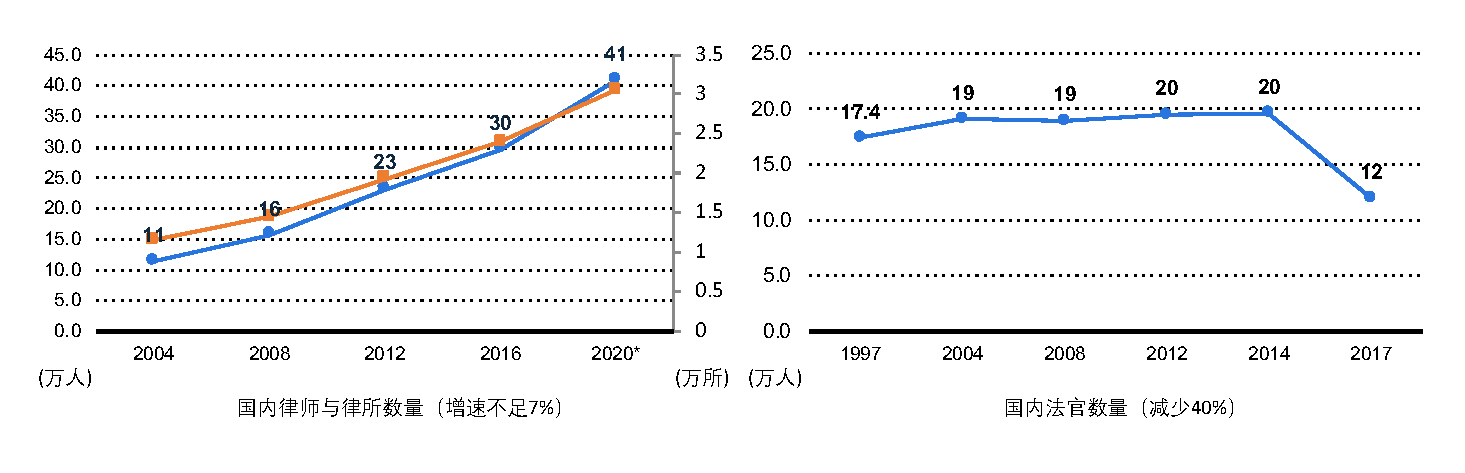
\includegraphics[width=\linewidth]{figures/professional_num}
    \caption{中国法学专业人士数量}
    \label{fig:professional_num}
\end{figure*}

\begin{figure*}[ht]
    \centering
    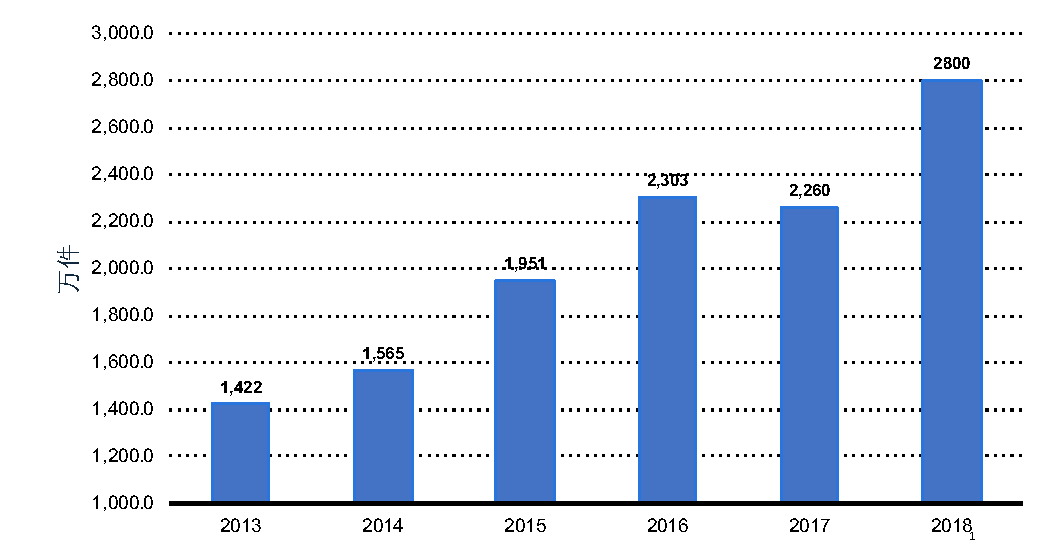
\includegraphics[width=\linewidth]{figures/case_num}
    \caption{中国法院受理案件数量(增速达\textbf{$14.5\%$})}
    \label{fig:case_num}
\end{figure*}

\textbf{法律服务需求缺口巨大。}目前,我国发生的案件中有80\%无法得到专业律师代理。与此相反,在美国人均律师数量是中国的15.6倍。同时我国律师地区分布也具有极大的差异性,80\%的律师集中在中国20\%的城市,这也就表明偏远地区人民在获取法律服务时更是难上加难。这些数据表明,法律服务在中国具有庞大的市场规模,但是由于人才供应不足,大多数人在遇到法律问题时,有求而无应。

在面临严峻考验时,最高法与众多法学专家纷纷提出相应的解决方案。其中呼声最高的便属人工智能介入司法。目前,随着深度学习的不断发展,人工智能已经上升为国家战略,其技术已经渗透到我们生活中的方方面面,而目前大量法律文本的累积以及技术的不断成熟也让人工智能介入司法成为可能。

\textbf{大量司法数据的累积。}自从国家立法以来,全国上下各级法院产生了大量的司法文件。得益于司法公开化进程推进,国家已经公开了超过6千万的法律案件文书、数千部法律与司法解释,同时,在众多的法学学者努力下创办了几百种权威的法学期刊。这为人工智能介入司法领域提供了数据基础。

\textbf{技术的高速发展。}目前,技术的创新给我们的生活带来了许许多多的改变,其中表现最突出的便是人工智能与大数据的技术。伴随着深度学习的发展,人工智能中的许多领域在近几年来取得了很大的进步。自然语言处理技术便是其中的代表,在该领域中文本分类、知识图谱、信息抽取、机器翻译等任务上,现有模型纷纷打破了前人的纪录。技术的创新带来的是生活的改变,而这样的改变也逐渐渗透到法学领域。2018年,司法部提出“加快‘数字法治、智慧司法’建设”的口号 ,这也让法学学者也越发注重人工智能在司法领域的应用。


\section{商业背景}
随着司法公开化进程的不断推进,目前市面上涌现了许多与法律服务有关的工具、平台。现有平台大多作为一个数据库检索工具,为法律工作者提供了较多的底层基础服务。经过许多年各大数据库之间的竞争与互相学习,各大数据库之间的数据与检索手段大同小异。我们将介绍目前主流平台提供的主要的法律服务:
\begin{enumerate}[1)]
	\item 案件文书、法律法规关键词检索。近几年不断涌现的法律服务平台均将案件文书、法律法规检索作为平台功能的核心。这些平台大多利用传统统计算法,获取输入关键词,计算词语匹配信息来推荐相关的文书与法条。基于关键词的检索,常常因为需要大量的背景知识来对事实进行凝练而无法普及。并且,词语匹配的检索也将受到高频无关词语的影响,而无法进行长文本检索。
	\item 法律咨询问答。许多平台意识到基于关键词的案件检索对于普通民众具有较高的知识门槛。因此为了拓宽平台受众面,许多平台纷纷与律师事务所合作,提供了法律咨询问答的服务。这些问题与“百度知道”等网络社区类似,提问者提出问题后,为回答问题者提供回馈,以吸引专业人士回答。但是这样的咨询社区因为律师数量有限、反馈不及时,同样无法提供很好的解决法律问题。
	\item 法律知识获取。为了帮助法学工作者更好获取相关知识,许多平台提供了法学期刊论文检索、书籍内容检索。这些内容以法律专业术语构成,可以帮助法学学者更好地阅读相关工作,但对于大多数人而言,该模块并无法很好帮助他们解决法律问题。
\end{enumerate}
~\\

上述功能在一定程度上能够帮助法学工作者提供相应的专业帮助,却因为功能单一、效率低而无法得到普及。即,平台提供的功能依旧无法很好帮助生活中每一个人解决法律问题。我们总结了如下现有平台面临的缺陷:
\begin{enumerate}[1)]
	\item 使用门槛高,受众范围小。基于关键词的检索,需要用户从事实中精简、总结出相关的法律专业术语,并从搜索引擎返回的结果中,利用背景知识进行筛选、重排序出对现有事实有意义的法律文书。这些操作需要很多的背景知识,这也就意味着现有平台无法面向普通人提供法律服务,这也是目前即使市面上涌现了这么多法律产品却无法为普通人提供及时、专业的法律援助的重要原因。
	\item 无法支持语义检索。目前市面上的法律服务平台采用的是传统的统计模型,即使可以支持精确检索与模糊检索,却依旧受到多个因素干扰。基于词语匹配的算法只能检索文本类似的案件文书。然而案件事实描述是一个具有很大多样性的文本,无法捕捉语义意味着检索结果具有很大的偏差。例如,检索词语“打架”,从语义角度理解,应该检索具有打架事件的事实(包括打斗、争执等词语),但是传统平台只会检索包含“打架”一词的文本。这很大程度上,限制了检索的效果。
	\item 功能单一,无法分析长文本案件。长文本检索一直以来,受到无关词语干扰重排序结果的影响,而无法很好的推广。然而对于普通人而言,长文本案情分析是非常重要的功能之一,可以降低平台使用门槛,同时尽可能多捕捉案件信息,帮助大家解决法律问题。
\end{enumerate}
~\\
因此,为了解决以上问题,团队提出了一个面向普通人的案情分析平台JudgeAI,平台从多个角度对案件进行预测分析,实现了零门槛。表格\ref{background:compare}对比了JudgeAI平台与市面上常用的法律服务产品的功能,可以发现JudageAI具有最全的功能,最低的使用门槛。

% 根据团队调研结果,市场上的产品可以大致分成两类:以搜索引擎为主体的法律文书检索系统、以检索的技术为主的问答系统。接下来我们将分别介绍这样两类系统及其代表,并简要阐述其缺点。

%文书检索系统是市面上出现最早的、目前应用也最广泛的法律应用。自从国家启动司法案例公开化之后,裁判文书网 便成为了拥有文书数量最多的官方平台,但是由于其检索速度慢、检索结果不全而没有成为一个使用广泛的工具。随后,许多其他检索工具(如无讼 、北大法宝 等)应运而生,相对于裁判文书网,这些网站增加了法律法条、指导案例的检索功能,但由于其采用的仍是基于词语匹配的检索算法,这些检索工具依旧无法从语义角度进行内容的检索,这样一个缺点在进行长文本检索时尤其突出。我们以北大法宝检索为例,在检索转化型抢劫的一般情形——“偷窃被发现,用暴力导致被害人受伤”时,北大法宝并未返回相关结果。因此,目前市场上的搜索引擎以词语匹配为技术手段,无法很好的服务于大众。

%另一类市场上较多的法律产品是以检索技术为主的问答系统。问答是自然语言处理中的热门问题,但因为效果原因并未有很好的应用,而现有产品将问题进一步简化。例如京东推出的一款名为“法咚咚”的问答产品,通过将问题限定领域,并利用现有的检索技术,在用户输入问题时,通过词语匹配技术来推荐相关的法律依据。技术的限制也让这样一个产品有了许多限制:无法分析实际情景、使用者需要有法律背景。同期搜狗提出的“搜狗律师”也面临着同样的问题。% 随着法律智能受到社会的广泛关注,各大有关公司也都推出了相应的产品。其中最具代表性的法律工具网站有:中国裁判文书网、北大法宝、法信网、法咚咚、搜狗法律等。这些产品大多以基于词匹配的案件文书检索为核心。受限于统计方法的检索能力,这些产品大多面向法律专业人士,旨在为他们提供基础的法律服务。

\begin{table}[ht]
\begin{tabular}{c|ccccc}
\hline
评价指标             & 语义检索       & 关键词标签      & 法学要素       & 案情分析预测     & 长文本检索      \\ \hline
裁判文书网            & ×          & ×          & ×          & ×          & ×          \\
北大法宝             & ×          & √          & ×          & ×          & ×          \\
威科先行             & ×          & ×          & ×          & ×          & ×          \\
无讼               & ×          & √          & ×          & ×          & ×          \\ \hline
\textbf{JudgeAI} & \textbf{√} & \textbf{√} & \textbf{√} & \textbf{√} & \textbf{√} \\
\hline
\end{tabular}
\caption{JudgeAI与市面上常用产品对比}
\label{background:compare}
\end{table}

\section{项目难点}
人工智能技术经过几十年的不断发展,已经取得了很大的进步与突破。近今年,深度学习技术受到越来越多学者的追捧,深度神经网络模型凭借着强大的自动抽取特征的能力在许多任务上超越了人类表现。同时,伴随着近几十年海量数据的不断累积、硬件高速发展带来的强大算力,神经网络已经渗透到我们生活的各个领域,并利用它强大的特征自动抽取能力,在效果上超过了传统机器学习算法,从而受到商业界、学术界的认同。但是,随着学者研究的不断深入,深度学习也逐渐暴露出其难以避免的缺点,这也给深度学习进入智慧司法领域带来了许多的困难。

\begin{figure*}[ht]
	\centering
    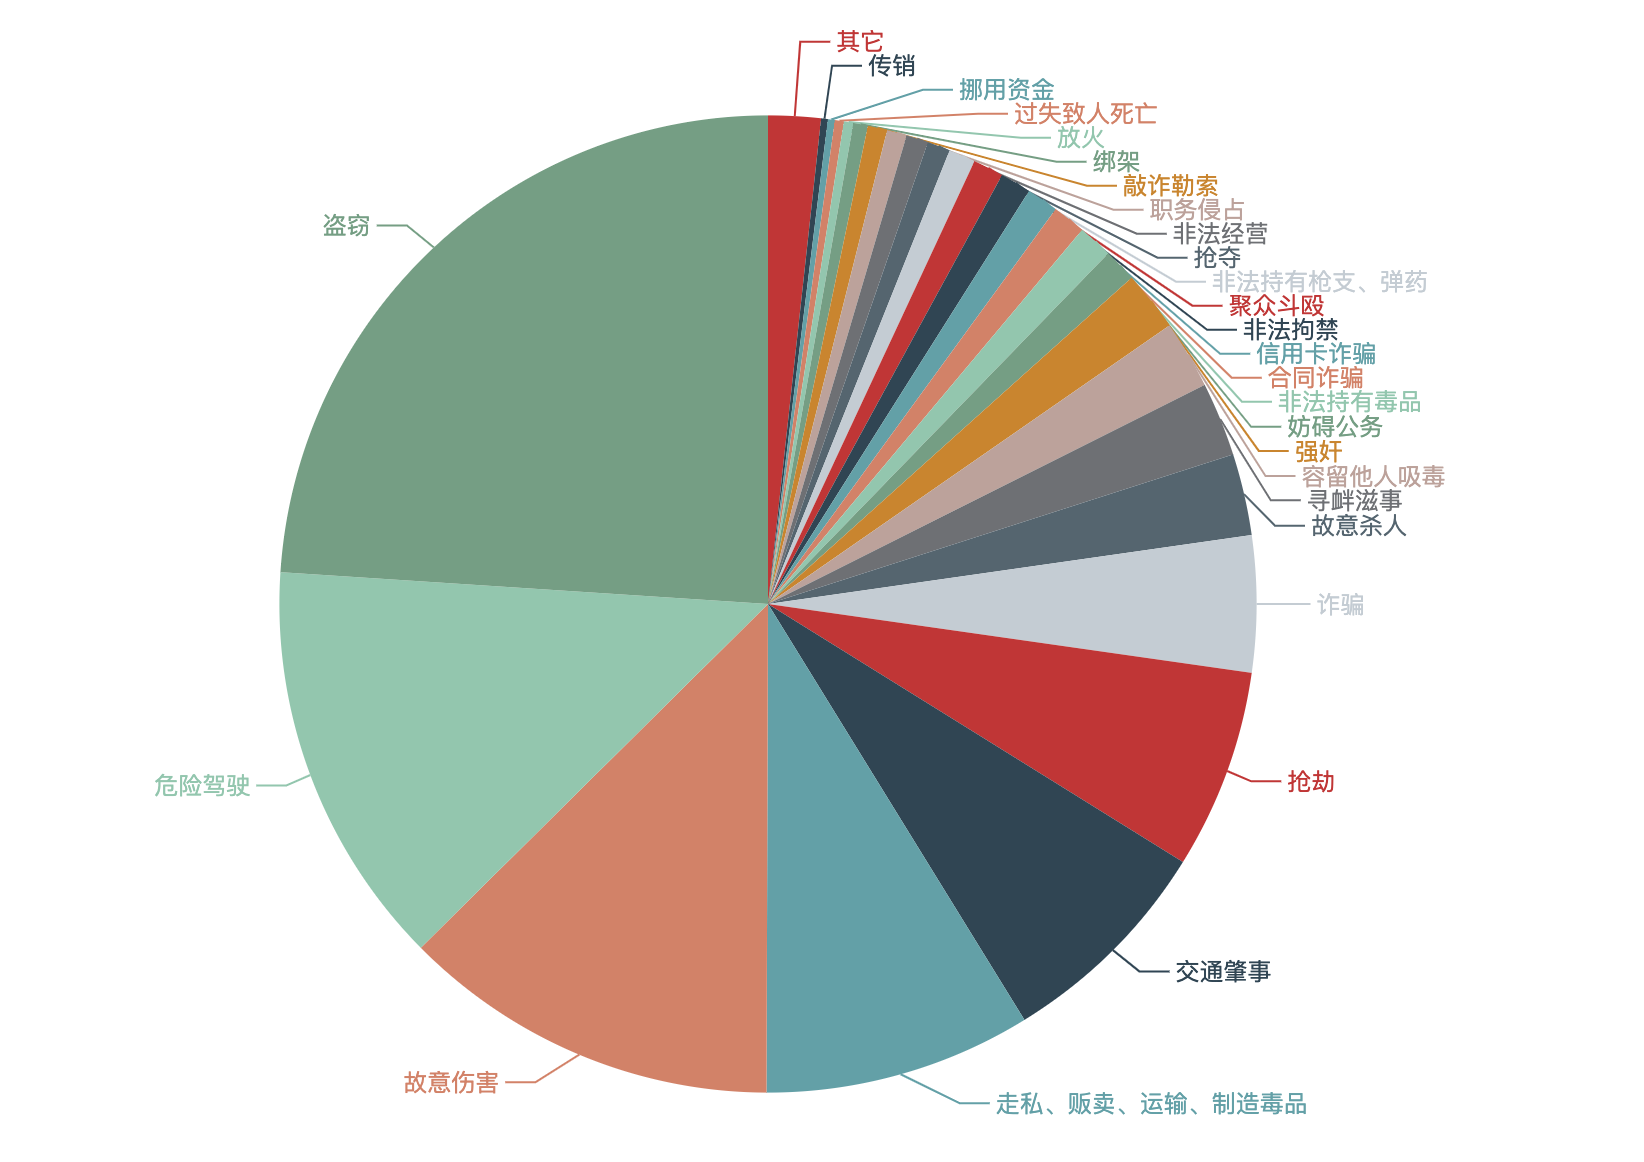
\includegraphics[width=\linewidth]{figures/case_statistic.png}
    \caption{各案件数据占比统计}
    \label{fig:case_statistic}
\end{figure*}
	
\begin{itemize}
	\item \textbf{模型不可解释性}。在深度学习系统中,分类器和特征模块都是自动学习的,这样神经网络就有了一个灰色区域:可解释性问题。而深度学习系统这样一个“黑箱”性质一直被学者们诟病。缺乏数学公式推导,给定输入,我们无法获知模型将如何产出结果,无法获知模型为何会产生这种结果。尤其是在多任务学习的深度学习系统中,系统常常产生互相矛盾的预测结果。然而在法律智能领域,模型可解释性将是极其重要的一点,任何司法问题都需要有严格的法条文本支撑、需要有严密的推理逻辑支撑。这也是自然语言处理技术发展迅速却无法在法律智能实用系统中起作用的重要原因之一。
	
	\item \textbf{知识理解差、推理能力差}。如何让深度学习系统理解知识并运用到相应的任务中一直是许多学者的目标。近几年,为了发掘深度学习系统在理解文本语义上的能力,许多学者提出了不同的阅读理解数据集\cite{nguyen2016ms,rajpurkar2016squad,trischler2016newsqa},希望能够检验模型在文本阅读、理解上的能力。通过许多年的努力,许多深度学习模型在这些数据集上的表现已经超过人类。但是模型其实并未理解文本语义,而只是有较强的文本对比匹配能力\cite{clark2018think}。\citet{kwiatkowski2019natural}实验表明,神经网络系统在需要推理的文本理解问题上表现不佳。在法律领域,如何理解海量的法律知识,并将其运用至实际生活中,是法律智能领域落地重要技术难题。
	
	\item \textbf{少样本学习}。深度学习模型早在上个世纪便被提出,然而却并没有收到学者关注,直到2012年,\citet{krizhevsky2012imagenet}将深度学习模型运用到ImageNet图片分类中,随之深度学习模型引起了人工智能领域学者的广泛关注。而之所以深度学习模型直到30年后才被发现其价值,最主要原因便是深度学习需要大规模数据训练,而上个世纪互联网没有普及,数据收集极其困难。直到现在,深度学习依旧因为“数据饥饿”的性质而受到许多的限制,少样本学习也成为许多学者关注的重点。在智慧司法领域,即使拥有数千万的法律文书,我们依旧面对着严重的数据不均衡导致的样本缺少的问题。据数据统计,刑事案件中高频的十类案件占总案件数量78.1\%,而低频的50个罪名,只占总案件数量的不足0.5\%。这也成为了法律智能系统不得不解决的重要问题。
	

\end{itemize}


~\\
%通过长时间努力,团队针对以上难点,提出了相应的解决方案,一定程度上克服并解决了上述难点给智慧司法技术落地带来的苦难。
\\

在这样的契机之下,团队构建了一个案情分析平台——JudgeAI,尝试将自然语言技术运用到法学领域的各个问题之上,旨在利用自然语言处理的技术的方法来解决实际法律问题,为大家的工作、生活提供便利。通过长时间努力,团队针对以上难点,提出了相应的解决方案,克服并解决了上述难点给智慧司法技术落地带来的困难。提出了一个创新的多任务学习框架、一套新的文本检索算法,实现了对案情的全方面多角度的分析。综合概括,JudgeAI实现了以下功能:在输入一段文本形式案情描述之后,我们平台将提供:案件的案由/罪名预测、判案要素预测、相关法条预测、相似案件检索、关键词提取和相关问题推荐的功能。以此让用户能够尽快捕捉到文本中的有用信息,并作出相应的判断,从而达到辅助判决的作用。相比于已有的产品、算法,我们团队在这些任务上提升了对长文本语义的理解,超过以往模型,达到了更高的预测精度。

\chapter{相关工作}
\label{cha:related}
当前人工智能与深度学习正在以势不可挡的冲击力影响着我们的生活,我们国家至关重要的司法领域并没有选择回避,而是采取了一个积极的姿态主动拥抱技术,其目的就是通过人工智能与法官审判制度的融合来促进司法改革。法律结合人工智能同样已经是大势所趋,法律智能这一领域也受到了学术界广泛关注,与法律智能有关的任务也层出不穷。但是,由于技术发展时间短,许多任务并未达到令人满意的效果。这也导致了目前法律智能产品虽多,却大都无法满足实际使用的需求。


% \section{学术研究现状}
\section{法律智能}

法律智能领域的研究已经持续开展了几十年,不同的学者从不同的角度提出了很多不同的法律智能任务。其中研究最为广泛的便是判决预测任务,在该任务中,算法模型需要通过阅读相关案情描述来给出判决结果,其中判决结果包括罪名、刑期、罚款等。

早在上个世纪就有许多学者尝试利用概率统计的数学模型来给出案件判决结果与事实描述词语之间的概率分布\cite{kort1957predicting,ulmer1963quantitative,segal1984predicting}。随着机器学习算法与文本挖掘算法在本世纪初的迅速发展,更多学者将判决预测抽象成一个文本分类任务,并通过手动抽取文本的浅层次特征来抽取文本信息\cite{liu2006exploring,lin2012exploiting,aletras2016predicting},并运用传统机器学习模型(朴素贝叶斯分类算法、决策树分类、支持向量机算法)来进行预测。但是这种传统做法需要耗费大量的精力总结文本规律,抽取浅层特征,并通过手动设计的规则进行预测,无法适应灵活多变的语言表示,因此并没有得到很好的运用。

到了近几年,深度学习技术高速发展,许多自然语言处理领域(NLP)中的问题都得到了很好的解决\cite{kim2014convolutional,khan2010review,tang2015document}。于是,许多学者又开始运用神经网络来结合法律知识来进行罪名的预测。例如,\citet{luo2017learning}运用NLP中常有的注意力机制,在预测过程中引入法条内容,提升预测效果;\citet{shen2018legal}利用记忆网络(Memory Network)来端到端训练相关法条预测与罪名预测任务。这些模型在相应的筛选后的测试集上取得了较好的效果,但是由于这些任务都对实际运用场景做了简化,并未考虑法官判决时碰到的实际问题,因此这些模型在实际应用中仍然无法满足需求。

总而言之,经过长时间学者们的不断努力,判决预测任务取得了较大的突破,但是几乎所有模型都对问题做出了相应的简化,导致目前判决预测任务依旧面临着很大的问题而无法落地使用。

% 法律智能领域的研究已经持续开展了几十年,早在上个世纪就有许多学者尝试用概率统计算法来对案件进行分析[1][2],通过数学模型来预测案件的判决结果。作为法律智能的基础任务,判决预测这一任务自此也受到了广泛关注,随着本世纪初机器学习算法的发展,学者们将这一任务归结为文本分类任务,并尝试通过人工抽取特征并利用传统机器学习算法(朴素贝叶斯分类、SVM算法)[3][4]预测判决结果,到了近两年,学者又将深度学习技术运用其中[5]。这些模型虽然在测试集中取得了较好的效果,但是因为对问题的简化以及未考虑到判案时的实际因素,均无法应用到实际生活中。

% 与此同时,法律智能上还有许多其他问题也受到学者们的广泛关注。例如


与此同时,受到计算机学者、法学学者共同关注的法律智能领域许多其他任务也被纷纷提出。希望能够帮助解决我们生活中的种种法学问题。例如给定案情描述判断相关法条,与判决结果预测类似,学者也尝试使用文本分类建模,利用神经网络强大的抽取特征能力,寻找最相关的法条。不仅如此,人们还尝试利用人为定义的规则构建一套系统来判断法律问题的正误,但是此类方法缺乏可拓展性,且需要耗费大量的人力物力。


总而言之,目前法律智能领域受到广大自然语言处理领域的学者的欢迎,然而因为计算机学者法律知识的相对缺乏,以及学术研究上对问题的简化,目前学术领域研究虽然取得了很大的进展,但是离技术的落地与实际应用仍有一段很长的距离。

% 通过长期的调研与讨论,我们团队提出了一个新的模型,利用了机器学习中的多任务学习机制,通过多个子任务的联合训练提升了各个任务的效果;同时,考虑到法官的判案经过,我们提出了一个完整的模拟法官真实判案过程的模型,超过了之前提出的baseline模型,达到了真实可用的效果。





% \section{类案检索}

% \section{商业产品现状}

% 综上所述,目前市面上的法律产品并没有使用人工智能领域的前沿技术,而其服务的受众群体也是极其有限的,无法律知识背景的人在使用这些工具时会遇到很大的困难。


\chapter{项目创新点与意义}
\label{cha: significance}

\section{项目创新点}

在学术研究上,团队尝试应用自然语言处理技术解决实际生活中的法学问题。通过长时间的探索与交流,我们总结并提出了多个常见的法学任务,并将其形式化为能够利用自然语言处理模型进行处理的常见任务。并且在多个任务上,团队提出了创新性的模型,达到了不错的效果。

另一方面,通过与法律从业人员长时间的沟通交流,团队提出的任务都是建立在切实解决实际问题的基础之上的。我们致力于打造一个功能全面、技术可靠的案情分析平台。相比于市面上现有的一些法律产品,我们平台的功能更加全面、实用,结果更加可靠。

总结而言,项目有以下亮点与创新:
\begin{enumerate}[1)]
	\item 尝试利用自然语言处理的最前沿的技术解决相关的法律问题。通过对案由预测、相关法条预测、刑期预测、关键词抽取、类案推荐等功能的实现,平台可以帮助法律领域从业人员减免重复工作,成为辅助其工作的好工具;同时也可以为大家身边遇到的法律问题提供的解决方案,成为无法学背景的非专业人士的好帮手。
	\item 提出了全面的法学基础任务,能够对每一段案情进行多角度全方位的分析,更好的满足了用户需求。通过与从业人员的多次的深入交流,我们获知了他们在工作中碰到最多的几大问题,并进行针对性的解决,真正做到了充分了解用户需求。
	\item 在判决预测模块,我们提出了一个能够捕捉子任务间依赖关系的多任务学习模型,超过了以往模型,实现了state-of-the-art效果。在我们提出的几个任务之间,往往有着很强的依赖关系,例如案由与法条之间具有很强的映射关系。模型通过捕捉这些子任务之间的映射关系,提升其效果。
	\item 首次在关键词抽取任务上运用并改进Lattice-LSTM模型。克服了词级别模型过度依赖于中文分词效果、字级别模型语义信息不足的缺点,在传统的序列标注模型上实现了大幅提升。
	\item 在类案检索模块,我们提出了一个基于关键词抽取、案件语义理解的模型,做到了在语义层面上的相似性检索。模型首先抽取案情关键词标签,通过标签缩小候选的相似文本集合,再进一步通过不同文章的文章向量之间的距离来衡量案情的相似程度。相比于传统搜索引擎的文本相似性检索,此搜索模块可以做到真正的语义相似性检索。
\end{enumerate}

\section{项目意义}
人工智能现已上升为国家战略,各行业各领域也纷纷响应并加入到这场人工智能的改革当中。法院作为保障社会公平公正的重要一环,与社会生活密切相关。把大数据、人工智能与司法体制改革结合起来,将会给司法工作注入前所未有的创造力。

现在全国3519个法院和9279个人民法庭通过专网已经实现了互联互通,各级法院以每分钟一次的频率向最高人民法院大数据管理和服务平台自动汇集新收集的各类案件数据,目前该平台已汇集了1亿多件案件数据和$6,000$万份法律文书。显然,人工智能介入司法领域是时代发展的必然趋势。当前案多人少的严峻局面并没有因司法改革的深入得到根本性转变。以2015年和2016年为例,全国各级法院审结一审刑事案件分别为$109.9$万件和$111.6$万件,分别比上年增加了$7.5\%$和$1.5\%$,有许多基层法院刑事法官年均结案数量已达200件以上。在员额法官增加受体制钳制的情形下,通过人工智能来提高审判工作效率是一个必然选择。

况且分析近十年依法纠正的三十余件重大冤假错案发生的原因,可发现既有事实不清,更有证据收集上的不规范、数量上的不充分、标准上的不一致,严重背离了“证据三性要求”和排除合理怀疑的定罪标准,当然也不排除其中人为意志因素的干扰。这就需要利用司法大数据对这些问题案件进行全面梳理以分析原因、发现问题、总结经验、制定标准和规则,并将证据收集要素嵌入人工智能模块,进而为司法人员合法有效收集证据提供确切指引,以避免以往的随意性或不规范性。显然,人工智能所体现出的智能性和高效性与司法人员的创造力结合起来构建人力和科技深度融合的司法运行新模式,这是以审判为中心诉讼制度改革的应有之义。

总而言之,项目的完成有着以下的意义:
\begin{itemize}
	\item 在专业人员数量受限制的情况下,平台可以在保障审判质量的同时,利用人工智能算法来大大提升审判工作的效率。
	\item 排除人为意志因素对审判结果的干扰,利用司法大数据对判案制定统一的标准。
	\item 成为每一个人的法律咨询助手,平台提供了详细、全面的案件案情分析,能够很好地为每一个人提供法律知识,帮助大家维护自身权益。
	\item 提供了人工智能与司法人员结合的判案新模式,这将是未来的发展新模式。
\end{itemize}





\chapter{平台功能与成果概述}

\section{功能介绍}
平台围绕着输入的案情描述进行了全方面多角度的分析,我们实现以下几个功能:

1)	罪名/案由预测,输入一段案情后,模型通过获取其语义,给出相关的案由/罪名及相关概率;

2)	相关法条推荐,对案情进行分析后,模型将给出与案件有关的法律法规;

3)	刑期预测,对每一个刑事案件,模型都将给出可能的判罚刑期,我们将刑期合理的划分成几个区间,模型将给出被告判罚的刑期落入每一个区间的概率;

4)	关键词抽取,通过序列标注模型,模型为每一个输入案情给出相应的法学关键词;

5)	类案推荐,在输入案情描述之后,我们将在数据库中进行检索,并通过模型计算,给出在语义层面与输入案件相关的法律文书。


\section{成果概述}

通过长时间的努力,团队取得了许多阶段性成就。

1)	大规模的法律文书数据集,通过长时间分布式的数据抓取,我们最终获得了数千万的法律文书,其中包括刑法500余万份;

2)	关键词抽取数据集,为了实现关键词抽取模型,我们整理了10000万份待标注的法律相关句子,通过专业人士的人工标注,我们最终获得了这样一份高质量的关键词抽取数据集;

3)	判决预测模块算法的实现,提出了一个新的多任务学习模型,取得了很好的效果;

4)	关键词模块算法的实现,将目前自然语言处理领域最前沿的序列标注模型应用至关键词抽取任务上,通过特征工程等方法,对算法进行了改进;

5)	类案推荐搜索引擎的实现,提出两步走的检索算法,做到了语义相似性检索;

6)	平台搭建,将所有算法集成到demo平台上,形成一个可用的法律产品。

\chapter{算法实现}
本章,我们将从判决预测、关键词抽取、类案搜索等模块来详细介绍项目中用到的算法模型。在模型中,我们统一使用了THULAC进行中文分词,我们使用的词向量是利用FastText模型,在大规模的法律文书语料库上进行的预训练,我们采用的词向量维度为200维。

对于每一个模块,我们将分别从任务的描述定义、算法的创新点、算法模型细节三个方面来进行详细阐述。


\section{背景知识}
\iffalse
\subsection{卷积神经网络}

卷积神经网络(Convlutional Neural Network, CNN)是多层感知机(Multi-Layer Perceptrons, MLP)的变种,由生物学家在早期关于猫视觉皮层细胞的深入研究发展而来,猫视觉皮层的细胞存在一个非常复杂的构造,这些细胞对视觉输入空间的某些子区域非常敏感,称之为感受野。

CNN的本质是一个多层感知机,成功的原因在于它所采用的局部连接和权值共享的方式:1)一方面减少了权值的数量,这样使得神经网络更加容易被优化;2)另一方面它降低了模型的复杂度,即减小了模型过拟合的风险。

这些优点在模型的输入是图片时表现得更加明显,它使得图像可以直接作为网络的输入,避免了传统识别算法中复杂的、耗费大量人力的特征提取和数据重建的过程,因此在CNN在图像的处理过程中具有非常大的优势,因为网络能够自行抽取图像的特征包括颜色、纹理、形状及图像的拓扑结构,在处理二维图像的问题上,特别是识别位移、缩放及其他形式扭曲不变性的应用上具有很强的的鲁棒性和运算效率等

\subsection{网络结构}
卷积神经网络是一种带有卷积结构的深度神经网络,卷积结构可以减少深层网络占用的内存量,其三个关键的操作,其一是局部感受野,其二是权值共享,其三是池化层(Pooling layer),减少了网络的参数数量,缓解了模型的过拟合问题。

卷积神经网络是一种多层的监督学习神经网络,隐含层的卷积层和池采样层是实现卷积神经网络特征提取功能的核心模块。该网络模型通过采用梯度下降法最小化损失函数对网络中的权重参数逐层反向调节,通过频繁的迭代训练提高网络的精度。卷积神经网络的低隐层是由卷积层和最大池采样层交替组成,高层是全连接层对应传统多层感知器的隐含层和逻辑回归分类器。第一个全连接层的输入是由卷积层和子采样层进行特征提取得到的特征图像。最后一层输出层是一个分类器,可以采用逻辑回归,Softmax回归甚至是支持向量机对输入图像进行分类。


\begin{itemize}
	\item \textbf{卷积层(Convolutional layer)}:卷积神经网路中每层卷积层由若干卷积单元组成,每个卷积单元的参数都是经过\textbf{反向传播算法}训练得到的。卷积运算的目的是提取输入的不同特征。
	\item \textbf{线性整流层(Rectified Linear Units layer, ReLU layer)}:使用线性整流作为激活函数。它可以增强判定函数和整个神经网络的非线性特性,而本身并不会改变卷积层。
	\item \textbf{池化层(Pooling layer)}:通常在卷积层之后会得到维度很大的特征,将特征切成几个区域,取其最大值或平均值,得到新的、维度较小的特征。
	\item \textbf{全连接层(Fully-Connected layer)}:完成从输入到标签集的映射,即分类。
\end{itemize}

\begin{figure*}[h]
    \centering
    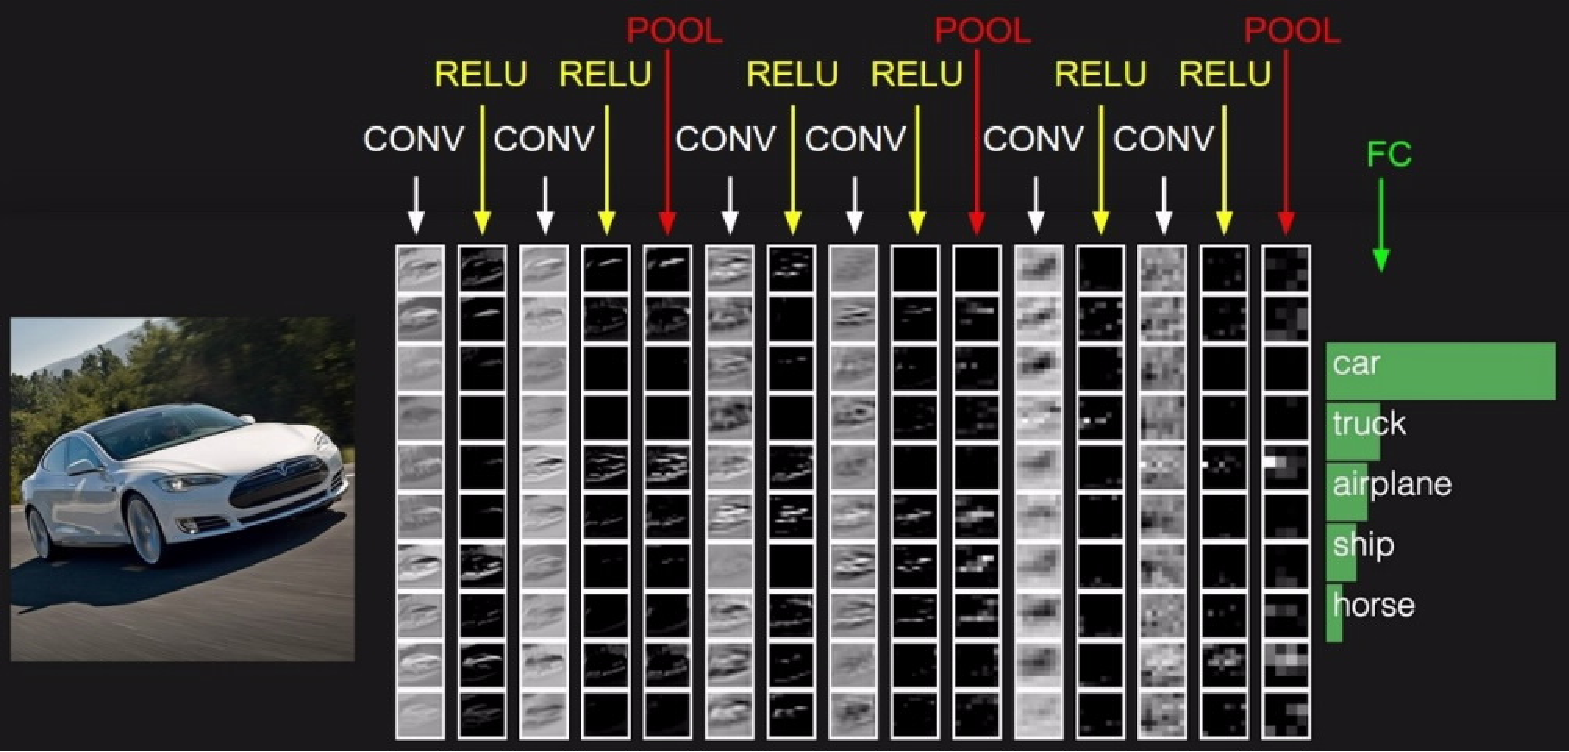
\includegraphics[width=\linewidth]{figures/cnn1}
    \caption{卷积神经网络实例}
    \label{fig:cnn1}
\end{figure*}

图~\ref{fig:cnn1}是一个卷积神经网络各层应用的实例:


卷积神经网络中最基础的操作是卷积。基础 CNN 所用的卷积是一种 2-D 卷积。也就是说,卷积核(kernal)只能在 x,y 上滑动位移,不能进行深度(跨通道)位移。

卷积需要输入两个参数,实质是二维空间滤波,滤波的性质与卷积核选择有关,CNN 的卷积是在一个 2-D 卷积核与 2-D 输入映射之间,在各通道分别完成的。

我们假设单一通道输入的空间坐标为 ${\displaystyle (x,y)}$,kernel 大小是 ${\displaystyle p \times q}$,kernel 权重为 ${\displaystyle w}$,图像亮度值是 ${\displaystyle v}$,卷积过程就是 kernel 所有权重与其在输入图像上对应元素亮度之和,可以表示为:${\displaystyle conv_{x,y} = \sum_i^{p*q}w_i v_i}$。

下面即是一个例子:

\begin{figure*}[ht]
    \centering
    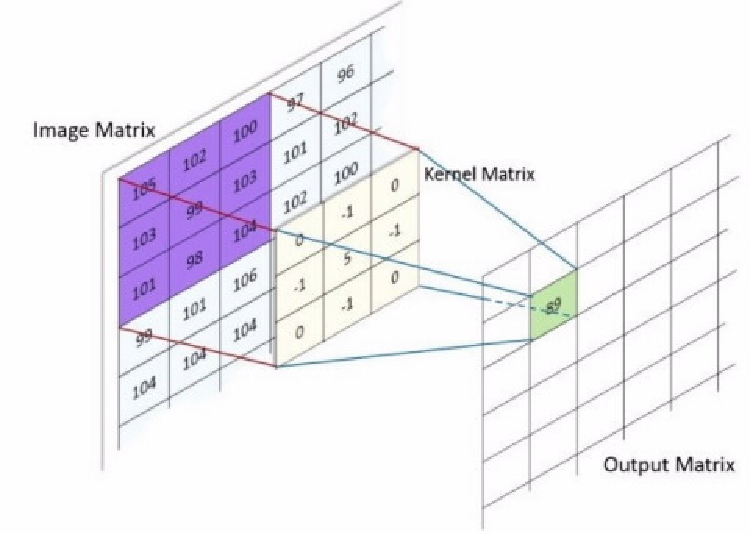
\includegraphics[width=\linewidth]{figures/cnn_conv}
    \caption{卷积层的例子}
    \label{fig:cnn_conv}
\end{figure*}

将 kernel 随 ${\displaystyle (x,y)}$ 平移扫描,即可以得到输出空间。需要特别说明的是,卷积层可能包含多个 kernel,用以抓取多个特征;扫描步长、方向也可能有所不同。

卷积之后,通常会加入偏置(bias),并引入非线性激活函数(activation function),令偏置为 ${\displaystyle b}$,激活函数为 ${\displaystyle h\left(\right)}$,经过激活函数后,得到的结果是 ${\displaystyle z_{x,y}=h\left(\sum_i^{p*q} w_i v_i +b\right)}$。

池化(Pooling)是卷积神经网络中另一个重要的概念,它实际上是一种形式的降采样。有多种不同形式的非线性池化函数,而其中“最大池化(Max pooling)”是最为常见的。它是将输入的图像划分为若干个矩形区域,对每个子区域输出最大值。直觉上,这种机制能够有效地原因在于,在发现一个特征之后,它的精确位置远不及它和其他特征的相对位置的关系重要。池化层会不断地减小数据的空间大小,因此参数的数量和计算量也会下降,这在一定程度上也控制了过拟合。通常来说,CNN 的卷积层之间都会周期性地插入池化层。

池化层通常会分别作用于每个输入的特征并减小其大小。目前最常用形式的池化层是每隔 2 个元素从图像划分出 ${\displaystyle 2\times 2}$ 的区块,然后对每个区块中的 4 个数取最大值。这将会减少 75\% 的数据量。

出现在 CNN 最后的全连接层的主要目的是分类。这与神经网络中的全连接层是相同的。

CNN 网络的训练一般使用反向传播(Back Propagation)算法。同样地,这即是传统神经网络训练的常用算法。


\subsection{长短时记忆网络}

长短时记忆网络(Long short-term memory, LSTM)是一种用于深度学习领域的循环神经网络(Recurrent Neural Network, RNN)架构。与其他神经网络架构不同,LSTM 网络非常适合基于时间序列数据进行分类、处理和预测。

循环神经网络相比全连接神经网络更擅长处理序列数据,与传统神经网络不同,它们是具有循环的网络,这将允许信息持续存在。

咕咕咕,这里有一张图

上图是一个示意图,一组神经网络 A 接收某些输入 ${\displaystyle x_t}$,并输出一个值 ${\displaystyle h_t}$。循环允许信息从网络的一个步骤传递到下一个。

RNN 的重要能力在于它可以将以前的信息连接到当前任务,例如使用先前的视频帧来帮助对当前帧的理解。然而,对于较长距离的历史信息,RNN 仍无法有效地将其利用。

LSTM 相对 RNN 而言解决了长依赖关系学习的问题,能够记住长时间间隔内的信息。通常地,一个 LSTM 单元包含细胞、输入门、输出门和忘记门。其中,细胞(用${\displaystyle C_t}$ 表示)用于记录需要的长时间间隔的信息;输入门、输出门、忘记门具有删除或添加信息到细胞状态的能力,它们被用于维护细胞的状态、控制进出单元的信息流。

下图是一个示意图:

咕咕咕,这里有另一张图
\fi

\subsection{条件随机场}

\subsection{Word2vec算法}
Word2vec算法是Google在2013年开源的一个可以将词语映射到低纬向量空间的的算法。该算法就离散的词语转化成连续向量空间中的向量,并可以利用向量之间的关系计算出词语的相似度,同时作为一种词语的表示,word2vec也受到了非常多学者的欢迎。

Word2vec算法中有两类主要模型,分别是 $CBOW$ ($Continuous Bag-of-Words Model$) 和 $Skip-gram$ ($Continuous Skip-gram Model$) 模型。两种模型都采用神经网络计算语言模型,结构都大致可分为输入层、投影层和输出层三层结构。

在这里我们重点介绍 $CBOW$ 模型。它是在已知当前词 $x_i$ 的上下文 $\{x_{i−2}, x_{i−1}, x_{i+1}, x_{i+2}\}$ 词向量 $\{w_{i−2}, w_{i−1}, w_{i+1}, w_{i+2}\}$ 的基础上预测当前词 $x_i$ 的词 向量 $w_i$,网络结构如图

\section{判决预测}
\subsection{任务描述}
司法的一个重要作用便是对现实生活中发生的各类纠纷、案例以及违法法律的情况进行裁决,而判决就是体现这个裁决的重要场景,而判决结果是每一个案件最关键的基础特征,为了能够直观地捕获到案件的核心特征,在该模块中,\textbf{我们实现了对法学判案要素预测、案件的罪名/案由判断、相关法条推荐、量刑预测功能}。

这四个任务的结果之间具有很强的前后依赖关系,例如,最终量刑强烈依赖于法条的相关规定。在该模块中,四个任务按照顺序构成任务序列,分别对应于模型中$task_{1}$至$task_{4}$。

输入一段文本形式的案情描述,模型通过阅读文本获取其中蕴含的语义信息,将案情映射到高维向量空间,得到一个蕴含关键判案信息的文章向量。在该模块中,我们应用了多任务学习模型(multi-task learning),利用相同的编码器捕获文本信息,通过对每一个任务设置不同的输出层,将高维文本向量映射到不同的输出结果之上。
%再根据不同的任务,将文章向量喂给不同的输出层获得不同的分类结果。

\begin{figure*}[ht]
    \centering
    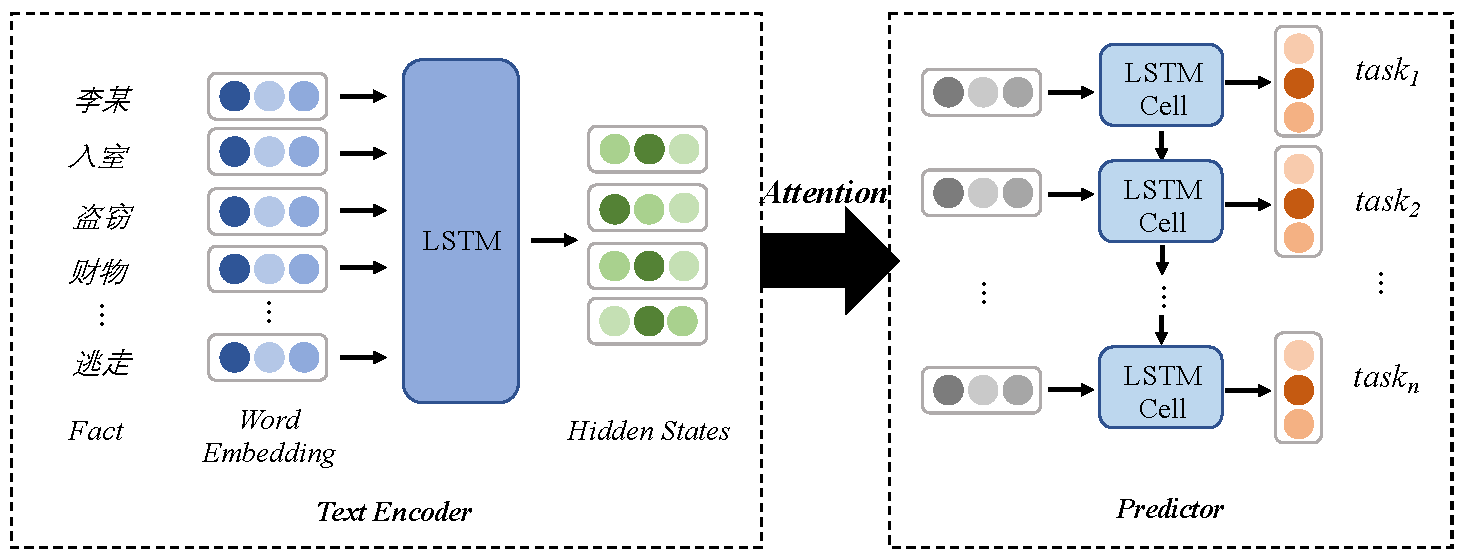
\includegraphics[width=\linewidth]{figures/model1}
    \caption{判决预测模型示意图}
    \label{fig:model1}
\end{figure*}

\subsection{创新点}
我们将上述问题总结为文本分类问题,然而由于无法考虑到在实际法律场景运用中的数据不均衡、相似罪名难以区分等问题,传统文本分类模型在这些任务上无法取得令人满意的效果。通过观察基线模型的预测效果,我们发现了以下现有模型无法解决的难点:
\begin{itemize}
	\item \textbf{数据不均衡(Few-shot)}。在实际场景数据集中,不同案由的案件数量具有极度不均衡性。根据我们对裁判文书网上刑事案件的统计,实际生活中遇到的案件,最频繁发生的十类案件数量(例,盗窃案件、故意伤害案件等)达到了总案件数量的$78.1\%$,然而与此正相反,频率最低的50个罪名案件数量(例,扰乱法庭案、逃税案)只占案件总数量的不到$0.5\%$。以往模型往往关注在高频案件,而忽略了低频案件的判决,然而低频罪名的判决恰恰需要更加大量的法律专业知识。低频罪名的判断也成为提高判决系统稳定性、实用性的关键所在。
	\item \textbf{易混淆罪名难以辨析}。在我国法律体系中存在很多相似的易混淆罪名(例如,盗窃与转化型抢劫、挪用公款罪与贪污罪)。细微的事实改变就可以改变被告罪名判决结果,以往模型在这些罪名上将出现大量的混淆。
	\item \textbf{预测结果矛盾}。传统模型在预测多个任务时,往往因为无法正确捕捉任务之间的依赖关系而预测出矛盾的结果。以往模型往往会预测出完全无关的相关法条、罪名与刑期等,例如模型预测被告为盗窃罪,在刑期上却预测出死刑。预测结果的矛盾导致了以往模型无法运用到实际。
\end{itemize}

在此基础上,我们提出了一个新的判决预测模型,该模型能够捕捉到不同任务之间前后依赖关系,同时通过模拟人类法官判案思路,将判断案件法学要素作为预测判决结果的子任务来提升模型在混淆罪名与低频罪名上的预测效果。综上,我们做出了以下贡献:
% 我们将上述所有功能归纳为文本分类问题,通过观察,上述任务之间有很强的前后依赖关系,例如,相关法条推荐结果往往与罪名及案由预测结果高度相关。并且,根据法学领域从业人员介绍,在实际判案时,大家首先会判断案情中的相关要素,并根据要素判断结果来决定最后的案件的判决。因此,我们有以下创新来提升各个任务的效果:

\begin{itemize}
	\item 提出了一个新的具有高度可扩展性的多任务学习(multi-task learning)模型,相比于以往多任务学习模型,我们的模型可以充分利用各个任务之间的依赖关系,避免了不同任务之间预测结果的矛盾性,同时提升了模型在多个任务的预测效果。
	\item 提出了判决预测新的子任务——判案要素预测,模型通过预测不同案件之间共有的法学要素,来提升模型对法律案件的特征抽取能力。在低频案件的预测上,相比于基线模型,我们的模型实现了超过50\%的效果提升。我们采用了10个最常见的判案要素,如表格\ref{tab:key_elements}所示,要素判断结果可以很好地帮助我们对案件被告涉及罪名做出判断。
	\end{itemize}

\begin{table}[]
\center
\begin{tabular}{l|l}
\hline
\textbf{要素}          & \textbf{要素描述}   \\ \hline
盈利          & 被告犯罪是否以盈利为目的       \\
买卖          & 被告行为中是否涉及买卖行为      \\
死亡          & 被害人是否死亡            \\
暴力          & 被告是否采用了暴力手段犯罪      \\
国家机关/国家工作人员 & 案件中是否涉及国家机关与国家工作人员 \\
公共场合        & 案件是否发生在公共场合        \\
非法占用        & 被告是否以非法占用为目的       \\
伤害          & 被害人是否受伤            \\
主观故意        & 被告主观上是否故意犯罪        \\
生产作业期间      & 案件是否发生在生产作业期间  \\ \hline   
\end{tabular}
\label{tab:key_elements}
\caption{判案要素表}
\end{table}


\subsection{算法模型}
% 算法使用了LSTM作为模型的编码器,使用了全连接神经网络作为输出层。利用了多任务学习的框架,将多个任务进行联合训练得到了效果的提升。
输入案情文本描述后,我们将其进行分词操作将案情描述划分为词语序列$x = \{x_{1}, x_{2}, ..., x_{n}\}$,其中$n$为词语数量。同时,模型适用于multi-task learning任务,我们假设有案件预测结果为$T$,其中$Y = \{y_{1}, y_{2}, ..., y_{|T|}\}$,$y_{i}$为第$i$个子任务的结果。

在该模型中,我们利用长短时记忆网络(LSTM)作为文本编码器,生成案情文本的表示向量。LSTM是循环神经网络的一个变种,通过在每一个循环单元引入输入门、遗忘门、输出门和记忆单元来帮助神经网络捕捉长序列的信息。考虑到我们的输入文本较长,为了捕捉长文本序列关系,我们采用了LSTM作为编码器。编码器结构可分成以下几层。
\begin{itemize}
	\item \textbf{输入层}:文本分词与词向量映射。在获取到输入文本后,我们采用了THULAC作为文本分词器对文本进行分词,同时我们采用了FastText模型在数据集上预训练了词向量。在本层,通过查词向量表,我们将每一个输入单词$x_{i}$转换成词向量$\mathbf{x}_{i}$。此时,输入的文本已经被转换成
	\begin{equation}
		\hat{x} = \{\mathbf{x}_{1}, \mathbf{x}_{2}, ..., \mathbf{x}_{n}\}
	\end{equation}
	\item \textbf{编码层}:为了能够让捕捉到词语序列前后文信息,我们用LSTM对获取到的词向量进行编码处理,获得隐向量序列$\mathbf{h} = \{\mathbf{h}_{1}, \mathbf{h}_{2}, ...,\mathbf{h}_{n}\}$。其中
		\begin{equation}
			\mathbf{h}_{i} = LstmCell(\mathbf{x}_{i}, \mathbf{h}_{i-1})
		\end{equation}
	\item \textbf{注意力层}:我们在循环神经网络基础之上运用了注意力机制(attention)捕获输入文本中的关键信息。通过attention机制,我们可以根据任务的不同,捕获到不同的关键信息,从而为每一个任务都生成一个不同的表示向量$\mathbf{a} = \{\mathbf{a}_{1}, \mathbf{a}_{2}, ..., \mathbf{a}_{n}\}$。其中,$\mathbf{u}^{k}$为每个子任务的表示向量,$\mathbf{W}^{a}$为训练参数。
		\begin{equation}
			\mathbf{a}_{i} = \sum_{j=1}^{n}\alpha_{j}\mathbf{h}_{j}
		\end{equation}
		\begin{equation}
			\alpha_{j} = \frac{exp(tanh(\mathbf{W}^{a}\mathbf{h}_{j})^{T}\mathbf{u}^{k})}{\sum_{t}exp(tanh(\mathbf{W}^{a}\mathbf{h}_{t})^{T}\mathbf{u}^{k})}
		\end{equation}
	\item \textbf{预测层}:在为每一个任务获得其表示向量后,我们利用了LSTM Cell捕捉长序列信息的能力来获取前后任务之间的依赖关系。我们将Attention层的输出当做预测层的输入序列,为每一个子任务初始化一个不同的LSTM单元,从而获取与任务相关的文本表示向量$\hat{\mathbf{ht}}_{i}$。
		\begin{equation}
			\hat{\mathbf{ht}}_{i} = LstmCell(\mathbf{a}_{i}, \mathbf{ht}_{i})
		\end{equation}
		\begin{equation}
			\mathbf{ht}_{i} = \mathbf{W}_{i}\mathbf{ht}_{i-1} + \mathbf{b}_{i}
		\end{equation}
	\item \textbf{输出层}:最后,在获得每一个任务特有的文本表示向量之后,我们采用了全连接神经网络,将包含任务信息的文本向量映射到每个任务相应的分类中。对于每个不同的任务而言,$\mathbf{y}_{i} \in \mathbf{Y}_{i}$,其中$\mathbf{Y}_{i}$是每个任务的分类空间,例如对于罪名预测任务而言,$Y =$\{盗窃罪、抢劫罪……\}
		\begin{equation}
			\mathbf{y}_{i} = softmax(\mathbf{\hat{W}}_{i}\mathbf{ht}_{i} + \mathbf{\hat{b}}_{i})
		\end{equation}
	
\end{itemize}

我们采用了交叉熵损失函数,运用了Adam算法训练模型参数。其中损失函数计算公式如下,
\begin{equation}
	\mathcal{L} = \sum_{j}\mathcal{L}_{j}
\end{equation}
\begin{equation}
	\mathcal{L}_{j}(\hat{\mathbf{y}_{j}}, \mathbf{y}_{j}) = -\sum_{k=1}^{|Y_{j}|}\mathbf{y}_{j, k}log(\hat{\mathbf{y, k}})
\end{equation}

我们将算法运用于判案要素预测、罪名预测、法条预测、刑期预测四个任务上,四个任务的预测结果前后依赖,罪名预测结果依赖于要素预测结果,刑期预测结果与法条内容高度相关。因此,我们将四个任务按照上述顺序构成任务序列,利用任务之间的相关关系,提升各个任务的效果。具体实验结果见章节\ref{cha:result}。


\section{关键词抽取}
\subsection{任务描述}
关键词抽取旨在从信息化的文本中,提取出最重要的成分,通过有限个的关键词,尽可能的还原信息化文本中原本的含义。在传统的数据挖掘中,关键词抽取的方法被用在了各种各样的数据上,提取出的关键词可被用于检索、分类等多种具有实用性的任务中,并起到核心作用。可以说,关键词抽取的技术不仅可以让我们更好的从文本中提取信息,还可以在海量的信息化文本中构建起特征的桥梁。

虽然传统的关键词抽取方法已经被广泛应用,但是它也存在着许多不可避免的问题。在传统方法中,基于词频、词性特征的关键词抽取算法,需要大量的人工介入,在许多领域并不可行,特别是在司法领域。在司法领域中,由于复杂的语言环境、司法化的特有描述、频繁出现的各式各样的人名与地名等因素,现有的所有分词方法均不能很好的处理智慧司法中信息化的文本,因此传统的基于分词的关键词提取技术在司法领域无法发挥很好的效果。

因此,我们提出了一种基于栅栏式长短时记忆神经网络(Lattice-LSTM)的关键词抽取算法。模型在字级别模型框架基础上,融合了所有可能的词语信息,在短文本关键词抽取上模型效果有着显著的提升。

任务输入为一段案情描述的文本,任务的输出为文本中包含的关键词语,这些词语作为文本的法律标签,是用来检索相关案件、法条的重要依据。例如,对于句子:“被告对{\color{red}火灾}发生是否存在{\color{red}过错},应否对原告的合理损失予以{\color{red}赔偿}”中标红的即为关键词,这些关键词可以很好地帮助检索相关法律法规:“关于{\color{red}火灾过错}引发事故责任划分与{\color{red}赔偿}…”。

本模型的训练数据为筛选过后的法律咨询问句,法律文书中的描述案件争议焦点的句子。我们总共整理了10000条待标注数据,通过人工标注的方法,构建了关键词抽取数据集。

在使用时,我们将对每一个句子进行关键词抽取,筛除其中逆文本频率低的词语,将所有句子的关键词进行合并、筛选,得到最终文章级别的关键词。关键词抽取的结果将对后续的相关案例检索提供重要的帮助。

\subsection{创新点}

关键词抽取是自然语言处理领域非常重要的一个任务,提取出的关键词可以用于文本摘要生成、信息检索、问答等下游任务上。传统的关键词抽取算法(TextRank、LDA、TFIDF)已经被应用到许多领域,但是因为其过多依赖于词频、词性等特征而受到文本处理工具效果的限制。

随着深度学习技术的发展,学者提出了许多有监督的关键词抽取算法,在传统基于词频的无监督学习算法的基础上取得了较大的突破。这些模型大体可分为字级别模型与词级别模型。词级别模型与传统无监督学习算法一样,模型依赖于前序分词的效果,导致了最终模型错误的累积。而不少工作已经证明字级别模型因为缺乏词语信息而无法准确抽取文本中关键词。

本项目所要解决的技术问题是:如何提供一种新的不依赖于分词的关键词抽取技术,能够应对智慧司法领域中可能出现的各种输入,例如人名、地名等,做到在复杂的语言环境下提取文本特征,最终提高关键词抽取在智慧司法领域的效果。

团队提出了基于Lattice-LSTM的关键词检索算法,算法在字级别模型的基础上融合了文本中所有可能的词语信息。综上所述,模型有以下创新:
\begin{itemize}
	\item 模型以字模型为基础,将词语的信息有效融入模型中,实验表明,相比于以往关键词抽取算法,模型实现了6\%的效果提升。
	\item 模型充分考虑了文本中所有可能出现的词语的信息,可以有效避免前序步骤分词效果不佳而导致的关键词抽取不准确的缺点。
\end{itemize}

%在早期,大多数人们使用的是基于词频等特征的无监督学习算法,例如TextRank、LDA、TFIDF算法。对于法律这样一个特定领域,关键词抽取的结果往往是一些法言法语,相比于开放领域上的关键词抽取,有着更强的规律性。因此,我们将目前效果最好的命名实体识别算法运用至该任务。同时,由于训练是在句子级别的语料上进行训练,我们设计了筛选算法,将在所有句子上的抽取结果进行合并筛选,得到了一个较好的效果。

\subsection{算法模型}

\begin{figure*}[ht]
    \centering
    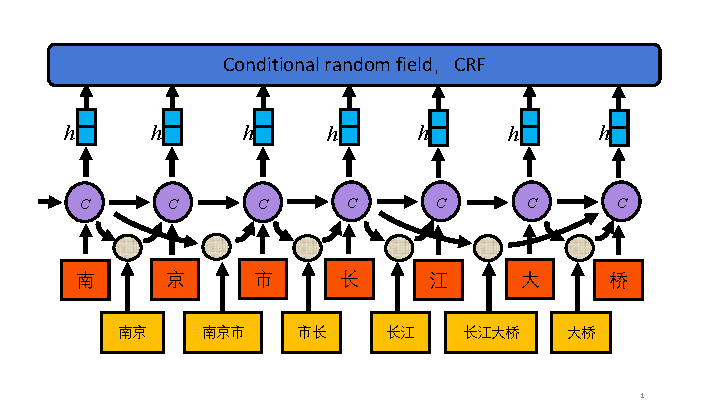
\includegraphics[width=\linewidth]{figures/key_word}
    \caption{关键词抽取模型示意图}
    \label{fig:model2}
\end{figure*}

关键词抽取模型可分为以下几个模块:

\textbf{文本编码模块}。给定待抽取关键词的一个句子实例x,其句子可以拆分为字的序列$\{x_{1}^{c},x_{2}^{c}… x_{L}^{c}\}$,同时连续的相邻几个字还有可能会组成一个词,用$x_{(b,e)}^{w}$表示一个由$\{x_{b}^{c},x_{(b+1)}^{c}… x_{e}^{c}\}$构成的词。我们将句子中包含的字与词的信息${x^{c},x^{w}}$共同作为文本编码模块的输入。具体来看,文本编码模块主要分为输入层和编码层两个层级。
\begin{itemize}
	\item \textbf{输入层}。文本编码模块的输入包含字序列与词信息两部分,输入层的功能就是将输入的字与词转化为对应的低维语义向量。对于字的语义向量,我们从预先在巨大预料库中训练好的BERT模型中提取出字向量,用得到的$k_{c}$维度向量$\hat{x}_{i}$作为对应字的语义表示向量。对于词的向量,我们采用了word2vec在大规模的智慧司法领域语料上提前训练,从而得到了所有词语的$k_{w}$维度向量$\hat{x}_{(b,e)}^{w}$作为对应词语的语义表示向量。这些向量包含了字与词语的语义信息,但是不包含其在具体句子中的上下文相关信息,因此还需要编码层进行进一步编码。
	\item \textbf{编码层}。旨在将输入层处理完的一系列向量通过栅栏式长短时记忆神经网络编码为包含上下文语义的深层语义向量,作为关键词识别模块的输入。
\end{itemize}

接下来我们将详细介绍编码层。在输入层的基础上,我们采用了栅栏式长短时记忆神经网络的结构对字与词的信息进行联合编码。在栅栏式长短时记忆神经网络模型中包含了两种不同的编码单元:词编码单元、字编码单元。

\begin{itemize}
	\item \textbf{词编码单元}。对于输入语句中的每一个可能的词语$x_{(b,e)}^{w}$,都需要经过词编码单元的编码。词编码单元的输入包括要编码的词向量$\hat{x}_{(b,e)}^{w}$、第b个字的字编码单元输出$h_{b}^{c}$和第$b$个字的字编码循环神经元内部表示向量$c_{b}^{c}$,其输出可以定义为:
		\begin{equation}
			\left[
			\begin{array}{c}
				i_{b,e}^{w} \\
				f_{b,e}^{w} \\
				\hat{c}_{b,e}^{w}
			\end{array}
			\right] = 
			\left[
			\begin{array}{c}
				\sigma \\
				\sigma \\
				tanh
			\end{array}
			\right]
			\left(
			W_{\theta}^{w^{T}}
				\left[
				\begin{array}{c}
					\hat{x}_{b,e}^{w} \\
					h_{b}^{c}
				\end{array}
				\right] + b_{\theta}^{w}
			\right)
		\end{equation}
		\begin{equation}
			c_{b,e}^{w} = f_{b,e}^{w} \otimes c_{b}^{c} + i_{b,e}^{w} \otimes \hat{c}_{b,e}^{w}
		\end{equation}
		其中$a \otimes b$表示向量 $a$ 与向量 $b$ 进行对位乘积,$\sigma$表示$Sigmod$激活函数通常被定义为 $\sigma(x)=\frac{e^{x}}{(e^{x}+1)}$,$tanh$表示双曲正切函数,$W_{\theta}^{w^{T}}$和$b_{\theta}^{w}$是模型中的可学习参数,通过前面所述的总体联合学习框架在训练过程中不断更新。这里的词编码单元不直接提供最后的输出,但是其得到的循环神经单元内部表示$c_{(b,e)}^{w}$将会为后面的字编码单元提供原输入语句中词语的信息。由于考虑到了输入语句中出现的每一个可能的词语,模型可以在不依赖于分词的情况下提供词级别的语义信息,从而提升其最终在智慧司法领域的关键词抽取效果。
	\item \textbf{字编码单元}。对于输入语句中的每一个字$x_{i}^{c}$,都需要经过字编码单元的编码。字编码单元的输入包括要编码的字向量$\hat{x}_{i}^{c}$、第$i-1$个字的字编码单元输出$h_{(i-1)}^{c}$和以i结尾的词编码循环神经元内部表示向量$c_{(b,i)}^{w}$,其输出可以定义为:
		\begin{equation}
			\left[
			\begin{array}{c}
				i_{j}^{c} \\
				o_{j}^{c} \\
				f_{j}^{c} \\
				\hat{c}_{j}^{c}
			\end{array}
			\right] = 
			\left[
			\begin{array}{c}
				\sigma \\
				\sigma \\
				\sigma \\
				tanh
			\end{array}
			\right]
			\left(
				W_{\theta}^{w^{T}}
				\left[
				\begin{array}{c}
					\hat{x}_{j}^{c} \\
					h_{j-1}^{c}
				\end{array}
				\right] + b_{\theta}^{c}
			\right)
		\end{equation}
		我们对字进行编码可以得到一个只包含字信息的不完整编码$\hat{c}_{j}^{c}$,为了将词编码单元的输出信息融合进去,还需要在$c_{j}^{c}$的基础上进行一些后继的处理。可以注意到,输入语句中出现的以第e个字结尾的词可能不止一个,例如“桥”、“大桥”、“长江大桥”它们都有相同的结尾,因此需要考虑到不同词对编码信息的贡献,一个词向量对编码的贡献被定义为如下形式:
		\begin{equation}
			i_{b,e}^{c} = \theta
				\left(
					W_{\theta}^{l^{T}}
					\left[
						\begin{array}{c}
							x_{e}^{c} \\
							c_{b,e}^{w}
						\end{array}
					\right] + b_{\theta}^{l}
				\right)
		\end{equation}
		\begin{equation}
			\alpha_{b,j}^{c} = \frac{exp(i_{b,j}^{c})}{exp(i_{j}^{c}) + \sum_{b^{'} \in \{\hat{b}|x_{\hat{b},j}^{w} \in D\}}exp(i_{b,j}^{c})}
		\end{equation}
		\begin{equation}
			\alpha_{j}^{c} = \frac{exp(i_{j}^{c})}{exp(i_{j}^{c}) + \sum_{b^{'} \in \{\hat{b}|x_{\hat{b},j}^{w} \in D\}}exp(i_{b,j}^{c})}
		\end{equation}
		其中$\alpha_{b,j}^{c}$表示从第$b$到第$j$个字构成的词语对当前字编码信息的贡献,$\alpha_{j}^{c}$表示编码信息$c_{j}^{c}$对当前字编码的贡献。通过计算出不同词对当前字的贡献,我们可以加权得到当前字循环神经元内部表示向量$c_{j}^{c}$,具体形式如下:
		\begin{equation}
			c_{j}^{c} = \sum_{b \in \{b^{'}|x_{b^{'},j}^{w} \in D\}}(\alpha_{b,j}^{c} \otimes c_{b,j}^{w} + \alpha_{j}^{c} \otimes \hat{c}_{j}^{c})
		\end{equation}
		通过字编码单元的循环神经元内部表示向量$c_{j}^{c}$,可以得到字编码单元的输出$h_{j}^{c}$,其输出具体定义如下:
		\begin{equation}
			h_{j}^{c} = o_{j}^{c} \otimes tanh(c_{j}^{c})
		\end{equation}
		文本编码模块以一段文本为输入,最终的输出$h_{j}^{c}$即为文本编码模块的输出。输出的向量序列包含了原文中的字语义信息、词语义信息与上下文信息,这些信息将会以低维连续向量的形式传递给关键词识别模块,用于后继的关键词预测功能。
\end{itemize}

\textbf{关键词识别模块}。以文本编码模块的输出为输入。对于一段长度为$L$的文本,文本编码模块会输出一段长度为$L$的向量序列$h_{i}^{c}$,而关键词识别模块则会将这些输入的特征序列,建立条件随机场模型,通过求解模型的最优解作为关键词识别模块的输出。其中条件随机场模型可以表达为以下形式:对于一系列输入$s=h_{1}, h_{2}, …, h_{L}$以及一段预测序列$y=l_{1},l_{2}, …, l_{L}$,定义条件概率$P_{\theta}(y|s)$表示给定输入为$s$的情况下$y$是输入序列$s$的正确预测输出的概率,具体形式如下
	\begin{equation}
		P(y|s) = \frac{exp(\sum_{i}(W_{\theta}^{l_i}h_{i} + b_{\theta}^{l_{i-1},l_{i}}))}{\sum_{y^{'}exp(\sum_{i}(W_{\theta}^{l_{i}^{'}}h_{i} + b_{\theta}^{(l_{i-1}^{'},l_{i}^{i})}))}}
	\end{equation}
	这里的$y'$表示任意预测序列,$W_{\theta}^{l_{i}}$和$b_{θ}^{(l_{(i-1)},l_{i})}$是模型中的可学习参数,在训练过程中这些参数将会不断进行更新。对于上述的条件随机场模型,我们使用维特比算法可以寻找到$y_pred$使得$P(y|s)$达到最大,而寻找到的$y_pred$即是关键词识别模块的最终输出。在最终的输出$y_pred = l_{1},l_{2}, …, l_{L}$中,$l_{i}$有四种可能的取值:(1)非关键词,(2)关键词的第一个字,(3)关键词中间的某个字,(4)关键词的最后一个字。可以根据关键词识别模块的输出,从输入文本中选取子序列作为关键词抽取的结果,从而达到不依赖于分词的关键词抽取。
	
	与现有技术相比,我们提出了一种基于栅栏式长短时记忆神经网络模型的法律文本关键词抽取系统,通过在基于字的预测模型中引入词的语义信息,让模型可以在不依赖分词的情况下同样可以获取到词的语义信息,从而提升模型的稳定性,丰富了关键词特征抽取的细节,实现了关键词抽取算法在智慧司法领域的性能提升,具有良好的实用性。

%该算法将目前前沿的命名实体识别算法——Lattice LSTM,通过将句子拆分成字级别,对每一个字一个标签,来判断最终关键词的范围。在传统的基于字级别的模型基础上,加入词级别信息,这样克服了字级别信息不足、词级别过度依赖于分词效果的缺陷。

%1)	利用n-gram、分词信息等特征为句子中每一个字进行编码,形成字级别特征;

%2)	利用好BiLSTM-CRF的框架,通过BiLSTM对字特征进行编码,再通过CRF捕捉序列信息,进行序列标注;

%3)	改造字级别的LSTM模型,将字与字之间匹配成的所有的可能词的特征融合到LSTM的信息传递中,得到一个Lattice-word model;

%4)	对每个字预测BIE标签,其中B为begin、I为in、E为end;得到最后序列标注的结果。



\section{类案搜索}
\subsection{任务描述}
该模块实现了相关案例推荐的功能。该功能的实现主要基于上述两个模块的模型。该任务模型以案情描述作为输入,通过关键词标签抽取,检索到一批与该案情相似的法律文书,再利用判决预测模块得到的文本向量,对检索到的文书进行重排序,输出一个按照相似度递减的法律文书集合。

\subsection{创新点}
该任务所用算法与传统的搜索引擎算法不同,传统搜索引擎将检索文本与数据库文本进行比对,进而检索出相似度高的文本段。在我们算法中,我们通过抽取出的关键词标签来初步确定相关的文章的集合,再通过判决预测模块中获得的包含文本语义的向量,来对相关集合进行重排序,得到在语义层面相似度最高的文章。

这样的做法改善了传统搜索引擎只关注文本相似度的缺点,通过捕捉语义信息检索以满足用户需求。

综上,我们所要解决的技术问题是:
\begin{itemize}
	\item 提供一种结合语义和语法的信息检索框架,使得我们能够在类案匹配的问题上,能够综合文书的语义和语法来进行相似度的计算一次来提升类案匹配的效果。
	\item 此外,由于文书数据的量及其庞大,我们还需要设计一套能够快速从高维空间找出近邻点的算法,以此来提升类案匹配算法的效率。
\end{itemize}
与现有技术相比,团队提出了一种基于语法表示和语义表示的类案匹配模型。与传统的信息抽取的方法相比,我们将语义信息和语法信息进行了综合的考虑和计算,这使得我们的方法较传统方法在类案匹配的任务上能够有更好的效果。此外,使用多探头的局部敏感度哈希方法,使得我们在类案匹配的时候不会被词语的使用所限制,也能够进一步加速我们的类案匹配系统。

\subsection{算法模型}
团队提供了一种将深度语言模型和传统词法分析相结合的特征抽取和匹配算法,包括如下部分:
\subsubsection{语法表示模型}
为了实现类案匹配的算法,我们需要对每篇文书抽取他们的特征。我们抽取的特征为了涵盖语义的信息,我们必须同时抽取文书在语法上的特征和语义上的特征,所以我们的第一步便是设计一个语法表示的模型来抽取文书的语法特征。

通常情况下,文书的语法特征往往可以由他的用词、用句和某些书写的习惯上来得到,所以我们选取了词频——逆词频的方法来提取文书的语法特征。具体来说,对于一篇文书,我们可以假设:
	\begin{equation}
		d = (w_1,w_2,⋯,w_n)
	\end{equation}
	
其中$d$为文书而$w_1,w_2,⋯,w_n$代表这文书从头至尾的$n$个词,那么我们可以定义在所有文书上的词的集合为:
	\begin{equation}
		W = ={w_i |\forall d∈D,w_i∈d}
	\end{equation}
	
其中$D$为所有文档的集合,即遍历所有文书求到所出现词语的并集。那么对于每一个词(比如你好、中国等等),我们可以为这个词定义属于这个词的专属特征。设我们现在想要考察的词为$w$,那么我们可以定义词$w$在文档$d$中的词频为$w$在文档$d$中的出现次数,表示为:
	\begin{equation}
		tf_{w,d} = \frac{n_{w,d)}}{\sum_{w^{'} \in W}n_{w^{'},d}}
	\end{equation}

其中$n_{w,d}$代表词$w$在文档$d$中出现的次数。该式子对词$w$出现的次数做了归一化处理,这是为了使得我们最后的结果在不同文档上拥有同样的表示分布。这样我们便可以衡量一个词在文档中出现的频率,从而拥有了第一个用词的特征。

此外,为了验证一个词的重要程度,我们还需要检查这个词在所有文档中出现的频率。我们定义一个词的逆文档评率为:
	\begin{equation}
		idf_{w}=log⁡ \frac{|D|}{|{d|w \in d}|}
	\end{equation}
	
即该词$w$出现的文档占总文档数量的比例,这样我们可以从另一个层面上反应出一个词的重要程度。有了这两个关于词语的特征后,我们可以定义词$w$在文档$d$中的表示为:
	\begin{equation}
		tfidf_{w,d} = tf_{w,d} \times idf_{w}
	\end{equation}
	
这样我们便可以得到一个词语在一篇文档中的词法表示,从而我们可以得到文档$d$的语法向量表示为:
	\begin{equation}
		v_{d}=(tfidf_{w_{1},d},tfidf_{w_{2},d},⋯,tfidf_{w_{|W|},d})
	\end{equation}
	
即我们可以将所有的词的向量表示进行拼接来得到文档$d$的语法表示$v_{d}$。除此之外,我们需要注意到该向量的长度是非常长的,和$|W|$的大小一致,但这显然是过于巨大,我们不能接受。为了能够让这个向量表示能够应用到实际的类案匹配中,我们通过主成分分析法来对$v_{d}$进行降为处理。即通过所有的向量数据,我们学习一个降维参数$W_{1} \in R^{|W| \times x_{1}}$来抽取对于文本来说最重要的词语句法信息,即我们最终的向量表示因为:
	\begin{equation}
		v_{d}^{'}=v_{d} \times W_{1}
	\end{equation}

其中$x_{1}$为我们降维之后的向量长度。

\subsubsection{语义表示模型}
有了文书关于语法的向量表示之后,我们需要一个能够理解并掌握文书文本深度语义信息的模型,并让该模型抽取出文本深层的含义的向量表示,从而辅助我们完成类案匹配的方法,为了完成这一点,我们采用了深度双向转化编码器来进行语义模型的学习。

具体来说,我们的模型的输入仍然是$ d=(w_1,w_2,⋯,w_n) $即我们的文本信息,我们首先使用词向量编码层对所有的词语进行编码,即我们有:
	\begin{equation}
		d_{vec}=(emb(w_{1}),emb(w_{2}),⋯,emb(w_{n}))
	\end{equation}
	
其中$emb$为我们的词向量编码层,该编码层的参数会在整个训练过程中不断发生变化以此来起到自适应语言模型的作用。对于$emb(w)$,编码层会把我们输入的词编码成一个$x_{emb}$维度的向量,即我们对整个文档使用词向量编码层进行编码之后得到的向量应该满足:$d_{vec} \in R^{n \times x_{emb}}$。

在完成了对于词级别的编码之后,我们便要考虑进一步的对编码出来的矩阵进行编码。为了能够准确的让模型学习到语义的信息,我们在词语编码器之后连续接入$L=12$层的双向转换编码器来解决该问题。对于每一层的双向转换编码器,假设其输入为$x$,那么我们首先使用一个多头的注意力脊椎对其进行编码,即我们有:
	\begin{equation}
		x^{'}=(head_{1},head_{2},⋯,head_{n})
	\end{equation}
	\begin{equation}
		head_{i} = Attention(xW_{Q},xW_{K},xW_{V})
	\end{equation}
	
其中$Attention(xW_{Q},xW_{K},xW_{V})$为在这三者之间进行注意力机制的计算,$W_{Q},W_{K},W_{V}$均为模型中可以学习的参数。此外,注意到我们的模型的深度是非常深的,所以我们需要引入残差网络来避免网络中因为模型深度过深所导致的梯度消失,即:
	\begin{equation}
		x_{out} = x + x^{'}
	\end{equation}

我们重复使用该模型$L$次,便可以得到我们最终的文书$d$的语义表示向量$z_{d}$

除此之外,我们要注意到上述我们描述的只是一个文书的语义表示模型的编码部分,我们需要有优化的目标来让我们的模型从无标注的文书中学习到语言和语义,并将其进行特征化的表示。为此,我们需要设计与之对应的训练任务来帮助模型进行学习。

我们在所有的法律文书上设计了如下两个任务来帮助我们的模型学习到文书的语义信息。我们的第一个任务为给定文书中的两句话,让模型判断这两句话是否为连续的上下文。这样的一个任务能够让模型充分学习到模型的上下文的语义信息,帮助模型从整体上更好地理解文档。我们的第二个任务是我们会在处理文书数据的时候随机地将文书中的部分词语隐去,或者随机替换为其他出现过的词,并要求模型检查以及修改这些被替换的词,进行纠错。这样的一个任务能够让模型更加了解词语的在句子和文档之中扮演的是什么样一个成分,能够让模型更加了解每个词语的意思,也能够让模型更好地区分不同的词在文章中所表达的意思。结合这两个任务,我们成功地训练了我们在法律文书上的语义表示抽取模型,并成功得到了每篇文书的语义表示$z_{d}$。

\subsubsection{特征匹配模型}
在有了前面的两组向量表示$v_d,z_d$之后,我们可以令我们最终文档d的向量表示为
	\begin{equation}
		x_{d}=(v_{d}, z_{d})
	\end{equation}

对于类案匹配的任务,我们实际上希望我们能够通过给定的描述的向量表示$x$,找到$k$个文档使得这$k$个文档的向量表示与$x$的距离尽量小,即我们想要求:
	\begin{equation}
		arg⁡min⁡ max_{|S|=k}⁡\{dis(x,x_{d})|d \in S\}  
	\end{equation}

其中$dis(x,x_d)$为距离函数,我们这里使用欧几里得距离定义我们的距离函数即我们有:
	\begin{equation}
		dis(a,b)=|a-b|_{2}^{2}
	\end{equation}

如果直接遍历所有文档求得与输入文档最相似的k个向量表示所需要的时间显然为$O((k+d)|D|)$,这个值过于巨大我们不能接受。为了加速类案的搜索过程,我们采用局部敏感度哈希算法来完成这个任务。我们选取$r$个哈希函数$(h_1,h_2,⋯,h_r)$,其中$h_i=(a_i,b_i,c_i)$。这里,$a_i$为一个维度与$x_d$一致的一维向量,而$b_i,c_i$为常实数。则我们对文档表示$x_d$的哈希函数为:
	\begin{equation}
		h_{i}(x_{d}) = \left\lfloor \frac{ax+b}{c} \right\rfloor
	\end{equation}
	
由局部敏感度哈希的假设我们有:
	\begin{equation}
		\forall dis(x_{1},x_{2} ) \leq \epsilon, \Pr⁡[h_{i}(x_{1}) = h_{i}(x_{2})] \geq c_1
	\end{equation}
	\begin{equation}
		\forall dis(x_{1},x_{2} ) > t_\epsilon, \Pr⁡[h_{i}(x_{1}) = h_{i}(x_{2})] \leq c_2
	\end{equation}

即任何相似的点都有大概率拥有相同的哈希值,而任何距离较远 的向量的哈希值表示只有小概率是相同的。基于局部敏感度哈希的这个性质,我们可以找到在$r$个哈希函数中与输入文档被哈希到同一个槽位的文档,然后从这里面找到$k$个与输入文档最为相似的文档。用数学化的表示即为:
	\begin{equation}
		D^{'}=\bigcup_{i=1}^{r}\{d|h_{i}(x)=h_{i}(d)\} 
	\end{equation}
	\begin{equation}
		S^{'} = argmin \max_{|S|=k,S \subset D^{'}}\{dis(x,x_d)|d \in S\}
	\end{equation}

即我们通过局部敏感度哈希的方法将我们需要搜索的解空间大大减小,缩小至$D^{'}$的范围。但是这种方法仍然存在一种弊端,即为了达到一个较高的准确率,我们往往需要一个稍大的$ r $即哈希函数的个数来保证我们不会有所遗漏,这个$r$的取值往往会大于$100$,而我们的文档数量是千万级别的,这样的存储量使我们所无法接受的。为此,我们采用多探头的局部敏感度哈希算法,即我们基于局部敏感度哈希的另外一个假设:
	\begin{equation}
		\forall dis(x_{1},x_{2}) \leq \epsilon, \Pr⁡[|h_i(x_1 )-h_i(x_2 )| \leq \alpha ]\geq c_1
	\end{equation}
	
即相似的向量的哈希值表示的距离不会特别大,由此我们可以在哈希出来的值$h_i(x)$的空间附近进行广度搜索,将一个范围内的答案全部纳入考虑,即我们有:
	\begin{equation}
		D^{'}= \bigcup_{i=1}^{r}\{d| |h_i(x)-h_i(d)|\leq \alpha\} 
	\end{equation}
	\begin{equation}
		S^{i} = \arg\min\max_{|S| = k, S \subset D^{'}}\{dis(x, x_{d}) | d \in S\} 
	\end{equation}

使用多探头的局部敏感度哈希方法,我们能够将所需要的哈希函数的数量从$r \geq 100$降低至$r \approx 20$,从而大大提升了我们特征匹配模型的效率,也让我们的特征匹配模型能够投入实际的使用。

\iffalse
如上所述,改算法主要分成以下两步:

1)	抽取关键词,利用关键词抽取模块将案情描述中的关键词抽取出来。

2)	利用关键词标签,确定相关文书的集合;将所有关键词与该案情描述关键词一样的案件抽取出来,形成相关文书集合。

3)	相关程度重排序,利用判决预测模块将第2步获得的文书,转化成包含语义信息的文本向量,通过向量的距离来判断文书与输入案情的相关程度,按照相关程度对文书进行重排序。
\fi



\chapter{实验结果}
\label{cha:result}

我们针对性的在案由/罪名预测、相关法条预测、刑期预测、关键词抽取任务上,开展了多个不同的实验。实验结果表明,我们提出的模型超过了以往对应的模型,实现了state-of-the-art的效果。

\section{判决预测模块}
\subsection{实验设置}

针对于判决预测模块提出的多任务学习模型,我们在多个相关数据集上进行了相应的实验。我们根据北大法宝、中国裁判文书网、中国司法挑战赛三个数据来源,构建了相应的三个判决预测数据集。对所有文本,利用了THULAC工具进行分词,统一利用FastText训练了200维的词向量。利用规则、人工标注,从各个文书的判决结果中,抽取出了每一篇文书相应的罪名、法条、刑期等标注信息,并进行了人工检错,并将数据集随机按照8:2的比例划分成了训练集与测试集。我们采用了以下文本分类模型做baseline:
\begin{itemize}
	\item TFIDF+SVM:这是文本分类最常用的传统分类算法,我们应用了词频与逆文档频率TFIDF抽取文档特征,并以此为基础采用了支持向量机SVM进行分类。
	\item CNN:我们采用了卷积神经网络[14]作为编码器,让机器在阅读文章后自动抽取出对分类有用的特征,再将其映射到各个罪名、法条、刑期上。为了对比,我们在改编码器上运用了基本的多任务学习机制,来与我们的模型进行对比。
	\item Fact-Law:[15]是由北大团队自然语言处理团队在2017年提出的罪名预测模型。模型通过引入法条描述,利用Attention机制来提升模型预测罪名的效果。
	\item Pipeline:这是一个基本的多任务学习的模型,该模型为不同的子任务训练不同的编码器,通过在输出层融合不同任务的信息,捕获任务之间的依赖关系。
\end{itemize}

\begin{table}[]
\begin{tabular}{l|llll|llll|llll}
\hline
任务        & \multicolumn{4}{l|}{相关法条推荐} & \multicolumn{4}{l|}{案由/罪名预测} & \multicolumn{4}{l}{刑期预测} \\ \hline
评价指标      & Acc   & MP    & MR   & F1   & Acc   & MP    & MR   & F1   & Acc  & MP   & MR   & F1   \\ \hline
TFIDF+SVM & 82.4  & 45.5  & 26.7 & 30.2 & 82.2  & 47.4  & 27.9 & 31.3 & 48.5 & 36   & 16.7 & 16.5 \\
CNN       & 92.5  & 46.9  & 38.4 & 40.0 & 92.3  & 41.2  & 32.3 & 33.7 & 57.4 & 35.6 & 22.2 & 22.7 \\
Fact-law  & 93.5  & 50.9  & 45.6 & 45.9 & 93.4  & 47.2  & 41.4 & 41.5 & 56.3 & 31.3 & 26.4 & 26.7 \\
Pipeline  & 93.7  & 51.9  & 44.1 & 44.9 & 93.6  & 45.5  & 39.1 & 39.3 & 58.2 & 38.2 & 24.9 & 26.8 \\ \hline
\textbf{Ours}      & \textbf{94.4}  & \textbf{53.9}  & \textbf{47.3} & \textbf{48.2} & \textbf{94.9}  & \textbf{53.9}  & \textbf{48.2} & \textbf{49.1} & \textbf{58.5} & \textbf{40.2} & \textbf{32.9} & \textbf{32.8} \\ \hline
\end{tabular}
\caption{模型在裁判文书网数据集上效果}
\label{table: result_judge_cjo}
\end{table}


\begin{table}[]
\begin{tabular}{l|llll|llll|llll}
\hline
任务        & \multicolumn{4}{l|}{相关法条推荐} & \multicolumn{4}{l|}{案由/罪名预测} & \multicolumn{4}{l}{刑期预测} \\
\hline
评价指标      & Acc    & MP   & MR   & F1   & Acc     & MP   & MR   & F1   & Acc  & MP   & MR   & F1   \\ \hline
TFIDF+SVM & 80.9   & 51.3 & 32.6 & 36.4 & 81.0    & 53.4 & 35.4 & 38.7 & 45.3 & 30.4 & 17.4 & 17.2 \\
CNN       & 93.1   & 64.3 & 52.6 & 54.3 & 93.3    & 61.9 & 49.3 & 51.1 & 57.6 & 24.1 & 23.1 & 23.3 \\
Fact-law  & 93.9   & 68.1 & 63.4 & 63.5 & 94.2    & 65.8 & 58.5 & 58.7 & 55.7 & 27.7 & 27.4 & 26.5 \\
Pipeline  & 94.4   & 69.6 & 61.0 & 62.2 & 94.3    & 65.1 & 56.2 & 57.2 & \textbf{58.2} & 36.2 & 26.4 & 27.1 \\ \hline
Ours      & \textbf{95.4}   & \textbf{76.4} & \textbf{67.6} & \textbf{68.4} & \textbf{95.6}    & \textbf{75.9} & \textbf{69.6} & \textbf{70.9} & 57.8 & \textbf{38.9} & \textbf{32.1} & \textbf{31.8} \\ \hline
\end{tabular}
\caption{模型在北大法宝数据集上的效果}
\label{table: result_judge_pku}
\end{table}

\subsection{实验结果与分析}
由表中数据可知,我们的模型在相关法条推荐、案由/罪名预测、刑期预测三个任务上超过了之前的baseline,取得了很好的效果。多个数据集上的实验体现了我们提出模型的鲁棒性与有效性。

\begin{table}[]
\begin{tabular}{l|llll|llll|llll}
\hline
任务        & \multicolumn{4}{l}{相关法条推荐} & \multicolumn{4}{l|}{案由/罪名预测} & \multicolumn{4}{l}{刑期预测}  \\
\hline
评价指标      & Acc   & MP   & MR   & F1   & Acc   & MP    & MR   & F1   & Acc  & MP   & MR   & F1   \\ \hline
TFIDF+SVM & 60.1  & 54.9 & 45.3 & 46.3 & 59.2  & 53.9  & 45.0 & 45.7 & 28.4 & 22.9 & 20.0 & 18.1 \\
CNN       & 81.4  & 74.4 & 64.1 & 65.7 & 80.7  & 77.3  & 65.5 & 67.2 & 28.8 & 34.7 & 27.8 & 28.6 \\
Fact-law  & 70.9  & 64.8 & 63.6 & 59.1 & 68.7  & 66.1  & 65.3 & 60.1 & 36.5 & 29.9 & 27.6 & 27.1 \\
Pipeline  & 84.7  & 80.7 & 68.6 & 70.8 & 83.6  & 81.6  & 70.0 & 72.1 & \textbf{40.0}   & \textbf{37.4} & 32.0 & 31.6 \\ \hline
Ours      & \textbf{86.3}  & \textbf{81.9} & \textbf{71.1} & \textbf{73.4} & \textbf{85.7}  & \textbf{83.4}  & \textbf{76.0}   & \textbf{78.3} & 38.3 & 36.1 & \textbf{33.1} & \textbf{32.1} \\ \hline
\end{tabular}
\caption{模型在CAIL数据集上效果}
\label{table: result_judge_cail}
\end{table}

同时,由于考虑了多个任务之间的相互依赖关系,我们的模型解决了预测结果互相矛盾的问题。例如模型在相关法条预测结果为涉及“盗窃罪”的法条,而在案由/罪名预测时却将被告判断为“故意杀人罪”,这样的预测结果矛盾现象在其他模型中非常常见。我们的模型很好的解决了这样一个问题,因此实现了优越的效果。


\section{关键词抽取模块}
\subsection{实验设置}

针对于关键词预测模块,我们统一使用我们构造的人工标注的数据集作为benchmark进行评测。我们利用了以下传统的关键词抽取模型作为模型baseline进行对比。

\begin{itemize}
	\item CRF:条件随机场是一个传统的基于概率统计的序列标注模型。第一步人工抽取特征,模型通过学习基于这些特征的关键词概率分布来进行训练。
	\item BiLSTM+CRF:双向LSTM与CRF的结合,是目前神经网络运用于序列标注的最主要的模型。利用神经网络抽取特征的能力,来避免人工抽取特征的不全面与高代价。
\end{itemize}

\subsection{实验结果与分析}

从实验结果可见,我们的模型在关键词提取任务上实现了大幅的提升。相比于传统的字级别的序列标注模型与词级别的序列标注模型,我们使用的模型综合了字级别的信息与词级别的信息,以此避免了词级别模型过度依赖分词效果与字级别模型无法捕捉到足够信息的缺点。

\begin{table}[]
\center
\begin{tabular}{llll}
\hline
       & Precision  & Recall & F1    \\ \hline
CRF        & 58.16  & 41.61 & 48.51 \\
BiLSTM-CRF & 62.45  & 61.46 & 63.47 \\ \hline
Ours       & \textbf{68.14}  & \textbf{67.83} & \textbf{67.99} \\ \hline
\end{tabular}
\caption{关键词抽取算法效果}
\end{table}


\chapter{项目前景与未来工作}
\label{cha:future_work}

\section{项目前景}
目前项目团队已经实现上述所有功能,同时在数据获取方面,团队通过获得了几千万份法律文书,三千余部全国性法律,以及部分常用法学文本资料。这为我们的研究顺利进展做了很好的铺垫。

项目团队将目前前沿的自然语言处理技术及统计学习方法应用于法律领域,针对不同功能提出了不同的算法,实现了一个高效的、高准确率的法律案情分析平台。一方面,对于广大的无法学知识背景的非专业人才,实时的、证据充足的案情分析功能,可以让大家在遇到法律问题时,能够及时地有理有据地采取相应的法律措施,让自己避免陷入财产损失、权利被侵犯的困境中。另一方面,对于众多法律领域的从业人员来说,案情分析辅助平台可以帮助他们减少重复工作、提高工作效率,让自己的能力最大化。因此,该项目可以为许多人带来便利。因此项目在面向不同群体时,均可以起到很好的辅助作用,同时在大数据与人工智能高速发展的时代背景下,法律与信息技术、人工智能的结合也必然将成为时代趋势。


\section{未来工作}

目前,人工智能领域正在高速发展,而与此同时,法律智能的研究也吸引了计算机领域与法学领域学者的高度关注。团队尝试的工作也是受到许多限制的。因此,在未来,团队将会继续探索,用自然语言处理的技术去更好地解决相关的法律问题。
	我们将在以下几个方面进行更深层次的探索:
	
1.	自然语义处理技术在法律领域的可解释性应用。目前神经网络的一大缺点便是缺乏可解释性,在法律领域,预测结果的解释性是非常重要的,我们未来将在这样一个方向做进一步努力;

2.	拓宽任务种类,目前的项目中解决的任务中相对法学领域还相对基础,我们将加强与法学领域从业人员的沟通,进一步了解需求,拓展项目功能。

随着技术的不断发展,法学与人工智能的结合将渐渐成为趋势潮流,在越来越多的方面帮助到越来越多的人,我们将为此不断努力。




%%% 其它部分
\backmatter

%% 本科生要这几个索引,研究生不要。选择性留下。
% 插图索引
%\listoffigures
% 表格索引
%\listoftables
% 公式索引
%\listofequations


%% 参考文献
% 注意:至少需要引用一篇参考文献,否则下面两行可能引起编译错误。
% 如果不需要参考文献,请将下面两行删除或注释掉。
% \bibliographystyle{thuthesis-numeric}      % 顺序编码制
% \bibliographystyle{thuthesis-author-year}  % 著者-出版年制
% \bibliographystyle{thuthesis-bachelor}     % 本科生参考文献的著录格式
\bibliography{ref/refs}


%% 致谢
%\input{data/ack}

%% 附录
%\begin{appendix}
%\input{data/appendix01}
%\end{appendix}

%% 个人简历
%\input{data/resume}

%% 本科生进行格式审查是需要下面这个表格,答辩可能不需要。选择性留下。
% 综合论文训练记录表
%\includepdf[pages=-]{scan-record.pdf}
\end{document}
